\documentclass[a4paper,10pt]{article}
\usepackage[utf8]{inputenc}
\usepackage{amsmath}
\usepackage{amssymb}
\usepackage{amsfonts}
\usepackage{subfloat}
\usepackage{algorithm}
\usepackage{algpseudocode}
\usepackage{placeins}
\usepackage{color}
\definecolor{linkcol}{rgb}{0,0,0.4}
\definecolor{citecol}{rgb}{0.5,0,0}
\usepackage[pagebackref,hyperindex=true]{hyperref}
\hypersetup{colorlinks=true,linkcolor=linkcol,citecolor=citecol,urlcolor=linkcol}
\usepackage[version=3]{mhchem}
\usepackage{microtype}

\usepackage{amsmath}
\usepackage{amssymb}
\usepackage{amsfonts}
\usepackage{amsopn}
\usepackage{braket}
\usepackage{bbm}
\usepackage{dsfont}
\usepackage{kpfonts}
% \usepackage{mathabx}

\parindent=0cm


% Various new commands that ease typesetting math even further
% \newcommand{\assign}{\ensuremath{\coloneq}}
% \newcommand{\rassign}{\ensuremath{\eqcolon}}
\newcommand{\assign}{\ensuremath{:=}}
\newcommand{\rassign}{\ensuremath{=:}}

\newcommand{\of}[1]{\ensuremath{\left( #1 \right)}}
\newcommand{\ofs}[1]{\ensuremath{\left( #1 \right)}}

\newcommand{\norm}[1]{\ensuremath{\| #1 \|}}

\newcommand{\tmop}[1]{\ensuremath{\operatorname{#1}}}

\newcommand{\id}{\ensuremath{\mathds{1}}}
% \newcommand{\id}{\ensuremath{I}}


\newcommand{\conj}[1]{\ensuremath{\overline{#1}}}

\newcommand{\T}{\ensuremath{{}^{\textnormal{T}}}}
\newcommand{\herm}{\ensuremath{{}^{\textnormal{H}}}}

\newcommand{\ft}[1]{\ensuremath{\mathcal{F}\left(#1\right)}}
\newcommand{\ift}[1]{\ensuremath{\mathcal{F}^{-1}\left(#1\right)}}

\newcommand{\fft}[1]{\ensuremath{\mathtt{FFT}\left(#1\right)}}
\newcommand{\ifft}[1]{\ensuremath{\mathtt{IFFT}\left(#1\right)}}

\newcommand{\dotp}[2]{\ensuremath{\langle #1 , #2 \rangle}}

\newcommand{\bigO}[1]{\ensuremath{\mathcal{O}\left( #1 \right)}}

\newcommand{\mat}[1]{\ensuremath{\mathbf{#1}}}

% multi-indices
\newcommand{\mindex}[1]{\ensuremath{\underline{#1}}}

\newcommand{\laplace}{\ensuremath{\operatorname{\Delta}}}

% EOF

\usepackage{graphicx}
\usepackage{subcaption}
\usepackage{asymptote}
\usepackage{tikz}
\usetikzlibrary{shapes,arrows}


\synctex=1
\parindent 0pt

\title{Numerical Steepest Descent for Overlap Integrals of Semiclassical Wavepackets}
\author{R. Bourquin and V. Gradinaru}


\begin{document}

\maketitle

\begin{abstract}
  In this report we show that classical Gauss quadrature is not adequate for a large
  class of correlation and overlap integrals originating from quantum mechanics. These
  integrals are usually highly oscillatory and therefore special methods are necessary
  for accurate computations. We develop and test a new, highly efficient method based
  on some recent results about numerical steepest descent to solve the problem stated.
  Our approach is built in principle to work for any number of space dimensions but some
  care must be taken not to run into the curse of dimensionality. Explicit formulae and
  algorithms are given in full generality.
\end{abstract}


\section{Introduction}


Consider smooth functions $f(\vec{x})$ and $g(\vec{x})$ with $\vec{x} \in \mathbb{R}^N$,
we compute the integral:

\begin{equation}\label{eq:hoi}
 I := \int_{-\infty}^{\infty} \cdots \int_{-\infty}^{\infty}
      f(\vec{x}) \, \exp(\imath \omega g(\vec{x}))
      \, \mathrm{d} \vec{x}
\end{equation}

where $\omega > 0$ is the \emph{frequency}.
This is an instance from a very large and important class of highly oscillatory integrals.
Usually one calls the function $g$ the \emph{oscillator} and the function $f$ the
\emph{amplitude} or \emph{envelope}.

Computing the integral above by direct standard numerical quadrature schemes
would look like depicted in Figure~\ref{fig:transformation_chain_1} where we apply a
suitable quadrature rule, in our specific case Gauss-Hermite rules, directly to the
integral $I$. Since our interests stem from quantum mechanics, we anticipate the
integrand in $I$ being composed of wavepackets $\phi$ and
$\phi^\prime$, forming overlap integrals like $\braket{\phi|\phi^\prime}$.

\begin{figure}[h!]
  \centering
  \includegraphics[width=0.6\linewidth]{./fig/diagram.pdf}
  \caption{Overview of the integral computation.}
  \label{fig:transformation_chain_1}
\end{figure}

Direct quadrature in general requires that the number of quadrature points
increases with $\omega$, making it more and more expensive the larger the
oscillation frequency gets. In our case this growth continues up to a range
that we can not afford.
It turns out that we need much better methods to efficiently deal with this
kind of integrals and obtain mathematically correct results.
The theory of \emph{numerical steepest descent} was developed about ten
years ago exactly for these integrals. For more details on the mathematical theory
see the work by Huybrechs, Vandewalle and others. The main technique
is described in~\cite{HV_hoq} for the one-dimensional case and in~\cite{HV_cub}
for multivariate integrands. Semi-finite intervals appear in~\cite{H_nsd_sii}.
Other bits and pieces can be found in~\cite{AH_cgq} and~\cite{AH_cgq_it}.

In this text we will concentrate on the application of this theory on
the computation of some overlap integrals from quantum mechanics.


\section{About semiclassical wavepackets}


Semiclassical wavepackets in $D$ dimensions are constructed from a groundstate:
\begin{align*}
  \phi_{\vec{0}}\left(\vec{x}\right)
  =
  {(\pi\varepsilon^2)}^{-\frac{D}{4}} {(\det\mat{Q})}^{-\frac{1}{2}}
  \exp \left( \frac{\imath}{2\varepsilon^2}
  \dotp{(\vec{x}-\vec{q})}{\mat{P}\mat{Q}\inv(\vec{x}-\vec{q})}
  + \frac{\imath}{\varepsilon^2} \dotp{\vec{p}}{(\vec{x}-\vec{q})}
  \right)
\end{align*}
by raising and lowering operators $\mathcal{R}$ and $\mathcal{L}$
and enumerated by a multi-index vector $\vec{k} \in \mathbb{N}_0^D$.
There are the parameters for average position $\vec{q} \in \mathbb{R}^D$
and momentum $\vec{p} \in \mathbb{R}^D$. Additionally there are two invertible
complex matrices $\mat{Q} \in \mathbb{C}^{D \times D}$ and $\mat{P} \in \mathbb{C}^{D \times D}$
satisfying the Conditions:
\begin{align}
  \mat{Q}\T\mat{P} - \mat{P}\T\mat{Q} &= \mat{0} \\
  \mat{Q}\H\mat{P} - \mat{P}\H\mat{Q} &= 2\imath\mat{I} \,.
\end{align}
Implied by these constraints, the matrix $\mat{P}\mat{Q}\inv$ is complex symmetric
(but not Hermitian) and has positive definite imaginary part.
We collect all these parameters in the set $\Pi \assign \{\vec{q}, \vec{p}, \mat{Q}, \mat{P}\}$.
Further there is the semiclassical scaling parameter $1 \gg \varepsilon > 0$.
For many more details describing these wavepackets, see~\cite{H_ladder_operators}
and~\cite{B_master_thesis}.
What matters most here is, that each wavepacket $\phi$ is of the form:
\begin{equation}
  \phi[\Pi](\vec{x}) \sim p\left(\vec{x}\right)
                          \exp\left(\frac{\imath}{\varepsilon^2} g\left(\vec{x}\right)\right)
\end{equation}
with $p(\vec{x})$ a multivariate polynomial.
This form is sufficient for the steepest descent technique to be applicable.
Indeed, comparing to the integrand in~\eqref{eq:hoi},
we find that $\omega = \frac{1}{\varepsilon^2}$ which means that the oscillator
frequency increases very fast for small scaling parameters $\varepsilon$.
The steepest descent method which we will look at in the next section becomes
the \emph{better} the smaller $\varepsilon$ is. The actual oscillator $g$ is of the form:
\begin{equation}
  g\left(\vec{x}\right)
  \assign
  \frac{1}{2} \dotp{\vec{x}-\vec{q}}{\mat{P}\mat{Q}\inv \left(\vec{x}-\vec{q}\right)}
  +
  \dotp{\vec{p}}{\vec{x}-\vec{q}}
\end{equation}
We are interested in overlap integrals\footnote{For one-dimensional wavepackets there
exists an exact formula which is very expensive to evaluate numerically, see the original work
\cite{H_R_quantization_rules} and~\cite{B_bachelor_thesis} for compatible notation.} like
$\dotp{\phi_k}{\phi_l}$. These integrals become even more difficult in case the parameters
sets $\Pi_k$ and $\Pi_l$ differ. In any case the integral is still of the same oscillatory
structure like a single wavepacket:
\begin{equation}
\begin{split}
  \dotp{\phi_k}{\phi_l} & =
  \int_{-\infty}^{\infty} \conj{p_k(x)\exp\left(\frac{\imath}{\varepsilon^2} g_k(x)\right)}
                                p_l(x)\exp\left(\frac{\imath}{\varepsilon^2} g_l(x)\right)
  \mathrm{d}\vec{x} \\
  & =
  \int_{-\infty}^{\infty}
    \conj{p_k(x)} p_l(x)
    \exp\left(-\frac{\imath}{\varepsilon^2} \conj{g_k(x)} + \frac{\imath}{\varepsilon^2} g_l(x)\right)
  \mathrm{d}\vec{x} \\
  & =
  \int_{-\infty}^{\infty}
    \conj{p_k(x)} p_l(x)
    \exp\left(\frac{\imath}{\varepsilon^2}\left(-\conj{g_k(x)} + g_l(x)\right)\right)
  \mathrm{d}\vec{x} \,.
\end{split}
\end{equation}
The next step to take is to combine both oscillators $g_k$ and $g_l$ into a
single one such that we get back a formal expression like the one in
\eqref{eq:hoi} we started with. But first we would like to
show in Figure~\ref{fig:overlap_example} a concrete example of how the
wavepackets involved and the integrand look like.

\begin{figure}[h!]
  \begin{subfigure}[t]{0.5\linewidth}
    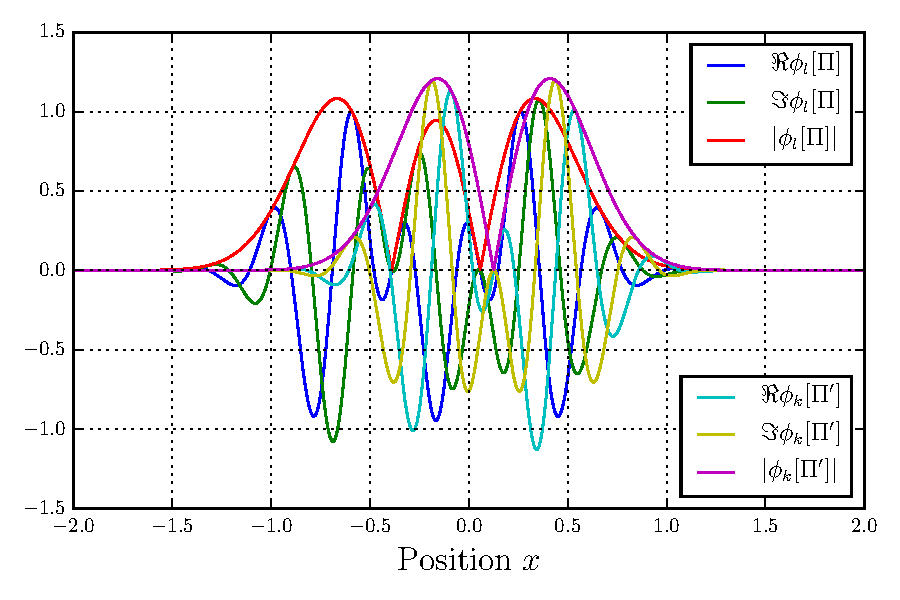
\includegraphics[width=\linewidth]{./fig/overlap_wavepackets.pdf}
    \caption{Wavepackets $\phi_1$ and $\phi_2$.}
    \label{fig:overlap_example_wavepackets}
  \end{subfigure}
  \begin{subfigure}[t]{0.5\linewidth}
    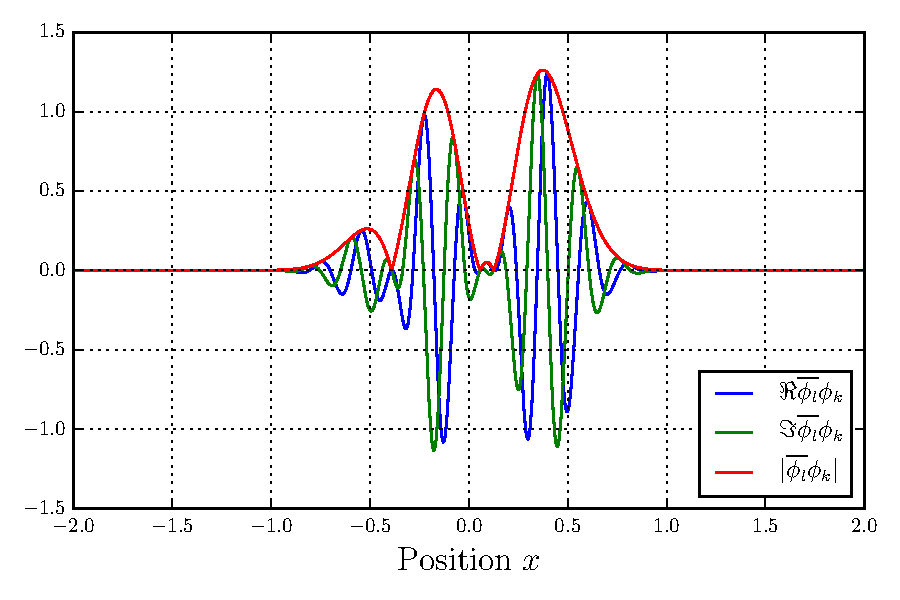
\includegraphics[width=\linewidth]{./fig/overlap_integrand.pdf}
    \caption{Integrand in case of $\phi_1$ and $\phi_2$.}
    \label{fig:overlap_example_integrand}
  \end{subfigure} \\
  \begin{subfigure}[t]{0.5\linewidth}
    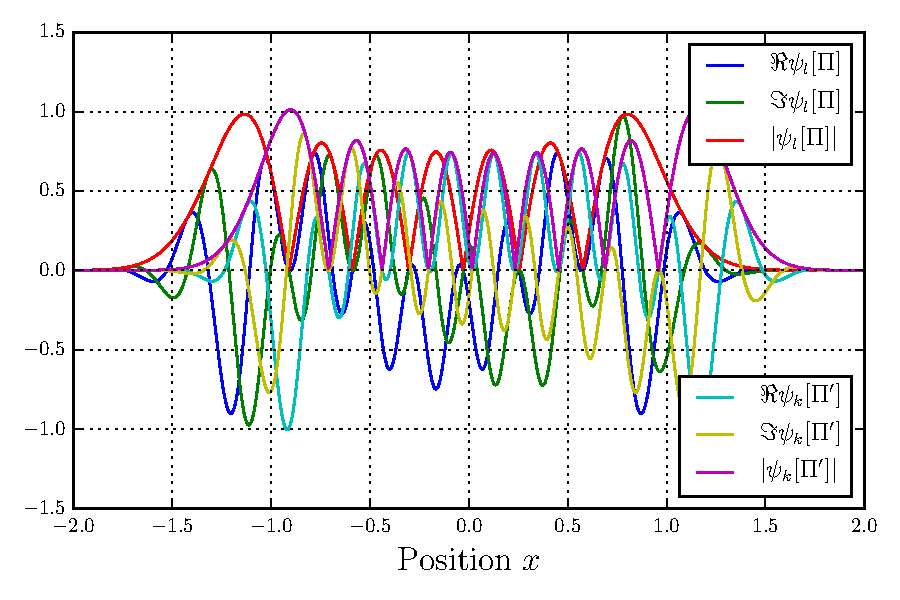
\includegraphics[width=\linewidth]{./fig/overlap_wavepackets_2.pdf}
    \caption{Wavepackets $\phi_8$ and $\phi_6$.}
    \label{fig:overlap_example_wavepackets_2}
  \end{subfigure}
  \begin{subfigure}[t]{0.5\linewidth}
    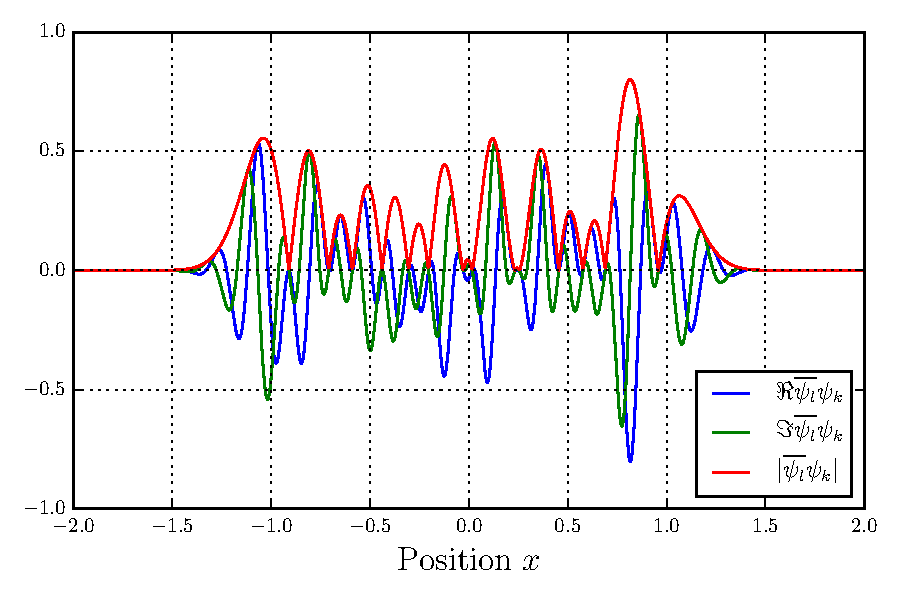
\includegraphics[width=\linewidth]{./fig/overlap_integrand_2.pdf}
    \caption{Integrand in case of $\phi_8$ and $\phi_6$.}
    \label{fig:overlap_example_integrand_2}
  \end{subfigure}
  \caption{\label{fig:overlap_example}
  Examples of wavepackets $\phi_k$ and $\phi_l$ and the integrand $\conj{\phi_k} \phi_l$.
  The parameter sets are
  $q_k = \frac{1}{8}$, $p_k = -\frac{1}{2}$,
  $Q_k = \frac{9}{10}$, $P_k = \frac{10}{9}\imath$
  and
  $q_l = -\frac{1}{6}$, $p_l = \frac{2}{5}$,
  $Q_l = 1$, $P_l = \imath$.
  The scaling parameter is $\varepsilon = \frac{1}{\sqrt{10}} \approx 0.316$.
  Note that the indices $k$ and $l$ typically range up to a few tens
  and this $\varepsilon$ is not very small.}
\end{figure}


\subsection{Combining different oscillators}


Combining the two oscillators is actually a straight-forward computation,
however it is very error prone, big chances are that we miss a transpose
or conjugate somewhere. To simplify the notation we define the matrix:
\begin{equation}
  \mat{\Gamma_i} \assign \mat{P_i}\mat{Q_i}\inv
\end{equation}
and start with computing $\conj{g_k}$:
\begin{equation*}
\begin{split}
 \conj{g_k}
 & =
 \frac{1}{2}\conj{\dotp{\vec{x}-\vec{q_k}}{\mat{\Gamma_k} \left(\vec{x}-\vec{q_k}\right)}}
 +\conj{\dotp{\vec{p_k}}{\vec{x}-\vec{q_k}}} \\
 & =
 \frac{1}{2} \left(
                \conj{\dotp{\vec{x}}{\mat{\Gamma_k} \vec{x}}}
               -\conj{\dotp{\vec{x}}{\mat{\Gamma_k} \vec{q_k}}}
               -\conj{\dotp{\vec{q_k}}{\mat{\Gamma_k} \vec{x}}}
               +\conj{\dotp{\vec{q_k}}{\mat{\Gamma_k} \vec{q_k}}}
              \right)
 + \conj{\dotp{\vec{p_k}}{\vec{x}}}
 - \conj{\dotp{\vec{p_k}}{\vec{q_k}}} \\
 & =
 \frac{1}{2} \left(
               \vec{x}\H \mat{\Gamma_k}\H \vec{x}
              -\vec{q_k}\H \mat{\Gamma_k}\H \vec{x}
              -\vec{x}\H \mat{\Gamma_k}\H \vec{q_k}
              +\vec{q_k}\H \mat{\Gamma_k}\H \vec{q_k}
              \right)
 + \vec{x}\H \vec{p_k} - \vec{q_k}\H \vec{p_k} \,.
\end{split}
\end{equation*}
Next we add $g_l$ and simplify the following expression:
\begin{equation*}
\begin{split}
 -\conj{g_k} + g_l
 = &
 -\frac{1}{2} \left(
               \vec{x}\H \mat{\Gamma_k}\H \vec{x}
              -\vec{q_k}\H \mat{\Gamma_k}\H \vec{x}
              -\vec{x}\H \mat{\Gamma_k}\H \vec{q_k}
              +\vec{q_k}\H \mat{\Gamma_k}\H \vec{q_k}
              \right)
 - \left(\vec{x}\H \vec{p_k} - \vec{q_k}\H \vec{p_k}\right) \\
 & +
  \frac{1}{2} \left(
                \vec{x}\H \mat{\Gamma_l} \vec{x}
               -\vec{x}\H \mat{\Gamma_l} \vec{q_l}
               -\vec{q_l}\H \mat{\Gamma_l} \vec{x}
               +\vec{q_l}\H \mat{\Gamma_l} \vec{q_l}
              \right)
 + \left(\vec{p_l}\H \vec{x} - \vec{p_l}\H \vec{q_l}\right) \\
 = &
 \frac{1}{2} \left(\vec{x}\H \mat{\Gamma_l} \vec{x} - \vec{x}\H \mat{\Gamma_k}\H \vec{x}\right)
 +
 \frac{1}{2} \left(
               \vec{q_k}\H \mat{\Gamma_k}\H \vec{x}
              +\vec{x}\H \mat{\Gamma_k}\H \vec{q_k}
              -\vec{x}\H \mat{\Gamma_l} \vec{q_l}
              -\vec{q_l}\H \mat{\Gamma_l} \vec{x}
             \right) \\
 & +
 \left(\vec{p_l}\H \vec{x} - \vec{x}\H \vec{p_k}\right)
 + \frac{1}{2} \left(
                 \vec{q_l}\H \mat{\Gamma_l} \vec{q_l}
                -\vec{q_k}\H \mat{\Gamma_k}\H \vec{q_k}
               \right)
 + \left(\vec{q_k}\H \vec{p_k} - \vec{p_l}\H \vec{q_l}\right) \\
 = &
 \frac{1}{2} \vec{x}\H \left(\mat{\Gamma_l} - \mat{\Gamma_k}\H\right) \vec{x}
 + \frac{1}{2} \left(
                 \vec{q_k}\H \mat{\Gamma_k}\H \vec{x}
                -\vec{q_l}\H \mat{\Gamma_l} \vec{x}
                +\vec{q_k}\T \conj{\mat{\Gamma_k}} \conj{\vec{x}}
                -\vec{q_l}\T \mat{\Gamma_l}\T \conj{\vec{x}}
               \right) \\
 & +
 \left(\vec{p_l}\H \vec{x} - \vec{p_k}\T \conj{\vec{x}}\right)
 + \frac{1}{2} \left(
                 \vec{q_l}\H \mat{\Gamma_l} \vec{q_l}
                -\vec{q_k}\H \mat{\Gamma_k}\H \vec{q_k}
               \right)
 + \left(\vec{q_k}\H \vec{p_k} - \vec{p_l}\H \vec{q_l}\right) \,.
\end{split}
\end{equation*}
In the end we find a general quadratic oscillator of the common expanded
normal form
% Use $\vec{b}\T \vec{x}$ or rather $\vec{b}\H \vec{x}$?
% $g(\vec{x}) = \vec{x}\H \mat{A} \vec{x} + \vec{b}\H \vec{x} + c$
$g(\vec{x}) = \vec{x}\H \mat{A} \vec{x} + \vec{b}\T \vec{x} + c$
where careful computation gives:
\begin{equation}\label{eq:combined_oscillators}
\begin{split}
  \mat{A} & = \frac{1}{2} \left(\mat{\Gamma_l} - \mat{\Gamma_k}\H \right) \\
%   \vec{b} & = \left(\frac{1}{2} \left(
%                                   \vec{q_k}\H \mat{\Gamma_k}\H
%                                  -\vec{q_l}\H \mat{\Gamma_l}
%                                  +\vec{q_k}\T \conj{\mat{\Gamma_k}}
%                                  -\vec{q_l}\T \mat{\Gamma_l}\T
%                                 \right)
%                 + \left(\vec{p_l}\H - \vec{p_k}\T\right)
%               \right)\H \\
%           & = \frac{1}{2} \left(
%                             \mat{\Gamma_k} \vec{q_k}
%                            -\mat{\Gamma_l}\H \vec{q_l}
%                            +\mat{\Gamma_k}\T \conj{\vec{q_k}}
%                            -\conj{\mat{\Gamma_l}} \conj{\vec{q_l}}
%                           \right)
%               + \left(\vec{p_l} - \conj{\vec{p_k}}\right) \\
  \vec{b} & = \left(\frac{1}{2} \left(
                                  \vec{q_k}\H \mat{\Gamma_k}\H
                                 -\vec{q_l}\H \mat{\Gamma_l}
                                 +\vec{q_k}\T \conj{\mat{\Gamma_k}}
                                 -\vec{q_l}\T \mat{\Gamma_l}\T
                                \right)
                + \left(\vec{p_l}\H - \vec{p_k}\T\right)
              \right)\T \\
          & = \frac{1}{2} \left(
                            \conj{\mat{\Gamma_k}} \conj{\vec{q_k}}
                           -\mat{\Gamma_l}\T \conj{\vec{q_l}}
                           +\mat{\Gamma_k}\H \vec{q_k}
                           -\mat{\Gamma_l} \vec{q_l}
                          \right)
              + \left(\conj{\vec{p_l}} - \vec{p_k}\right) \\
  c & = \frac{1}{2} \left(
                      \vec{q_l}\H \mat{\Gamma_l} \vec{q_l}
                     -\vec{q_k}\H \mat{\Gamma_k}\H \vec{q_k}
                    \right)
        + \left(\vec{q_k}\H \vec{p_k} - \vec{p_l}\H \vec{q_l}\right)
\end{split}
\end{equation}
and we assumed that $\vec{x}$ is real. Be sure to pay attention to
the fact that here we have $\vec{b}\T$ only instead of $\vec{b}\H$.
The matrix $\mat{A}$ has a special property, both its real and
imaginary parts are symmetric while the matrix itself is in general
\emph{not} Hermitian. This places the matrix right outside the convenient
set of normal matrices, which implies that it is not diagonalizable
by unitary matrices,  an important  consequence as we will see later.


\section{Numerical steepest descent}

\subsection{Overview and summary of the ideas}


A typical example of a highly oscillatory integral looks like:
\begin{equation}
  I = \int_{\Omega} f(\vec{x}) \, \exp(\imath \omega g(\vec{x})) \di{\vec{x}}
\end{equation}
where the non-oscillatory function $g:\mathbb{R}^N \rightarrow \mathbb{C}$
is called the oscillator and the also non-oscillatory function
$f:\mathbb{R}^N \rightarrow \mathbb{C}$ the envelope. The parameter
$\omega \in \mathbb{R}^{+}$ is the frequency. Often one looks at the
asymptotic behavior for $\omega \rightarrow \infty$. In our setting
this parameter $\omega$ has a fixed and finite value.
Finally there is the domain of integration denoted by $\Omega \subset \mathbb{R}^N$.
In the theory shown so far this is a bounded subset of $\mathbb{R}^N$.
Figure~\ref{fig:oscillatory_example_2d} shows a particular
example of such a nasty integrand.

\begin{figure}[h]
  \centering
  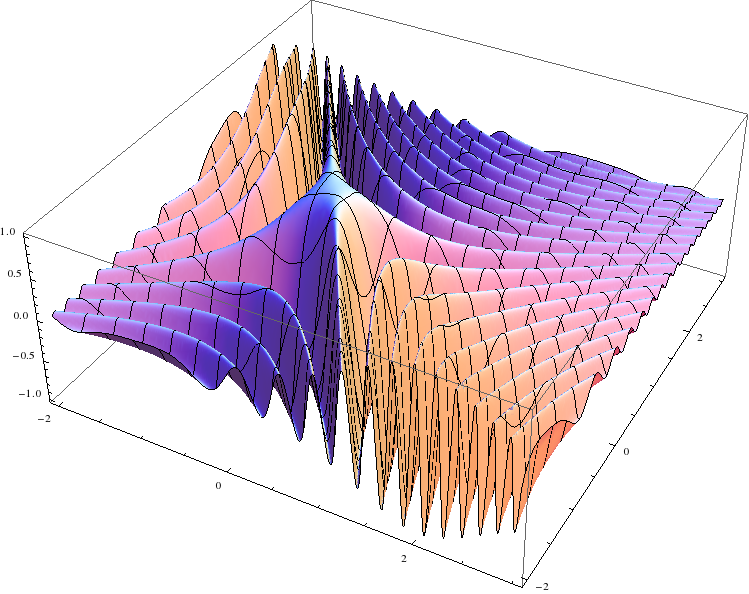
\includegraphics[width=0.6\linewidth]{fig/oscillatory_example_2d.png}
  \caption{Oscillatory integrand of the integral
  $\int_{-2}^3 \int_{-2}^3 \frac{e^{5 \imath (x^2-x y-y^2)}}{1 + {(x+y)}^2} \di{x} \di{y}  $
  with envelope $f(x,y) = \frac{1}{1 + {(x+y)}^2}$ and a quadratic oscillator
  $g(x,y) = x^2 - x y - y^2$ at low frequency of $\omega = 5$.}
  \label{fig:oscillatory_example_2d}
\end{figure}

For our problem at hand, computing overlap integrals, we will need to integrate
over the whole space in $N$ dimensions and hence set $\Omega = \mathbb{R}^N$ in
\eqref{eq:hoi}.
There are two essential observations to be made about the
oscillatory part $\exp\left(\imath \omega g\left(\vec{x}\right) \right)$
of any such integral. First, this expression does decay exponentially
fast for increasing $\Im g(z)$ and second, it does not oscillate for
constant $\Re g(z)$. This can easily be seen by expanding complex numbers:
\begin{equation*}
  e^{\imath \omega g(z)}
  =
  e^{\imath \omega (\Re g(z) + \imath \Im g(z))}
  =
  e^{\imath \omega \Re g(z)}
  e^{- \omega \Im g(z)} \,.
\end{equation*}
The main idea behind the \emph{numerical steepest descent} method is therefore
to transform the integrand such that it is no longer oscillatory but
rather exponentially decaying. For this we need to find a coordinate
transformation $z = h(\tau)$ such that the \emph{real} part of $g(z)$
is constant. In a second step we then apply Cauchy's Theorem for contour
integrals along the path $h(\tau)$.

Let us look again at the plot in Figure~\ref{fig:oscillatory_example_2d}
and ask the question in which regions of $\Omega$ the integrand contributes most
to the value of the integral. By intuition one would say, at least asymptotically
for $\omega \rightarrow \infty$, that oscillations in the integrand generally approximately
cancel out and mainly places with locally no oscillations contribute to the value.
Regions showing no oscillations are \emph{stationary points} where
$\nabla g(\vec{x}) = \vec{0}$ on one hand and so called \emph{resonance points}
defined by the condition $\nabla g(\vec{x}) \perp \partial \Omega$ on the other.
In the one-dimensional case one can forget about the complications around resonance
points and just take care of the endpoints of the interval $[a, b] = \Omega$. In our
case there is no surface $\partial \Omega$ anyway as we compute over the whole space
$\mathbb{R}^N$.

In the following we briefly consider the one-dimensional integral over the interval
$[a,b]$ and walk through the major steps involved in the procedure. We can find all
stationary points ${\{x_{j}^{*}\}}_{j}$ from equating the gradient to zero (assuming
the equation is indeed solvable):
\begin{equation}
  \nabla_{x} \, g(x) = 0 \,.
\end{equation}
The set of contributing points is then:
\begin{equation}
  \Theta := \{a, b\} \cup {\{x^{*}_j\}}_j \,.
\end{equation}
Next, we set up the so called \emph{path equation} to compute the coordinate
transformation $h(\tau)$ or equivalently the path of integration. This has to
be done locally at all contributing points. Hence, for all $\xi \in \Theta$:
\begin{equation}
  g(h_\xi(\tau)) = g(\xi) + \imath \tau \,.
\end{equation}
Solving these equations yields a bunch of paths $h_{\xi}(\tau)$. Each one is
indexed by the point $\xi$ it starts at\footnote{Note that this is not the full truth.
In case of multi-valued inverses of $g$ at the point $\xi$ it can happen that
$h_\xi(0) \neq \xi$. With $g (x)= x^2$ and $\xi = 3$ we find $h_3(\tau) = \pm \sqrt{9+\imath\tau}$
and $h_3(0) = \pm 3 \neq 3$.}
and parametrised by $\tau \in \mathbb{R}_0^{+}$.
Refer to Figure~\ref{fig:nsd_path_example} for a simple example having only a single
stationary point.

\begin{figure}
  \centering
  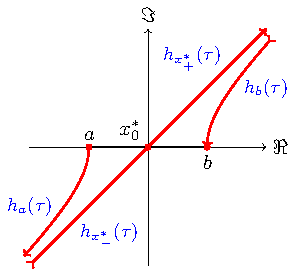
\includegraphics[width=0.6\linewidth]{./fig/nsd_path_figure.pdf}
  \caption{Example of an integral treated by the numerical steepest descent method.
  The oscillator is $g(x) = x^2$ and hence $\partial_x g(x) = 0$ at $x^{*} = 0$.
  Shown are the contributing points $a$, $b$ and $x_0^{*}$ and the paths
  $h_a(\tau)$, $h_b(\tau)$ and $h_{x_0^{*},\pm}(\tau)$ attached to them.
  Instead of integrating directly from $a$ to $b$ along the real axis, we follow
  the red path through the complex plane.}
  \label{fig:nsd_path_example}
\end{figure}

In general, solving the path equation amounts to finding an inverse of $g$. In some cases
this inverse is multi-valued and the path not unique. At the endpoints we can
choose the correct path $h_a(\tau)$ by requiring $h_a(0) = a$ which forces the
path chosen to be really attached to the point $a$. At the stationary points we have
to choose two paths, $h_{x^{*}_j,+}$ and $h_{x^{*}_j,-}$, one of which is considered
incoming and the other outgoing (note that this is not reflected by the parametrisation
in $\tau$), such that the integration contour passes through each stationary point once.
Then we have to make sure that the outgoing path of one stationary point
and the incoming of the next one will lead to the same \emph{valley}. This guarantees
that we can concatenate all paths in the end and obtain a closed contour for integration.
We will not bother too much with these details as they are not relevant for our problem.
Many more details can be found in the original papers~\cite{HV_hoq} and~\cite{HV_cub} by
Huybrechs and Vandewalle. If the path equation can not be solved analytically, not
all is lost as it is possible to work with numerical path approximations, see~\cite{AH_nsd_pa}.
By the formal structure of the semiclassical wavepackets, the path equation in our case is always
a multivariate quadratic form which we can solve explicitly.

Now it is time to assemble the parts. For each path attached at a point $\xi \in \Theta$
we perform the transformation $x \mapsto h_{\xi}(\tau)$. Doing this change of variable
will give a bunch of new integrals, one or two for each $\xi$:
\begin{equation}\label{eq:single_path_integral}
\begin{split}
  J[\xi] & := e^{\imath \omega g(\xi)}
              \int_{0}^{\infty}
                f(h_{\xi}(\tau)) \,
                h_{\xi}^{\prime}(\tau) \,
                e^{-\omega \tau} \,
              \mathrm{d}\tau \\
         & = \frac{e^{\imath \omega g(\xi)}}{\omega}
              \int_{0}^{\infty}
                f\left(h_{\xi}\left(\frac{\tau}{\omega}\right)\right) \,
                h_{\xi}^{\prime}\left(\frac{\tau}{\omega}\right) \,
                e^{-\tau} \,
              \mathrm{d}\tau \,.
\end{split}
\end{equation}
We continue by applying Cauchy's theorem:
\begin{equation}\label{eq:cauchy}
      I = e^{\imath \omega g(a)} J[a]
        + \sum_{j} \left(J[x_{j,+}^{*}] - J[x_{j,-}^{*}]\right)
        - e^{\imath \omega g(b)} J[b]
\end{equation}
which is valid for the correct choice of paths. We glue together all the paths
to a single long path connecting the endpoints $a$ and $b$ while wandering around
in the complex plane and visiting each stationary point once. Obviously we have to
be very careful, avoid crossing branch cuts and be aware of all potential poles.
In our case there is no danger around because $f$ is simply a polynomial.

Up to now we just transformed the problem, nothing more. The new task is to
compute by quadrature all the integrals~\eqref{eq:single_path_integral} and
there can be exponentially many of these in higher dimensions. For this type of
semi-finite integrals Gauss-Laguerre quadrature with nodes ${\{\gamma_k\}}_{k}$
and weights ${\{w_k\}}_{k}$ seems to be most appropriate:
\begin{equation}
  J[\xi] \approx \frac{e^{\imath \omega g(\xi)}}{\omega}
                 \sum_{k}
                   f\left(h_{\xi}\left(\frac{\gamma_k}{\omega}\right)\right)
                   h_{\xi}^{\prime}\left(\frac{\gamma_k}{\omega}\right)
                   w_k \,.
\end{equation}
Depending on the oscillator and in turn the path $h_{\xi}$ these integrals can be
weakly singular (to be precise, having roots in the denominator) which can in turn
be accounted for by the generalized Gauss-Laguerre quadrature. These singularities
originate from roots involved in the multi-valued inverses of $g$ at some stationary
points.

For our problem we will find that we can always glue together the two opposite
straight line paths at the single stationary point, apply one further transformation and
finally use Gauss-Hermite quadrature. The whole process for computing~\eqref{eq:hoi}
then looks like shown in Figure~\ref{fig:transformation_chain_2}. Performing these
transformations on the first two example wavepackets $\phi_k$ and $\phi_l$ from
Figure~\ref{fig:overlap_example} we can make the plot shown in~\ref{fig:hawp_trafo_example}.

\begin{figure}
  \centering
  \includegraphics[width=\linewidth]{./fig/diagram2.pdf}
  \caption{Steepest descent transformation and integral computation.}
  \label{fig:transformation_chain_2}
\end{figure}

\begin{figure}[h!]
  \centering
  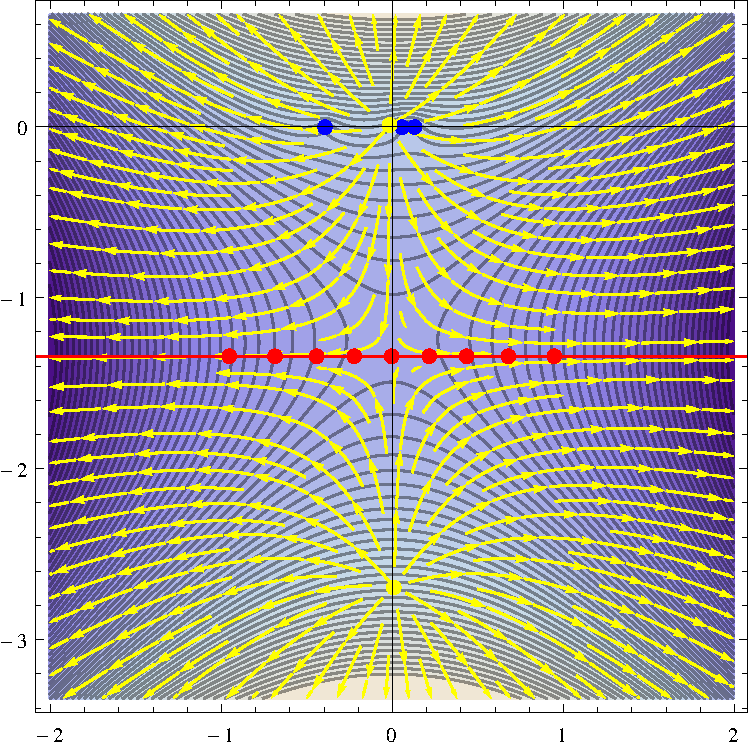
\includegraphics[width=0.8\textwidth]{./fig/stationary_point_example.pdf}
  \caption{Contour levels and zeros (blue) of $|\conj{\phi_{\vec{l}}} \phi_{\vec{k}}|$,
  Gradient field and zeros of $|g|$ (yellow), Path of steepest descent with 9 Gauss Hermite
  quadrature nodes (red), in complex plane.}
  \label{fig:hawp_trafo_example}
\end{figure}


\subsection{Extensions and new concepts}


In the last part we have walked through the very basic concepts of the numerical steepest
descent method. Under some broad assumptions this was proven to work for finite intervals
and an arbitrary number of real stationary points~\cite{HV_hoq}. The extension into higher
dimensions has been worked out~\cite{HV_cub}.
However, the state of the theory is too narrow for our setting. First we need to consider
complex stationary points too. If such a point is near to the real line, it will influence
the oscillator enough to become relevant. Figure~\ref{fig:oscillatory_integral_complex_sp}
for example shows the integrand of:
\begin{equation}\label{eq:nsd_csp_integral_example}
  \int_{-2}^{2} \left(2+x^2\right) e^{50 \imath \left(\delta x + \frac{x^3}{3}\right)} \di{x}
\end{equation}
for different values of the parameter $\delta$. One stationary point is located on the imaginary axis
at $x^{*} = \imath \sqrt{\delta}$ and comes close to the real line. The influence is clearly present
for small values of $\delta$ and soon becomes negligible for larger values.
The general advise for complex stationary points is that the contour should pass through
this point as shown in Figure~\ref{fig:oscillatory_integral_complex_sp_paths},
see section 4.3 in~\cite{HV_hoq}. This will then give an exact
decomposition in the sense of~\eqref{eq:cauchy}. It turns out this works very well for our setting.
Actually, the \emph{only} thing we have is a single stationary point.

\begin{figure}
  \centering
  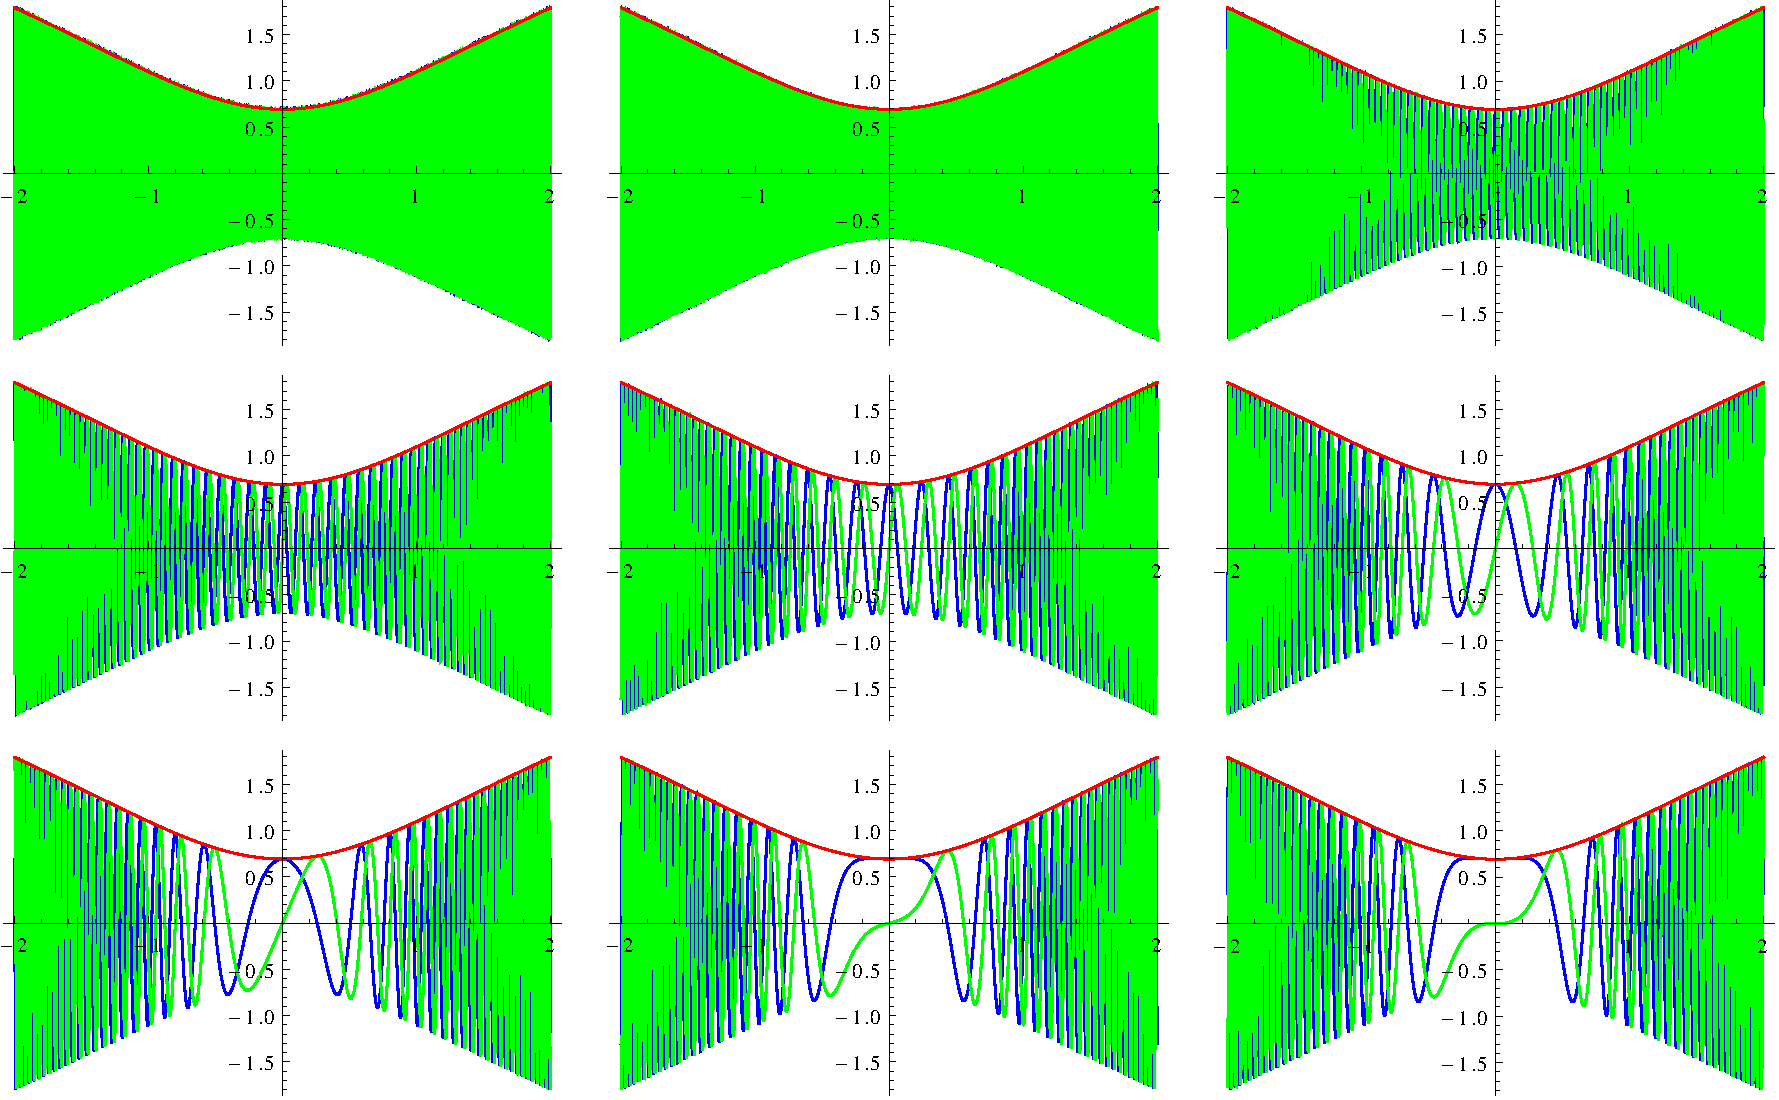
\includegraphics[width=\linewidth]{./fig/oscillatory_integral_complex_sp.pdf}
  \caption{Oscillatory integral on $[-2,2]$ with a stationary point $x^{*}$ at $\imath \sqrt{\delta}$
  shown for several different decreasing values of
  $\delta \in \{10, 5, 2, 1, \frac{1}{2}, \frac{1}{5}, \frac{1}{10}, \frac{1}{100}, 0\}$.}
  \label{fig:oscillatory_integral_complex_sp}
\end{figure}

\begin{figure}
  \centering
  \includegraphics[width=0.8\linewidth]{./fig/nsd_path_csp_figure.pdf}
  \caption{Paths of the integral~\eqref{eq:nsd_csp_integral_example}.
  The two additional paths $h_{x^{*},{\pm}}(\tau)$ go through the complex
  stationary point $x_0^{*}$. The contribution stemming from these two paths
  varies with $\delta$. For $\delta = 1$ it is $\bigO{10^{-16}}$ and the whole
  integral has a value of $I = 0.0317496$ while for $\delta = \frac{1}{5}$ it is
  $0.033533$ which is not negligible given that now $I = 0.0253591$.}
  \label{fig:oscillatory_integral_complex_sp_paths}
\end{figure}

Another direction to extend the theory are infinite regions $\Omega$. In our case we will
need $\Omega = \mathbb{R}^N$. Before we take this step, we look at semi-finite intervals.
For semi-finite intervals $[a, \infty [$ we attach only one single path $h_a(\tau)$ an the
finite endpoint $a$. Details are described by Majidian and can be found in~\cite{H_nsd_sii}. If there
are stationary points, they can be split off into sub-problems over finite intervals.
As an example, we look at the following integral:
\begin{equation}
  I = \int_0^\infty \frac{100}{100 + x^2} \exp\left(\imath \omega e^{\sqrt{x}}\right) \di{x}
\end{equation}
where we set $\omega = 2$. The path is given by the expression:
\begin{equation}
  h_a(\tau) = {\log(1 + \imath\tau)}^2 \,.
\end{equation}
After the change of variables the integral takes the following ugly form:
\begin{equation}
  I = 200 \, e^{\imath \omega}
      \int_0^{\infty}
        \frac{\imath \log(1+\imath\tau) e^{-\omega\tau}}
             {(1 + \imath\tau)\left(100+\log^4(1+\imath\tau)\right)}
      \di{\tau} \,.
\end{equation}

\begin{figure}[h!]
  \begin{subfigure}[t]{0.5\linewidth}
    \centering
    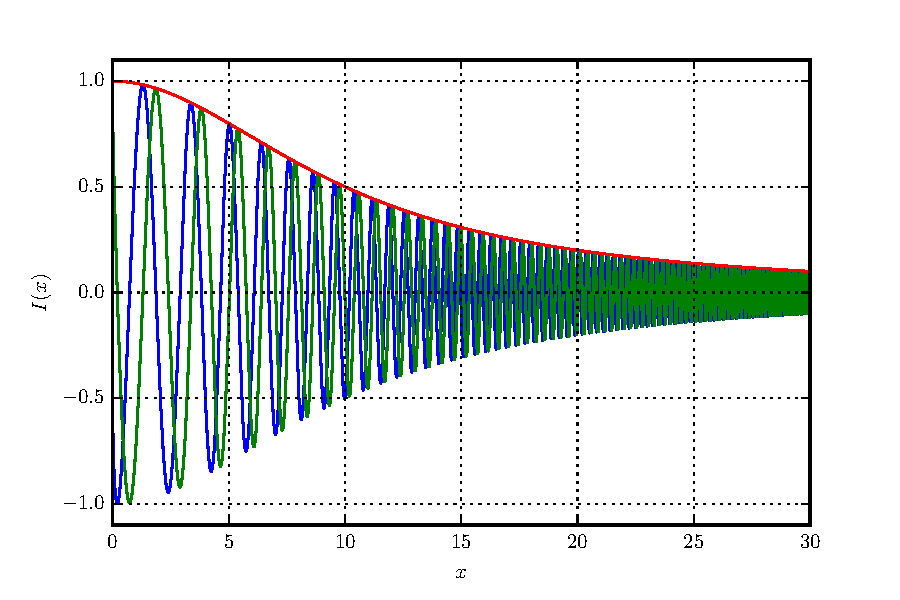
\includegraphics[width=\linewidth]{./fig/oscillatory_example_semiopen.pdf}
    \caption{Oscillatory integrand on $[a, \infty[$.}
    \label{fig:oscillatory_example_semiopen_integrand}
  \end{subfigure}
  \begin{subfigure}[t]{0.5\linewidth}
    \centering
    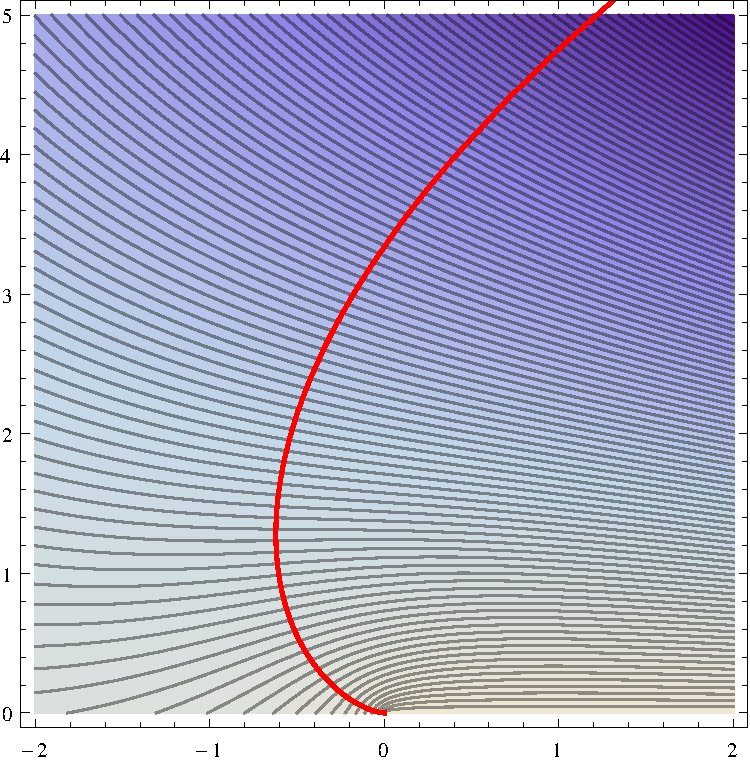
\includegraphics[height=4cm]{./fig/oscillatory_example_semiopen_path.pdf}
    \caption{Path of steepest descend.}
    \label{fig:oscillatory_example_semiopen_path}
  \end{subfigure}
  \caption{\label{fig:oscillatory_example_semiopen}
  Example of an oscillatory integrand on a semi-finite interval and the
  corresponding path of steepest descend.}
\end{figure}

Given all these parts, the extension to infinite intervals becomes simple.
We just split the overall interval $]-\infty, \infty[$ into a union of three
intervals: $]-\infty, a]$, $[a,b]$ and $[b,\infty[$. The reason to choose three
instead of only two semi-finite intervals is the stationary point which we know
to exist in our specific case. With this splitting we can put it into the finite
interval and know that it gets handled correctly. Of course the paths at the points
$a$ and $b$ will be traversed two times in reversed directions and hence cancel out.
The only thing that remains is the pair of paths attached to the single complex stationary
point $x^{*}$. This works the same in any number of dimensions where we resolve the nested
integrals one after the other. By gluing together the two paths of opposite direction
we end up with a cross of exactly $N$ straight paths. Therefore the number and nesting
depth of integrals to perform does \emph{not} grow compared to direct integration.
This is of course very fortunate.


\section{A first exemplary computation}
\label{sec:mv_triag_plain}


In this section we show a complete computation for a three
dimensional example. The purpose is to give the reader a
rough feeling on how the overall process for our specific
overlap integral works. We will write down all the technical
details in the next section.

For the following computation we assume that
the upper triangular matrix $\mat{T}$ is given:
\begin{equation}
 \mat{T} =
 \begin{pmatrix}
  t_{1,1} & t_{1,2} & t_{1,3} \\
  0       & t_{2,2} & t_{2,3} \\
  0       & 0       & t_{3,3}
 \end{pmatrix}
\end{equation}
and we study the oscillator $g$ given by:
\begin{equation}
 g\left(\vec{x}\right) := \vec{x}\H \mat{T} \vec{x} \,,
\end{equation}
i.e.:
\begin{equation}
 g\left(x_1, x_2, x_3\right) = t_{1,1} x_1^2 + t_{2,2} x_2^2 + t_{3,3} x_3^2
                             + t_{1,2} x_1 x_2 + t_{1,3} x_1 x_3 + t_{2,3} x_2 x_3 \,.
\end{equation}
The integral we want to compute is:
\begin{equation}\label{eq:mv_original_integral}
  I = \iiint_{-\infty}^{\infty} f\left(\vec{x}\right) \exp\left(\imath \omega g\left(\vec{x}\right) \right) \mathrm{d}\vec{x}
    = \iiint_{-\infty}^{\infty} i\left(x_1, x_2, x_3\right) \mathrm{d}x_1 \mathrm{d}x_2 \mathrm{d}x_3
\end{equation}
where we collapsed the internals into a single function $i\left(x_1, x_2, x_3\right)$
for reasons of notation. By using the expanded form of $g$ the integral can be written as:
\begin{equation}
\begin{alignedat}{2}
 I & = \iiint f\left(\vec{x}\right)
             & & \exp\left(\imath \omega \left(t_{1,1} x_1^2 + t_{1,2} x_1 x_2 + t_{1,3} x_1 x_3\right) \right) \\
             & & & \exp\left(\imath \omega \left(t_{2,2} x_2^2 + t_{2,3} x_2 x_3\right) \right) \\
             & & & \exp\left(\imath \omega \left(t_{3,3} x_3^2 \right) \right)
       \mathrm{d}\vec{x} \\
   & = \iiint f\left(\vec{x}\right)
             & & \exp\left(\imath \omega \left(t_{1,1} x_1^2 + t_{1,2} x_1 x_2 + t_{1,3} x_1 x_3\right) \right)
            \mathrm{d}x_1 \\
             & & & \exp\left(\imath \omega \left(t_{2,2} x_2^2 + t_{2,3} x_2 x_3\right) \right)
            \mathrm{d}x_2 \\
             & & & \exp\left(\imath \omega \left(t_{3,3} x_3^2 \right) \right)
            \mathrm{d}x_3 \,.
\end{alignedat}
\end{equation}
We pulled out of each integral the parts of the oscillator
independent of the integration variable. Therefore we split
the full oscillator $g$ additively into $N$ parts $g_i$:
\begin{equation}
  g(\vec{x}) = g_1(x_1, x_2, x_3) + g_2(x_2, x_3) + g_3(x_3)\,.
\end{equation}
Beginning with the inner most one, we can resolve these onion-like
nested integrals one by one. From:
\begin{equation}
 \int_{-\infty}^{\infty} f\left(\vec{x}\right)
   \exp\left(\imath \omega \left(t_{1,1} x_1^2 + t_{1,2} x_1 x_2 + t_{1,3} x_1 x_3\right) \right)
 \mathrm{d}x_1
\end{equation}
we find the relevant oscillator $g_1(x_1, x_2, x_3)$ to be:
\begin{equation}
  g_1\left(x_1\right) \assign t_{1,1} x_1^2 + t_{1,2} x_1 x_2 + t_{1,3} x_1 x_3 \,.
\end{equation}
where we treat the variables $x_2$ and $x_3$ as parameters.
Let $x_1^*$ denote the (perhaps complex) stationary point\footnote{A
\emph{stationary point} $\vec{x}^{*}$ is the solution to the equation
$\nabla g(\vec{x}) = 0$, a point where the derivative of the oscillator vanishes.
Actually, $x_i^{*}$ is not a \emph{point}.
It depends on $x_{i+1}$ up to $x_N$, so $x_i^{*}$ is rather a $N-i$
dimensional object.} of $g_1$. The path equation then is:
\begin{equation}
  g_1\left(h_1(\tau_1)\right) = g_1\left(x_1^{*}\right) + \imath \tau_1
\end{equation}
which, expanded out, is:
\begin{gather}
  t_{1,1} h_1^2 + t_{1,2} h_1 x_2 + t_{1,3} h_1 x_3 = k_1(x_2, x_3) + \imath \tau_1 \\
  t_{1,1} h_1^2 + t_{1,2} h_1 x_2 + t_{1,3} h_1 x_3 - k_1(x_2, x_3) - \imath \tau_1 = 0 \,.
\end{gather}

Since the expression $g_1\left(x_1^{*}\right)$ depends parametrically on
$x_2$ and $x_3$, we denote the whole thing by $k_1\left(x_2, x_3\right)$.
As $k_1$ does not depend on $x_1$ we can pull it out from the
current integral. We will see later how to deal explicitly with
all the $k_i$ depending on all the variables $\left(x_{i+1}, \ldots ,x_N\right)$.

By solving the last equation we obtain the complex integration path
$h_1\left(\tau_1\right)$ parametrised in the variable $\tau_1 \in [0,\infty[$.
Note that, at this point $h_1$ still depends on $x_2$ and $x_3$.
Transforming the integrand of this first integral we find:
\begin{equation*}
 i_1\left(\tau_1, x_2, x_3\right) := f\left(h_1(\tau_1, x_2, x_3), x_2, x_3\right)
                                     \exp\left(\imath \omega k_1\left(x_2, x_3\right) \right)
                                     \exp\left(- \omega \tau_1 \right)
                                     \pdiff{h_1\left(\tau_1, x_2, x_3\right)}{\tau_1}
\end{equation*}
and for the integral itself:
\begin{equation*}
\begin{split}
  I_1\left(x_2, x_3\right) & = \int_0^{\infty} i_1\left(\tau_1, x_2, x_3\right) \mathrm{d}\tau_1 \\
                           & = \exp\left(\imath \omega \,k_1\!\left(x_2, x_3\right) \right)
                               \int_0^{\infty} f\left(h_1(\tau_1, x_2, x_3), x_2, x_3\right)
                                               \exp\left(- \omega \tau_1 \right)
                                               \pdiff{h_1\left(\tau_1, x_2, x_3\right)}{\tau_1}
                               \mathrm{d}\tau_1 \,.
\end{split}
\end{equation*}
We pull out the prefactor $\exp\left(\imath \omega \,k_1\!\left(x_2, x_3\right) \right)$
constant with respect to $x_1$ and call it $p_1\left(x_2, x_3\right)$.
Then we continue with the second integral where we have to merge parts of
$p_1$ into $g_2$ (we will show the details later):
\begin{equation}
  \int_{-\infty}^{\infty} I_1\left(x_2, x_3\right)
                          \exp\left(\imath \omega \,k_1\!\left(x_2, x_3\right) \right)
                          \exp\left(\imath \omega \left(t_{2,2} x_2^2 + t_{2,3} x_2 x_3\right) \right)
  \mathrm{d}x_2 \,.
\end{equation}
The oscillator is given now by:
\begin{equation}
 g_2(x_2) = t_{2,2} x_2^2 + t_{2,3} x_2 x_3 + k_1(x_2, x_3)
\end{equation}
and depends parametrically on $x_3$. For the path we have:
\begin{equation}
  g_2\left(h_2(\tau_2)\right) = g_2\left(x_2^{*}\right) + \imath \tau_2
\end{equation}
which in turn can be resolved to:
\begin{equation}
  t_{2,2} h_2^2 + t_{2,3} h_2 x_3 + k_1(h_2, x_3) = k_2(x_3) + \imath \tau_2
\end{equation}
and then:
\begin{equation}
  t_{2,2} h_2^2 + t_{2,3} h_2 x_3 + k_1(h_2, x_3) - k_2(x_3) - \imath \tau_2 = 0 \,.
\end{equation}
Using this path $h_2$ obtained from solving the quadratic
path equation we get the new integrand as:
\begin{equation}
  i_2\left(\tau_2, x_3\right) := I_1\left(h_2(\tau_2, x_3), x_3\right)
                                 \exp\left(\imath \omega \,k_2\!\left(x_3\right) \right)
                                 \exp\left(- \omega \tau_2 \right)
                                 \pdiff{h_2\left(\tau_2, x_3\right)}{\tau_2} \,.
\end{equation}
And then in turn we write for the integral:
\begin{equation*}
\begin{split}
  I_2\left(x_3\right) & = \int_0^{\infty} i_2\left(\tau_2, x_3\right) \mathrm{d}\tau_2 \\
                      & = \exp\left(\imath \omega \,k_2\!\left(x_3\right) \right)
                          \int_0^{\infty} I_1\left(h_2(\tau_2, x_3), x_3\right)
                                          \exp\left(- \omega \tau_2 \right)
                                          \pdiff{h_2\left(\tau_2, x_3\right)}{\tau_2}
                          \mathrm{d}\tau_2 \,.
\end{split}
\end{equation*}
where we pull out $p_2 \assign \exp\left(\imath \omega k_2\left(x_3\right) \right)$.
For the third and outer-most integral we can write:
\begin{equation}
  \int_{-\infty}^{\infty} I_2\left(x_3\right)
                          \exp\left(\imath \omega k_2\left(x_3\right) \right)
                          \exp\left(\imath \omega t_{3,3} x_3^2\right)
  \mathrm{d}x_3 \,.
\end{equation}
Once more, we first extract the oscillator expression:
\begin{equation}
  g_3\left(x_3\right) = t_{3,3} x_3^2 + k_2(x_3)\,.
\end{equation}
The corresponding path equation is:
\begin{equation}
\begin{split}
  g_3\left(h_3\left(\tau_3\right)\right) & = g_3(x_3^{*}) + \imath \tau_3 \\
  t_{3,3} h_3^2 + k_2(h_3) & = k_3 + \imath \tau_3 \\
  t_{3,3} h_3^2 + k_2(h_3) - k_3 - \imath \tau_3 & = 0 \,.
\end{split}
\end{equation}
Note that the variable $k_3$ does not depend on any $x_i$ anymore.
With the solution $h_3$ our integrand reads:
\begin{equation}
 i_3\left(\tau_3\right) := I_2\left(h_3(\tau_3)\right) \exp\left(\imath \omega k_3 \right)
                           \exp\left(- \omega \tau_3 \right) \pdiff{h_3\left(\tau_3\right)}{\tau_3}
\end{equation}
and the integral becomes:
\begin{equation}
\begin{split}
  I_3 & = \int_0^{\infty} i_3\left(\tau_3\right) \mathrm{d}\tau_3 \\
      & = \exp\left(\imath \omega k_3\right)
          \int_0^{\infty} I_2\left(h_3(\tau_3)\right)
                          \exp\left(- \omega \tau_3 \right)
                          \pdiff{h_3\left(\tau_3\right)}{\tau_3}
          \mathrm{d}\tau_3 \,.
\end{split}
\end{equation}

Finally we obtain the solution of the original integral:
\begin{equation*}
\begin{split}
  I & = I_3 = \int_0^{\infty} I_2\left(h_3(\tau_3)\right) \ldots \mathrm{d}\tau_3 \\
    & = \int_0^{\infty}
          \int_0^{\infty} I_1\left(h_2(\tau_2, h_3(\tau_3)), h_3(\tau_3)\right)
          \ldots \mathrm{d}\tau_2
        \ldots \mathrm{d}\tau_3 \\
    & = \int_0^{\infty}
          \int_0^{\infty}
            \int_0^{\infty} f\left(h_1(\tau_1, h_2(\tau_2, h_3(\tau_3)), h_3(\tau_3)),
                                   h_2(\tau_2, h_3(\tau_3)),
                                   h_3(\tau_3)
                             \right)
            \ldots \mathrm{d}\tau_1
          \ldots \mathrm{d}\tau_2
        \ldots \mathrm{d}\tau_3 \\
    & = \int_0^{\infty}
          \int_0^{\infty}
            \int_0^{\infty} f\left(\tilde{h}_1(\tau_1, \tau_2, \tau_3),
                                   \tilde{h}_2(\tau_2, \tau_3),
                                   \tilde{h}_3(\tau_3)
                             \right)
            \ldots \mathrm{d}\tau_1
          \ldots \mathrm{d}\tau_2
        \ldots \mathrm{d}\tau_3 \\
\end{split}
\end{equation*}
This is the nasty return of the recursive scheme here.
The final denested paths $\tilde{h}_1\left(\tau_1, \tau_2, \tau_3\right)$ and
$\tilde{h}_2\left(\tau_2, \tau_3\right)$ can be found from
$h_1\left(\tau_1, x_2, x_3\right)$ and $h_2\left(\tau_2, x_3\right)$
by substituting $h_2$ for $x_2$ and $h_3$ for $x_3$.


\section{Systematic approach}


In this section we look at the general $N$ dimensional case
and follow a very systematic approach. We will investigate
all the technical details omitted during the example from
the last section.


\subsection{General triangular oscillators}


Given a general, probably complex, upper triangular
matrix $\mat{T}$ of dimension $N \times N$ we look at
the oscillator given by:
\begin{equation}\label{eq:triangular_oscillator}
  g\left(\vec{x}\right) = \vec{x}\H \mat{T} \vec{x} \,.
\end{equation}
The process of pulling out from each integral parts that do not
depend on the respective variable of integration yields the
additive decomposition of $g$:
\begin{equation}
  g\left(\vec{x}\right) = g\left(x_1, \ldots, x_N\right) = \sum_{i=1}^N g_i(x_i, \ldots, x_N) \,.
\end{equation}
At each shell $i$ of the onion we exclusively work with the
partial oscillator $g_i$. In general the coefficients of this
oscillator are given by the $i$-th row of $\mat{T}$:
\begin{equation}\label{eq:general_partial_gi}
\boxed{
  g_i\left(x_i, x_{i+1}, \ldots, x_N\right)
  \assign t_{i,i} x_i^2 + \sum_{j=i+1}^{N} t_{i,j} x_i x_j \,.
}
\end{equation}


\subsection{Computing stationary points}


As we know from the theory of numerical steepest descent, we need
to find the stationary points of an oscillator $g_i$. It is possible
to do this by a straight forward computation.

First we take the partial derivative of $g_i$, in fact we have:
\begin{equation}
 \dot{g}_i \assign \pdiff{g_i}{x_i}
              = 2 t_{i,i} x_i + \sum_{j=i+1}^{N} t_{i,j} x_j
\end{equation}
The location of the stationary point is implicitly specified by:
\begin{equation}
  \dot{g}_i = 0 \,.
\end{equation}
Solving this equation for the stationary point $x^*_i$ explicitly we get:
\begin{equation}\label{eq:stationary_point_xi}
\boxed{
  x_i^*
  \assign x_i^{*}\left(x_{i+1}, \ldots, x_N\right)
  = - \frac{\sum_{j=i+1}^{N} t_{i,j} x_j}{2 t_{i,i}} \,.
}
\end{equation}
It is important to remember that at level $i$ the point $x_i^*$
is stationary with respect to the coordinate $x_i$ but
depends on the variables $x_{i+1}$ through $x_N$.

Plugging this solution $x_i^*$ into $g_i$ from~\eqref{eq:general_partial_gi}
we can compute the expressions $k_i$ explicitly:
\begin{equation*}
\begin{split}
  g_i(x_i^*, x_{i+1}, \ldots, x_N)
  & =
  t_{i,i} {\left(
    - \frac{\sum_{j=i+1}^{N} t_{i,j} x_j}{2 t_{i,i}}
  \right)}^2
  + \sum_{j=i+1}^{N} t_{i,j} \left(
                                   - \frac{\sum_{k=i+1}^{N} t_{i,k} x_k}{2 t_{i,i}}
                             \right) x_j \\
  & =
  \frac{1}{4 t_{i,i}}
  {\left( \sum_{j=i+1}^{N} t_{i,j} x_j \right)}^2
  - \frac{1}{2 t_{i,i}} \Biggl(\sum_{j=i+1}^{N} t_{i,j} x_j\Biggr) \Biggl(\sum_{k=i+1}^{N} t_{i,k} x_k\Biggr)
\end{split}
\end{equation*}
and finally:
\begin{equation}\label{eq:general_ki}
\boxed{
  k_i\left(x_{i+1}, \ldots, x_N\right)
  \assign
  g_i\left(x_i^*, x_{i+1}, \ldots, x_N\right) = - \frac{1}{4 t_{i,i}} {\left( \sum_{j=i+1}^{N} t_{i,j} x_j \right)}^2 \,.
}
\end{equation}


\subsection{Setting up and solving path equations}


Central to this subsection is the path equation for $g_i$ and how to
solve it. We will use formula~\eqref{eq:general_partial_gi} in combination
with~\eqref{eq:stationary_point_xi} and~\eqref{eq:general_ki} for this task.
To begin with, the full path equation including all dependencies for the
oscillator $g_i$ and the corresponding path $h_i$ reads:
\begin{equation*}
  g_i\left(h_i\left(p_i, x_{i+1}, \ldots, x_N\right), x_{i+1}, \ldots, x_N\right)
  = g_i\left(x_i^{*}\left(x_{i+1}, \ldots, x_N\right), x_{i+1}, \ldots, x_N\right) + \imath p_i \,.
\end{equation*}
Keeping only the most important dependencies we drop the dependence
of $g_i$, $h_i$ and $x_i^{*}$ on $x_j$ for $j>i$ and simply write:
\begin{equation}\label{eq:general_path_eqn}
  g_i\left(h_i\left(p_i\right)\right) = g_i\left(x_i^*\right) + \imath p_i \,.
\end{equation}
Expanding the left hand side by using~\eqref{eq:general_partial_gi} we find:
\begin{equation}
\begin{split}
  g_i\left(h_i\right)
  & = t_{i,i} h_i^2 + \sum_{j=i+1}^{N} t_{i,j} h_i x_j
    = t_{i,i} h_i^2 +  h_i \sum_{j=i+1}^{N} t_{i,j} x_j \,.
\end{split}
\end{equation}
Using formula~\eqref{eq:general_ki} for the right hand side and
combining both sides one obtains:
\begin{equation}
  \underbrace{t_{i,i}}_{A} h_i^2
  +
  h_i \underbrace{\sum_{j=i+1}^{N} t_{i,j} x_j}_{B}
  +
  \underbrace{\frac{1}{4 t_{i,i}} {\left( \sum_{j=i+1}^{N} t_{i,j} x_j \right)}^2 - \imath p_i}_{C}
  = 0 \,.
\end{equation}
What we got is a simple quadratic equation for the path $h_i$.
Its solution is given by the well known explicit formula:
\begin{equation}
  h_i = \frac{-B \pm \sqrt{\Delta}}{2 A}
  \quad \text{where} \quad
  \Delta \assign B^2 - 4 A C \,.
\end{equation}
Now let's actually carry out the computation.
The discriminant seems to be complicated at the first sight:
\begin{equation}
\begin{split}
  \Delta & = B^2 - 4 A C
  = {\left(\sum_{j=i+1}^{N} t_{i,j} x_j\right)}^2
    - 4 t_{i,i} \left(\frac{1}{4 t_{i,i}} {\left( \sum_{j=i+1}^{N} t_{i,j} x_j \right)}^2 - \imath p_i\right) \\
  & = {\left(\sum_{j=i+1}^{N} t_{i,j} x_j\right)}^2
      - 4 t_{i,i} \frac{1}{4 t_{i,i}} {\left( \sum_{j=i+1}^{N} t_{i,j} x_j \right)}^2
      + 4 t_{i,i} \imath p_i \\
  & = 4 t_{i,i} \imath p_i
\end{split}
\end{equation}
but actually it is surprisingly simple!
For the complete path we then get:
\begin{equation}
  h_i = \frac{-\sum_{j=i+1}^{N} t_{i,j} x_j \pm \sqrt{4 t_{i,i} \imath p_i}}
             {2 t_{i,i}}
\end{equation}
which transforms into a nicer version:
\begin{equation}\label{eq:general_path_formula}
\boxed{
  h_i\left(p_i, x_{i+1}, \ldots, x_N\right)
  =
  \pm \sqrt{\frac{\imath p_i}{t_{i,i}}}
  -\frac{1}{2 t_{i,i}} \sum_{j=i+1}^{N} t_{i,j} x_j
  \,.
}
\end{equation}
It is important to note that the whole path depends only \emph{linearly}
on the remaining higher ranked variables $x_j$ with $j>i$.
As soon as $t_{i,j} = 0$ for all $j \neq i$ we get a bunch of
completely decoupled paths.

In a next step we can now easily compute the derivative of any path:
\begin{equation}
\begin{split}
  \pdiff{h_i}{p_i}
  & = \pdiff{}{p_i}
      \left(\pm \sqrt{\frac{\imath p_i}{t_{i,i}}} -\frac{1}{2 t_{i,i}} \sum_{j=i+1}^{N} t_{i,j} x_j\right) \\
  & = \pm \pdiff{}{p_i} \sqrt{\frac{\imath p_i}{t_{i,i}}}
\end{split}
\end{equation}
and find this simple expression:
\begin{equation}\label{eq:general_path_derivative_formula}
\boxed{
  \dot{h}_i \assign \pdiff{h_i\left(p_i\right)}{p_i}
  = \pm \frac{\sqrt{\imath}}{2 \sqrt{t_{i,i}}\sqrt{p_i}} \,.
}
\end{equation}
It is obvious that for these formulae to be valid
$t_{i,i}$ must never be zero.
Formula~\eqref{eq:general_path_formula} allows us now to compute explicitly
starting with $h_N$ all the paths $h_{N-1}$, $h_{N-2}$ up to $h_1$ in
this reversed order.
For later usage we denote the paths resulting from this
recursive resolution by $\tilde{h}_i$. An explicit description
becomes very nasty soon:
\begin{equation*}
\begin{split}
  \tilde{h}_N(p_N)
  & \assign h_N(p_N) \\
  \tilde{h}_{N-1}(p_{N-1}, p_N)
  & \assign h_{N-1}(p_{N-1},
                    h_N(p_N)
                   ) \\
  \tilde{h}_{N-2}(p_{N-2}, p_{N-1}, p_N)
  & \assign h_{N-2}(p_{N-2},
                    h_{N-1}(p_{N-1},
                      h_N(p_N)
                    ),
                    h_N(p_N)
                   ) \\
  & \vdots \\
  \tilde{h}_1(p_1, \ldots, p_N)
  & \assign h_1(p_1,
                h_2(\ldots),
                \ldots,
                h_{N-1}(p_{N-1}, h_N(p_N)),
                h_N(p_N)
               )
\end{split}
\end{equation*}
We can collect all the paths into a single vector like:
\begin{equation}
 \vec{\tilde{h}}\left(\vec{p}\right) \assign
 \begin{bmatrix}
  \tilde{h}_1(p_1, p_2, \ldots, p_N) \\
  \tilde{h}_2(p_2, \ldots, p_N) \\
  \vdots \\
  \tilde{h}_{N-1}(p_{N-1}, p_N) \\
  \tilde{h}_{N}(p_N) \\
 \end{bmatrix}
 =
 \begin{bmatrix}
  \tilde{h}_1(p_1) \\
  \tilde{h}_2(p_2) \\
  \vdots \\
  \tilde{h}_{N-1}(p_{N-1}) \\
  \tilde{h}_{N}(p_N) \\
 \end{bmatrix}
\end{equation}
The last relation is of course a notational shortcut and
not a mathematical equality in general. For reasons which
will become clear later we are in the end only interested
in the paths with positive sign. If not specified otherwise,
this is the implicit choice.

If we stack all the paths $h_i$ into a vector $\vec{h}$, then
this composition of all paths can be done easily as shown
in Algorithm~\ref{al:precompose_paths}.
\begin{algorithm}
  \caption{Procedure for composing the path}
  \label{al:precompose_paths}
  \begin{algorithmic}
    \ForAll{$i \in [N, N-1, \ldots, 1]$}
      \State{$h_i = \sqrt{\frac{\imath p_i}{t_{i,i}}}$}
      \ForAll{$j \in [i+1, \ldots, N]$}
        \State{$h_i = h_i - \frac{t_{i,j}}{2 t_{i,i}} h_j$}
      \EndFor
    \EndFor
  \end{algorithmic}
\end{algorithm}
By employing some matrix algebra, then the inner loop
can even be avoided.


\subsection{Transforming the integrand}


In the first step, we completely denest the integral from
\eqref{eq:hoi} as much as possible.
We start with the inner-most integrand (note that we already
have split the oscillator):
\begin{equation}
  i_1\left(x_1,\ldots,x_N\right) \assign f\left(\vec{x}\right) \exp\left(\imath \omega g_1\left(x_1,\ldots,x_N\right)\right)
\end{equation}
and compute its integral as:
\begin{equation}
  I_1\left(x_2,\ldots,x_N\right) = \int_{-\infty}^\infty i_1\left(x_1,\ldots,x_N\right) \mathrm{d}x_1 \,.
\end{equation}
Then we continue with the second shell:
\begin{equation}
\begin{split}
  i_2\left(x_2,\ldots,x_N\right) & \assign I_1\left(x_2,\ldots,x_N\right) \exp\left(\imath \omega g_2\left(x_2,\ldots,x_N\right)\right) \\
  I_2\left(x_3,\ldots,x_N\right) & = \int_{-\infty}^\infty i_2\left(x_2,\ldots,x_N\right) \mathrm{d}x_2 \,.
\end{split}
\end{equation}
This process continues recursively until no more integration
variables are left:
\begin{equation}
\begin{split}
  i_N\left(x_N\right) & \assign I_{N-1}\left(x_N\right) \exp\left(\imath \omega g_N\left(x_N\right)\right) \\
  I_N\left(\right)    & = \int_{-\infty}^\infty i_N\left(x_N\right) \mathrm{d}x_N \,.
\end{split}
\end{equation}
and we obtain the final result $I \equiv I_N$. Each of the integrals $I_i$
involved in this scheme is oscillatory with an oscillator $g_i$.

The main goal of this whole effort is to find a suitable transformation of
variables $\vec{x} = \left(x_1,\ldots,x_N\right)$ into new
variables $\vec{\tau} = \left(\tau_1,\ldots,\tau_N\right)$ and
rewrite all the integrals above in a way such that they are no longer
oscillatory.

For that purpose we computed the paths $h_i$ which implement exactly
this variable transformation. By construction, the real part of
$g_i\left(h_i\right)$ is constant and for the composition we have:
\begin{equation}
  g_i\left(h_i\left(p_i, x_{i+1},\ldots,x_N\right)\right)
  = k_i\left(x_{i+1},\ldots,x_N\right)
  + \imath p_i \,.
\end{equation}
Plugging this into the exponential yields:
\begin{equation}
\begin{split}
  \exp\left(\imath \omega g_i\left(x_i,\ldots,x_N\right)\right)
  & = \exp\left(\imath \omega \left(k_i\left(x_{i+1},\ldots,x_N\right) + \imath p_i\right)\right) \\
  & = \exp\left(\imath \omega k_i\left(x_{i+1},\ldots,x_N\right)\right)
      \exp\left(- \omega p_i\right)
\end{split}
\end{equation}
where the first term is still oscillatory but does not depend on $x_i$
and the second term became exponentially decaying. Next, at stage $i$, we
transform the whole integral $I_i$. Here we have to pay attention to the
fact that formula~\eqref{eq:general_path_formula} yields two paths $h_i^{+}$
and $h_i^{-}$ with different signs. From the general theory in~\cite{AH_cgq}
we know, that we have to use both and that the transformed integral $I_i$
consists of two integrals, one for each path:
\begin{equation}
  I_i[h_i] = I_i^{(1)}[h_i^{+}] - I_i^{(2)}[h_i^{-}]
\end{equation}
Given the integrand $i_i(x_i, \ldots, x_N)$ we use the path $h_i$
to make a variable transformation going from $x_i$ to $p_i$. The first
integral $I_i^{(1)}[h_i^{+}]$ therefore reads:
\begin{multline}
  I_i^{(1)}[h_i^{+}]\left(x_{i+1},\ldots,x_N\right) =
  \exp\left(\imath \omega k_i\left(x_{i+1},\ldots,x_N\right)\right)
  \\
  \cdot
  \int_0^\infty
    i_i\left(h_i^{+}\left(p_i\right), x_{i+1},\ldots,x_N\right)
    \exp\left(- \omega p_i\right)
    \pdiff{h_i^{+}\left(p_i\right)}{p_i}
  \mathrm{d}p_i
\end{multline}
and we should not forget that the path $h_i$ depends not only
on $p_i$ but also on $x_{i+1},\ldots,x_N$. We will see in the
next section how to handle the factor in front of the integral
and therefore omit it in the following.

This integral above is singular for $p_i \rightarrow 0$ because of
the square root of $p_i$ in the denominator of the path derivative.
We can fix this by the substitution $q = \sqrt{p}$, hence $p = q^2$
and $\mathrm{d}p = 2 q \mathrm{d}q$. Applying this first to the path
in~\eqref{eq:general_path_formula} and the path derivative in
\eqref{eq:general_path_derivative_formula} we obtain:
\begin{equation}
  h_i\left(q_i, x_{i+1}, \ldots, x_N\right)
  =
  \pm \sqrt{\frac{\imath}{t_{i,i}}} q_i
  -\frac{1}{2 t_{i,i}} \sum_{j=i+1}^{N} t_{i,j} x_j
\end{equation}
and
\begin{equation}
  \dot{h}_i \assign \pdiff{h_i\left(q_i\right)}{q_i}
  = \pm \sqrt{\frac{\imath}{t_{i,i}}} \frac{1}{2 q_i} \,.
\end{equation}
In the integral, the two factors of $2 q_i$ cancel and we are
left with:
\begin{equation}
  I_i^{(1)}[h_i^{+}] =
  \int_0^\infty
    i_i\left(h_i^{+}\left(q_i\right), x_{i+1},\ldots,x_N\right)
    \sqrt{\frac{\imath}{t_{i,i}}}
    \exp\left(- \omega q_i^2\right)
  \mathrm{d}q_i
\end{equation}
The combination of the $\exp(q_i^2)$ factor and the integration range
$[0, \infty[$ is a bit unfortunate for our goal of applying a quadrature.
This combination corresponds to none of the classical Gaussian quadratures
and one would have to build a custom rule for computing nodes and weights.
Luckily, it turns out that, by the help of another variable transformation
the path $h_i^{-}$ can be transformed into $h_i^{+}$. The substitution
is trivial and reads $r_i = -q_i$, therefore $q_i = -r_i$ and
$\mathrm{d}q_i = -\mathrm{d}r_i$. We apply it in the second integral
$I_i^{(2)}[h_i^{-}]$ only:
\begin{equation}
\begin{split}
  I_i^{(2)}[h_i^{-}] & =
  \int_0^\infty
    i_i\left(h_i^{-}\left(q_i\right), x_{i+1},\ldots,x_N\right)
    \left(-\sqrt{\frac{\imath}{t_{i,i}}}\right)
    \exp\left(- \omega q_i^2\right)
  \mathrm{d}q_i \\
  & =
  - \int_0^{-\infty}
    i_i\left(h_i^{+}\left(r_i\right), x_{i+1},\ldots,x_N\right)
    \left(-\sqrt{\frac{\imath}{t_{i,i}}}\right)
    \exp\left(- \omega r_i^2\right)
  \mathrm{d}r_i \\
  & =
  - \int_{-\infty}^0
    i_i\left(h_i^{+}\left(r_i\right), x_{i+1},\ldots,x_N\right)
    \sqrt{\frac{\imath}{t_{i,i}}}
    \exp\left(- \omega r_i^2\right)
  \mathrm{d}r_i \\
\end{split}
\end{equation}
At this point we can return to the complete integral $I_i$
\begin{equation}
\begin{split}
  I_i[h_i] & = I_i^{(1)}[h_i^{+}] - I_i^{(2)}[h_i^{-}] = I_i^{(1)}[h_i^{+}] + I_i^{(2)}[h_i^{+}] \\
  & = \int_0^\infty
    i_i\left(h_i^{+}\left(q_i\right), x_{i+1},\ldots,x_N\right)
    \sqrt{\frac{\imath}{t_{i,i}}}
    \exp\left(- \omega q_i^2\right)
  \mathrm{d}q_i \\
  & +
  \int_{-\infty}^0
    i_i\left(h_i^{+}\left(r_i\right), x_{i+1},\ldots,x_N\right)
    \sqrt{\frac{\imath}{t_{i,i}}}
    \exp\left(- \omega r_i^2\right)
  \mathrm{d}r_i \\
\end{split}
\end{equation}
and after gluing together the two parts, the final integral is:
\begin{equation}
  I_i\left(x_{i+1},\ldots,x_N\right) =
  \int_{-\infty}^\infty
    i_i\left(h_i^{+}\left(\tau_i\right), x_{i+1},\ldots,x_N\right)
    \sqrt{\frac{\imath}{t_{i,i}}}
    \exp\left(- \omega \tau_i^2\right)
  \mathrm{d}\tau_i \,.
\end{equation}
and we reached the goal. This transformed integral is no longer
oscillatory and well suited for Gauss-Hermite quadrature.
Applying the corresponding path transformation and variable substitutions
to each of the $I_i$ and putting together the results we find at the end
of the day:
\begin{equation}\label{eq:transformed_integral}
\boxed{
 I = \int_{-\infty}^\infty \cdots \int_{-\infty}^\infty
       f\left(\vec{\tilde{h}}(\vec{\tau})\right)
       \prod_{i=1}^N \sqrt{\frac{\imath}{t_{i,i}}}
                     \exp\left(-\omega \tau_i^2\right)
    \mathrm{d}\tau_1 \cdots \mathrm{d}\tau_N
}
\end{equation}
This integral posses a quadratic exponential decay in all variables and
hence can be computed easily by classical Gauss-Hermite quadrature
rules.


\subsection{Handling oscillatory prefactors}


The prefactor term $P_i \assign \exp\left(\imath \omega k_i\left(x_{i+1},\ldots,x_N\right)\right)$
appearing in the integral $I_i$ is oscillatory. Hence the next
enclosing integral is again of oscillatory type and therefore we
have to merge the factor $P_i$ with the next-level oscillator
$g_{i+1}\left(x_{i+1},\ldots,x_N\right)$.
Mathematically, this means we compute an update $\grave{g}_{i+1}$
such that:
\begin{equation}\label{eq:update_equation}
  \grave{g}_{i+1}\left(x_{i+1}, \ldots ,x_N\right)
  \assign g_{i+1}\left(x_{i+1}, \ldots ,x_N\right)
        + k_i\left(x_{i+1}, \ldots ,x_N\right) \,.
\end{equation}
This seems to be easy, but it is not as straight forward as
one might think.

Remembering the general form of $k_i$ shown in
\eqref{eq:general_ki} we can start with:
\begin{equation}
\begin{split}
  k_i(x_{i+1}, \ldots, x_N)
  & = - \frac{1}{4 t_{i,i}} {\left( \sum_{j=i+1}^{N} t_{i,j} x_j \right)}^2 \\
  & = - \frac{1}{4 t_{i,i}} \left( \sum_{j=i+1}^{N} t_{i,j}^2 x_j^2
                               + 2 \sum_{j=i+1}^{N} \sum_{k=j+1}^{N} t_{i,j} x_j t_{i,k} x_k
                            \right) \,.
\end{split}
\end{equation}
The main question to answer next is which terms to keep and use
for the updated oscillator $\grave{g}_{i+1}$ replacing $g_{i+1}$
and which ones to move one level up outside this particular integral.
The solution is pretty simple: we keep the $x_{i+1}^2$ and all of
$x_{i+1} x_j$. To achieve this we split the terms inside $k_i$
into two groups:
\begin{equation*}
\begin{split}
 k_i & = - \frac{1}{4 t_{i,i}}
         \left(
           \sum_{j=i+1}^{N} t_{i,j}^2 x_j^2
           + 2 \sum_{j=i+1}^{N} \sum_{k=j+1}^{N} t_{i,j} x_j t_{i,k} x_k
         \right) \\
     & = - \frac{1}{4 t_{i,i}}
         \left(
           \underbrace{t_{i,i+1}^2 x_{i+1}^2}_{\text{keep}}
           +
           \underbrace{\sum_{j=i+2}^{N} t_{i,j}^2 x_j^2}_{\text{move}}
           +
           \underbrace{2 \sum_{k=i+2}^{N} t_{i,i+1} x_{i+1} t_{i,k} x_k}_{\text{keep}}
           +
           \underbrace{2 \sum_{j=i+2}^{N} \sum_{k=j+1}^{N} t_{i,j} x_j t_{i,k} x_k}_{\text{move}}
         \right) \,.
\end{split}
\end{equation*}
Taking now formula~\eqref{eq:general_partial_gi} for $g_{i+1}$
we can compute $\grave{g}_{i+1}$ from~\eqref{eq:update_equation} as:
\begin{equation*}
\begin{split}
  \grave{g}_{i+1}
  & = t_{i+1,i+1} x_{i+1}^2 - \frac{1}{4 t_{i,i}} t_{i,i+1}^2 x_{i+1}^2
    + \sum_{j=i+2}^{N} t_{i+1,j} x_{i+1} x_j - \frac{1}{2 t_{i,i}} \sum_{j=i+2}^{N} t_{i,i+1} x_{i+1} t_{i,j} x_j
    + \text{junk} \\
  & = \underbrace{\left(t_{i+1,i+1} - \frac{t_{i,i+1}^2}{4 t_{i,i}}\right)}_{\grave{t}_{i+1,i+1}} x_{i+1}^2
    + \sum_{j=i+2}^{N} \underbrace{\left(t_{i+1,j} - \frac{t_{i,i+1} t_{i,j}}{2 t_{i,i}}\right)}_{\grave{t}_{i+1,j}} x_{i+1} x_j
    + \text{junk} \,.
\end{split}
\end{equation*}
All terms that we decided to move out are labeled as \emph{junk} here and dealt
with below.
On the last line we see that we can write the partial oscillator $\grave{g}_{i+1}$
again in the standard form from~\eqref{eq:general_partial_gi}, just the
entries in the $i+1$-th row of the triangular matrix $\mat{T}$ have changed.
We take into account the junk terms now. First notice that it is possible
to split them once more into terms to keep and new junk terms:
\begin{equation*}
\begin{split}
  & - \frac{1}{4 t_{i,i}}
      \left(
        \sum_{j=i+2}^{N} t_{i,j}^2 x_j^2
        +
        2 \sum_{j=i+2}^{N} \sum_{k=j+1}^{N} t_{i,j} x_j t_{i,k} x_k
      \right) \\
  = & - \frac{1}{4 t_{i,i}}
      \left(
        t_{i,i+2}^2 x_{i+2}^2
        +
        \sum_{j=i+3}^{N} t_{i,j}^2 x_j^2
        +
        2 \sum_{k=i+3}^{N} t_{i,i+2} x_{i+2} t_{i,k} x_k
        +
        2 \sum_{j=i+3}^{N} \sum_{k=j+1}^{N} t_{i,j} x_j t_{i,k} x_k
      \right) \,.
\end{split}
\end{equation*}
The first and third term are in turn added to the oscillator $\grave{g}_{i+2}$.
All others are handled recursively and added to $\grave{g}_{k}$ with $k \geq i+3$
until we reach $k=N$ and nothing is left. At that point we updated all
rows of $\mat{T}$ below the $i$-th one.

The general formulae to accomplish this update for a fixed $i$ and
with $j > i$ and $k > j$ read:
\begin{equation}\label{eq:matrix_update_formulae}
\boxed{
\begin{aligned}
  \grave{t}_{j,j} & \assign t_{j,j} - \frac{t_{i,j}^2}{4 t_{i,i}} \\
  \grave{t}_{j,k} & \assign t_{j,k} - \frac{t_{i,j} t_{i,k}}{2 t_{i,i}}
\end{aligned}
}
\end{equation}
and allow us to easily compute the new matrix $\mat{T_{i+1}}$ from
$\mat{T_i}$ given at step $i$.

We have to repeat the whole procedure on the next outer shell $i+1$,
handling the factor $p_{i+1}$.

Starting from $\mat{T_1} \equiv \mat{T}$ we compute one after the other
$\mat{T_2}$, $\mat{T_3}$ until $\mat{T_N}$ which is the final oscillator
matrix. The following Figures~\ref{fig:oscillator_update_T1},~\ref{fig:oscillator_update_T2}
and~\ref{fig:oscillator_update_T3} show the flow of information during this
step-wise updates for a schematic matrix.

\begin{figure}
  \begin{subfigure}[b]{0.5\linewidth}
    \includegraphics[width=\textwidth]{./fig/oscillator_update_T1_a.pdf}
  \end{subfigure}
  \begin{subfigure}[b]{0.5\linewidth}
    \includegraphics[width=\textwidth]{./fig/oscillator_update_T1_b.pdf}
  \end{subfigure}
  \caption{Oscillator matrix update going from $\mat{T_1}$ to $\mat{T_2}$,
  diagonal update (left) and upper triangular update (right).}
  \label{fig:oscillator_update_T1}
\end{figure}

\begin{figure}
  \begin{subfigure}[b]{0.5\linewidth}
    \includegraphics[width=\textwidth]{./fig/oscillator_update_T2_a.pdf}
  \end{subfigure}
  \begin{subfigure}[b]{0.5\linewidth}
    \includegraphics[width=\textwidth]{./fig/oscillator_update_T2_b.pdf}
  \end{subfigure}
  \caption{Oscillator matrix update going from $\mat{T_2}$ to $\mat{T_3}$,
  diagonal update (left) and upper triangular update (right).}
  \label{fig:oscillator_update_T2}
\end{figure}

\begin{figure}
  \begin{subfigure}[b]{0.5\linewidth}
    \includegraphics[width=\textwidth]{./fig/oscillator_update_T3_a.pdf}
  \end{subfigure}
  \begin{subfigure}[b]{0.5\linewidth}
    \includegraphics[width=\textwidth]{./fig/oscillator_update_T3_b.pdf}
  \end{subfigure}
  \caption{Oscillator matrix update going from $\mat{T_3}$ to $\mat{T_4}$,
  diagonal update (left) and upper triangular update (right).}
  \label{fig:oscillator_update_T3}
\end{figure}

This whole procedure is written out in pseudo code in
Algorithm~\ref{al:oscillator_update} below. For this to work the diagonal
matrix elements $\mat{T}_{i,i}$ must never become zero. Otherwise
we would divide by zero. We can interpret this failure as a
case where the oscillator is not quadratic anymore but behaves
as a conic degenerated along at least one direction.

\begin{algorithm}
  \caption{Procedure for updating the oscillator matrix $\mat{T}$}
  \label{al:oscillator_update}
  \begin{algorithmic}
    \ForAll{$i \in [2, 3, \ldots, N]$}
      \State{} \Comment{Diagonal elements}
      \ForAll{$j \in [i, i+1, \ldots, N]$}
        \State{$\mat{T}_{j,j} \assign \mat{T}_{j,j} - \frac{\mat{T}_{i,j}^2}{4 \mat{T}_{i,i}}$}
      \EndFor
      \State{} \Comment{Upper triangular elements}
      \ForAll{$r \in [i, i+1, \ldots, N]$}
        \ForAll{$c \in [r+1, r+2, \ldots, N]$}
          \State{$\mat{T}_{r,c} \assign \mat{T}_{r,c} - \frac{\mat{T}_{i,r} \mat{T}_{i,c}}{2 \mat{T}_{i,i}}$}
        \EndFor
      \EndFor
    \EndFor
  \end{algorithmic}
\end{algorithm}

It is important to mention that we can do this transformation on $\mat{T}$
at the very beginning and before doing any other computations shown
in this chapter.


\subsection{Quadrature and quadrature rules}


The quadrature rules necessary for evaluating the integral
in~\eqref{eq:transformed_integral} are the well known
classical Gauss-Hermite rules. The Gauss-Hermite quadrature
is built to approximate integrals of the form:
\begin{equation}
  \int_{-\infty}^\infty f\left(x\right) \exp(-x^2) \mathrm{d}x
  \approx
  \sum_{k=1}^n f\bigl(\vec{\gamma}_k\bigr) \vec{w}_k \,.
\end{equation}
% \begin{equation}
%   \int_0^\infty f\left(x\right) x^\alpha \exp(-x) \mathrm{d}x
%   \approx
%   \sum_{k=1}^n f\bigl(\vec{\gamma}_k\bigr) \vec{w}_k \,.
% \end{equation}
In one dimension the quadrature nodes $\vec{\gamma}$ of a rule of
order $n$ are given by the roots of the Hermite polynomial $H_n(x)$
which is defined as:
\begin{equation}
  H_n(x) \assign \sum_{i=0}^{\lfloor\frac{n}{2}\rfloor}
                   \frac{{(-1)}^i n!}{i!(n-2i)!} {(2x)}^{n-2i}
\end{equation}
% \begin{equation}
% %   L_n^{\alpha}(x) \assign \sum_{i=0}^n (-1)^i {n+\alpha \choose n-i} \frac{x^i}{i!} \,.
%   L_n^{\alpha}(x) \assign
%   \sum_{i=0}^n (-1)^i
%     \frac{\Gamma(n+\alpha+1)}{\Gamma(n-i+1) \Gamma(\alpha+i+1)}
%     \frac{x^i}{i!} \,.
% \end{equation}
The weights are given by the expression:
\begin{equation}
  \vec{w}_k \assign \frac{2^{n-1} n! \sqrt{\pi}}{n^2 {\left(H_{n-1}(x_i)\right)}^2}
\end{equation}
% \begin{equation}
%   \vec{w}_k \assign
%   \frac{\Gamma(\alpha+n)}{n \Gamma(n)}
%   \frac{1}{L^{\alpha}_{n-1}\bigl(\vec{\gamma}_k\bigr) L^{\alpha+1}_{n-1}\bigl(\vec{\gamma}_k\bigr)} \,.
% \end{equation}
% The non-generalized Gauss-Laguerre quadrature is simply obtained by
% setting $\alpha = 0$.
For multi-dimensional quadrature we can use a tensor product ansatz:
\begin{equation}
  \vec{X} = \bigotimes_{i=1}^N \vec{x_i} \quad\quad
  \vec{W} = \bigotimes_{i=1}^N \vec{w_i} \,.
\end{equation}
Another possibility would be to use sparse Smolyak grids.
Looking again at the full dimensional integral from~\eqref{eq:transformed_integral}:
\begin{equation}
 I = \int_{-\infty}^\infty \cdots \int_{-\infty}^\infty
       f\left(\vec{\tilde{h}}(\vec{\tau})\right)
       \prod_{i=1}^N \sqrt{\frac{\imath}{t_{i,i}}}
                     \exp\left(-\omega \tau_i^2\right)
    \mathrm{d}\tau_1 \cdots \mathrm{d}\tau_N
\end{equation}
% \begin{equation}
%    I = \int_0^\infty \cdots \int_0^\infty
%        f\left(\tilde{h}_1(\tau_1),
%               \ldots,
%               \tilde{h}_N(\tau_N)
%        \right)
%        \prod_{i=1}^N \exp\left(-\omega \tau_i\right)
% %         \pdiff{\tilde{h}_i(\tau_i)}{\tau_i}
%         \cdots
%     \mathrm{d}\tau_1 \cdots \mathrm{d}\tau_N
% \end{equation}
we first remove the $\omega$ from all the exponential functions:
\begin{equation*}
 I = \frac{1}{\omega^\frac{N}{2}}
     \int_{-\infty}^\infty \cdots \int_{-\infty}^\infty
       f\left(\tilde{h}_1\left(\frac{\tau_1}{\sqrt{\omega}}\right),
              \ldots,
              \tilde{h}_N\left(\frac{\tau_N}{\sqrt{\omega}}\right)
       \right)
       \prod_{i=1}^N \exp\left(-\tau_i^2\right) \cdots
    \mathrm{d}\tau_1 \cdots \mathrm{d}\tau_N
\end{equation*}
and then apply the standard rule to find $Q \approx I$. At the end
of the day, the quadrature we will use to approximate $I$ looks like:
\begin{equation}\label{eq:final_quadrature}
\boxed{
  Q \assign
  \prod_{j=1}^N \sqrt{\frac{\imath}{\omega t_{j,j}}}
  \sum_{k_1}^n \cdots \sum_{k_N}^n
    f\left(\tilde{h}_1\left(\frac{x_{k_1}}{\sqrt{\omega}}\right),
           \ldots,
           \tilde{h}_N\left(\frac{x_{k_N}}{\sqrt{\omega}}\right)
    \right)
    \prod_{i=1}^N w_{k_i} \,.
}
\end{equation}

% \begin{equation}
%    I = \frac{1}{\omega^N}
%        \int_0^\infty \cdots \int_0^\infty
%        f\left(\tilde{h}_1\left(\frac{\tau_1}{\omega}\right),
%               \ldots,
%               \tilde{h}_N\left(\frac{\tau_N}{\omega}\right)
%        \right)
%        \prod_{i=1}^N \exp\left(-\tau_i\right)
%         \cdots
%     \mathrm{d}\tau_1 \cdots \mathrm{d}\tau_N
% \end{equation}
% Because of the form of the path derivatives from~\eqref{eq:general_path_derivative_formula}
% with the square root in the denominator the integrand is
% weakly singular for all $\tau_i \rightarrow 0$ in our case.
% Therefore we use the regularizing property of the generalized
% Gauss-Laguerre quadrature and take $\alpha = -\frac{1}{2}$.
%
%
% \subsection{Summing over paths and pieces}
%
%
% Note that $I$ as in~\eqref{eq:transformed_integral} and~\eqref{eq:final_quadrature}
% is not yet the full integral from~\eqref{eq:mv_original_integral} we started with.
% We still have to sum over $2^N$ such contributions. We neglected this fact
% in all of the above sections in chapter. As we have seen all path equations are
% fully quadratic with non-zero discriminant hence having two distinct solutions
% with opposite signs.
% Each contribution to $I$ differs then only in the combination of the signs in
% front of all the square roots inside the paths and their derivatives. Recall formula
%~\eqref{eq:general_path_formula} and~\eqref{eq:general_path_derivative_formula}
% to see the details. Each sign is either positive or negative and hence we appear at
% this sum:
%
% \begin{equation}
%  I = \sum_{\vec{\sigma} \in \{-1,1\}^N} I_{\vec{\sigma}} \,.
% \end{equation}
%
% where each $I_{\vec{\sigma}}$ is an expression of the form of~\eqref{eq:final_quadrature}
% having appropriate signs.
%
% % \begin{equation}
% % \begin{split}
% %  I_{\vec{\sigma}} =
% %        \int_0^\infty \cdots \int_0^\infty
% %        & f\left(
% %            \sigma_1 \tilde{h}_1(\tau_1),
% %            \ldots,
% %            \sigma_N \tilde{h}_N(\tau_N)
% %          \right) \\
% %        & \cdot
% %          \prod_{i=1}^N
% %            \exp\left(-\omega \tau_i\right)
% %            \sigma_i \pdiff{\tilde{h}_i(\tau_i)}{\tau_i}
% %        \mathrm{d}\tau_1 \cdots \mathrm{d}\tau_N
% % \end{split}
% % \end{equation}
%
% This decomposition into $2^N$ paths obviously leads to an
% exponential scaling also known as the \emph{curse of dimensionality}.
% However this in our case is no different from arbitrary dense quadrature
% in $N$ dimensions.


\section{General quadratic oscillator}


In this section we consider a more general oscillator term
than the one from equation~\eqref{eq:triangular_oscillator}.
This time we try to solve the full quadratic problem:
\begin{equation}\label{eq:general_oscillator}
  g\left(\vec{x}\right) \assign \vec{x}\H \mat{A} \vec{x} + \vec{b}\H \vec{x} + c
\end{equation}
where we do not make any assumptions on $\mat{A} \in \mathbb{C}^{N \times N}$.
The general strategy we follow is to reduce this problem back to the
triangular oscillator we studied in much detail and know how to solve.


\subsection{Removing the linear term}


First we want to get rid of the linear term $\vec{b}\H \vec{x}$.
This is done by a technique similar to completion of the square.
Starting from the above oscillator we want to find a transformation
$\chi$ that annihilates the linear term.

Assuming that this transformation is linear:
\begin{equation}
 \vec{x}^{\prime} = \chi^{-1}\left(\vec{x}\right) := \vec{x} - \vec{u}
 \quad \leftrightarrow \quad
 \vec{x} = \chi\left(\vec{x}^{\prime}\right) = \vec{x}^{\prime} + \vec{u} \,.
\end{equation}
we find that:
\begin{equation}
\begin{split}
  \vec{x}^{\prime}\H \mat{A} \vec{x}^{\prime}
  & = \left(\vec{x}-\vec{u}\right)\H \mat{A} \left(\vec{x}-\vec{u}\right) \\
  & = \vec{x}\H \mat{A} \vec{x} - \vec{x}\H \mat{A} \vec{u} -
      \vec{u}\H \mat{A} \vec{x} + \vec{u}\H \mat{A} \vec{u} \\
  & = \vec{x}\H \mat{A} \vec{x} - \vec{u}\H \mat{A}\H \vec{x} -
      \vec{u}\H \mat{A} \vec{x} + \vec{u}\H \mat{A} \vec{u} \,.
\end{split}
\end{equation}
If we match this against the definition of $g$ we get the
relations shown next. We are interested in the linear terms
only for finding $\vec{u}$:
\begin{equation}
\begin{split}
  \vec{b}\H \vec{x} & = - \vec{u}\H \mat{A}\H \vec{x} - \vec{u}\H \mat{A} \vec{x} \\
  \vec{b}\H         & = - \vec{u}\H \left(\mat{A} + \mat{A}\H\right) \\
  \vec{b}           & = - \left(\mat{A} + \mat{A}\H\right) \vec{u} \\
\end{split}
\end{equation}
and finally:
\begin{equation}
  \vec{u} = - \left(\mat{A} + \mat{A}\H\right)\inv \vec{b} \,.
\end{equation}
With the explicit value of $u$ we can rewrite our $\chi$ in a final form:
\begin{equation}\label{eq:transform_chi}
\begin{split}
 \vec{x}^{\prime} & = \chi^{-1}\left(\vec{x}\right) := \vec{x} + \left(\mat{A} + \mat{A}\H\right)\inv \vec{b} \\
 \quad \leftrightarrow \quad
 \vec{x} & = \chi\left(\vec{x}^{\prime}\right) = \vec{x}^{\prime} - \left(\mat{A} + \mat{A}\H\right)\inv \vec{b} \,.
\end{split}
\end{equation}
Then we can start computing the new oscillator $g^{\prime}$:
\begin{equation*}
\begin{split}
  g\left(\vec{x}\right)
  & =g\left(\chi\left(\vec{x}^{\prime}\right)\right) \\
  & = \left(\vec{x}^{\prime} - \left(\mat{A} + \mat{A}\H\right)\inv \vec{b}\right)\H
      \mat{A}
      \left(\vec{x}^{\prime} - \left(\mat{A} + \mat{A}\H\right)\inv \vec{b}\right)
      + \vec{b}\H \left(\vec{x}^{\prime} - \left(\mat{A} + \mat{A}\H\right)\inv \vec{b}\right)
      + c \\
\intertext{we expand and simplify this step by step:}
  & =   \vec{x}^{\prime}\H \mat{A} \vec{x}^{\prime}
      - \vec{x}^{\prime}\H \mat{A} \left(\mat{A} + \mat{A}\H\right)\inv \vec{b}
      - \left(\left(\mat{A} + \mat{A}\H\right)\inv \vec{b}\right)\H \mat{A} \vec{x}^{\prime} \\
  & \quad
      + \left(\left(\mat{A} + \mat{A}\H\right)\inv \vec{b}\right)\H \mat{A} \left(\mat{A} + \mat{A}\H\right)\inv \vec{b}
      + \vec{b}\H \left(\vec{x}^{\prime} - \left(\mat{A} + \mat{A}\H\right)\inv \vec{b}\right)
      + c \\
  & =   \vec{x}^{\prime}\H \mat{A} \vec{x}^{\prime}
      - \vec{x}^{\prime}\H \mat{A} \left(\mat{A} + \mat{A}\H\right)\inv \vec{b}
      - \vec{b}\H \left(\mat{A} + \mat{A}\H\right)\Hinv \mat{A} \vec{x}^{\prime} \\
  & \quad
      + \vec{b}\H \left(\mat{A} + \mat{A}\H\right)\Hinv \mat{A} \left(\mat{A} + \mat{A}\H\right)\inv \vec{b}
      + \vec{b}\H \vec{x}^{\prime} - \vec{b}\H \left(\mat{A} + \mat{A}\H\right)\inv \vec{b}
      + c \,.
\end{split}
\end{equation*}
In a next step, try to unify the linear terms having only one $\vec{x}^{\prime}$:
\begin{equation*}
\begin{split}
   &- \vec{x}^{\prime}\H \mat{A} \left(\mat{A} + \mat{A}\H\right)\inv \vec{b}
    - \vec{b}\H \left(\mat{A} + \mat{A}\H\right)\Hinv \mat{A} \vec{x}^{\prime}
    + \vec{b}\H \vec{x}^{\prime} \\
 = &- \vec{b}\H \left(\mat{A} + \mat{A}\H\right)\Hinv \mat{A}\H \vec{x}^{\prime}
    - \vec{b}\H \left(\mat{A} + \mat{A}\H\right)\Hinv \mat{A} \vec{x}^{\prime}
    + \vec{b}\H \vec{x}^{\prime} \\
 = &- \vec{b}\H
      \left(
        \left(\mat{A} + \mat{A}\H\right)\inv \mat{A}\H
      + \left(\mat{A} + \mat{A}\H\right)\inv \mat{A}
      \right)
      \vec{x}^{\prime}
    + \vec{b}\H \vec{x}^{\prime} \\
 = &- \vec{b}\H
      \left(\mat{A} + \mat{A}\H\right)\inv
      \left(\mat{A} + \mat{A}\H\right)
      \vec{x}^{\prime}
    + \vec{b}\H \vec{x}^{\prime} \\
 = &- \vec{b}\H \vec{x}^{\prime}
    + \vec{b}\H \vec{x}^{\prime} = 0 \,.
\end{split}
\end{equation*}
and indeed we find that they vanish. This confirms that the
transformation is correct. At the end of the day we obtain the
new oscillator free of any linear term:
\begin{equation}
  g^{\prime}\left(\vec{x}^{\prime}\right) \assign
  \vec{x}^{\prime}\H \mat{A} \vec{x}^{\prime}
  + \vec{b}\H \left(\mat{A} + \mat{A}\H\right)\Hinv \mat{A} \left(\mat{A} + \mat{A}\H\right)\inv \vec{b}
  - \vec{b}\H \left(\mat{A} + \mat{A}\H\right)\inv \vec{b}
  + c
\end{equation}
where we can pack all the constant terms into the definition of $c^{\prime}$:
\begin{equation}
\begin{split}
  c^{\prime} & \assign
               \vec{b}\H \left(\mat{A} + \mat{A}\H\right)\Hinv \mat{A} \left(\mat{A} + \mat{A}\H\right)\inv \vec{b}
             - \vec{b}\H \left(\mat{A} + \mat{A}\H\right)\inv \vec{b}
             + c \\
             & =
             -\frac{1}{2} \vec{b}\H \left(\mat{A} + \mat{A}\H\right)\inv \vec{b} + c \,.
\end{split}
\end{equation}
Therefore:
\begin{equation}\label{eq:linearless_operator}
  g^{\prime}\left(\vec{x}^{\prime}\right) = \vec{x}^{\prime}\H \mat{A} \vec{x}^{\prime}
%                                            -\frac{1}{2} \vec{b}\H \left(\mat{A} + \mat{A}\H\right)\inv \vec{b} + c
                                            + c^{\prime}
\end{equation}


\subsection{Triangularize the oscillator}


Given an oscillator like~\eqref{eq:linearless_operator} above
with an arbitrary matrix $\mat{A}$ of full rank. We seek a coordinate
transformation $\rho$ that makes the matrix $\mat{A}$ (upper) triagonal.
This is achieved by the Schur decomposition~\cite{matcomp}:
\begin{equation}
 \mat{A} = \mat{U}\H \mat{T} \mat{U}
\end{equation}
where:
\begin{equation}
  \mat{T} =
  \begin{pmatrix}
    t_{1,1} & \hdots & t_{1,N} \\
            & \ddots & \vdots \\
    0       &        & t_{N,N}
  \end{pmatrix}
\end{equation}
and the matrix $\mat{U}$ is even unitary.
(The decomposition is not necessarily unique but this does not matter for our purpose.)
The variable transformation is then given by the following mapping:
\begin{equation}\label{eq:transform_rho}
 \vec{x}^{\prime\prime} = \rho^{-1}\left(\vec{x}^{\prime}\right) := \mat{U} \vec{x}^{\prime}
 \quad \leftrightarrow \quad
 \vec{x}^{\prime} = \rho\left(\vec{x}^{\prime\prime}\right) = \mat{U}\inv \vec{x}^{\prime\prime} = \mat{U}\H \vec{x}^{\prime\prime} \,.
\end{equation}
For the oscillator we compute:
\begin{equation}
\begin{split}
 g^{\prime}\left(\vec{x}^{\prime}\right)
 & = g^{\prime}\left(\rho\left(\vec{x}^{\prime\prime}\right)\right)
   = g^{\prime}\left(\mat{U}\H \vec{x}^{\prime\prime}\right) \\
 & = \left(\mat{U}\H \vec{x}^{\prime\prime}\right)\H \mat{A} \left(\mat{U}\H \vec{x}^{\prime\prime}\right)
   + c^{\prime} \\
 & = \vec{x}^{\prime\prime}\H \mat{U} \mat{A} \mat{U}\H \vec{x}^{\prime\prime}
   + c^{\prime} \\
 & = \vec{x}^{\prime\prime}\H \mat{T} \vec{x}^{\prime\prime}
   + c^{\prime}
\end{split}
\end{equation}
with $\mat{T}$ being upper triagonal. Finally we obtain
the triangular oscillator:
\begin{equation}
  g^{\prime\prime}\left(\vec{x}^{\prime\prime}\right) \assign \vec{x}^{\prime\prime}\H \mat{T} \vec{x}^{\prime\prime} + c^{\prime} \,.
\end{equation}
Combining both transformations $\chi$ and $\rho$ into a single one
we get the following pullback:
\begin{equation}
  g\left(\vec{x}\right)
  = g\left(\chi\left(\rho\left(\vec{x}^{\prime\prime}\right)\right)\right)
  = g\left(\zeta\left(\vec{x}^{\prime\prime}\right)\right)
\end{equation}
The related transformation $\zeta$ is the explicit
composition of $\chi$ and $\rho$:
\begin{equation*}
\begin{split}
  \vec{x}^{\prime\prime} & = \zeta\inv \left(\vec{x}\right)
                  = \rho\inv \left( \chi\inv \left(\vec{x}\right) \right)
                  = \rho\inv \left(\vec{x} + \left(\mat{A} + \mat{A}\H\right)\inv \vec{b}\right)
                  = \mat{U} \vec{x} + \mat{U} \left(\mat{A} + \mat{A}\H\right)\inv \vec{b} \\
  \vec{x} & = \zeta \left(\vec{x}^{\prime\prime}\right)
            = \chi \left( \rho \left(\vec{x}^{\prime\prime}\right) \right)
            = \chi \left( \mat{U}\H \vec{x}^{\prime\prime} \right)
            = \mat{U}\H \vec{x}^{\prime\prime} - \left(\mat{A} + \mat{A}\H\right)\inv \vec{b} \,.
\end{split}
\end{equation*}
With the help of $\zeta$ we can transform any oscillator of
the form~\eqref{eq:general_oscillator} into a triangular
one like shown in~\eqref{eq:triangular_oscillator}.

In this variable transformation we need also to include
the Jacobi determinant.
Writing the first transformation as in~\eqref{eq:transform_chi} we have:
\begin{equation}
  J\chi = \pdiff{\chi\left( \vec{x}^{\prime} \right)}{\vec{x}^{\prime}} = \id
\end{equation}
and hence $\det(J\chi) = 1$. For the other transformation
\eqref{eq:transform_rho} it holds:
\begin{equation}
 J\rho = \pdiff{\rho\left(\vec{x}^{\prime\prime}\right)}{\vec{x}^{\prime\prime}} = \mat{U}\inv
\end{equation}
from which we find $\det(J\rho) = \det(\mat{U}\inv) = \frac{1}{\det\mat{U}}$.
Because $\mat{U}$ is unitary we finally have $|\det\mat{U}| = 1$ and no
additional factors appear in the integrals.


\section{Some open issues}


There are some yet unanswered questions in theory as well as in practical use.
In this section we will briefly review them, find the main difficulties
in each one and try to propose possible solutions.

We did not give a proof for the methods proposed.
In the case of $\braket{\phi_k | \phi_l}$ and even $\braket{\phi_k | V | \phi_l}$
for some class of well-behaved, essentially polynomial, potential $V(x)$ there is
nothing to prove. We rely on an intelligent change of variables to obtain a tame
non-oscillatory integral. Only the harder case for general $V(x)$ is still left open.
Despite comprehensive numerical evidence, we would like a full proof showing the
validity of our extension to the theory of numerical steepest descent to infinite
intervals.\footnote{The idea was to use the work from~\cite{HV_hoq}
on finite intervals and from~\cite{H_nsd_sii} on semi-finite intervals
to construct a solution for infinite intervals by gluing together three regions,
one finite and two semi-finite ones. It turned out that the proof
given in the latter reference is flawed. As is stands now we can not even assume
the semi-finite part to be correct.}

The next question is about the correct handling of stationary points since our
single stationary point $x^{*}$ is in general complex. There are some comments on
that situation in the original reference~\cite{HV_hoq}. The central observation made
there is that the integration path should pass through the stationary point even if
it is abroad in the complex plane. In our implementation we shift the whole oscillator
such that $x^{*} = 0$. Having this point is essential for the reason that we need to
attach the paths of steepest descent there.

One serious issue arises when we try to compute the integral $\braket{\phi_k|\phi_l}$
for large values of the indices $k$ or $l$. These indices correspond directly to the
degree of the polynomial part of any wavepacket $\phi$. The Hermite polynomials
stay in the envelope part $f$ and are not treated by numerical steepest descent which
targets only the oscillator $g$ explicitly. In case of high degrees, the polynomials
themselves become rapidly oscillatory and we end up with another oscillatory integral,
this time \emph{not} of a form like~\eqref{eq:hoi} where a steepest descend transformation
is applicable. Figure~\ref{fig:polynomials_oscillations} shows a typical example of
such a polynomial oscillatory integrand.

\begin{figure}[h!]
  \centering
  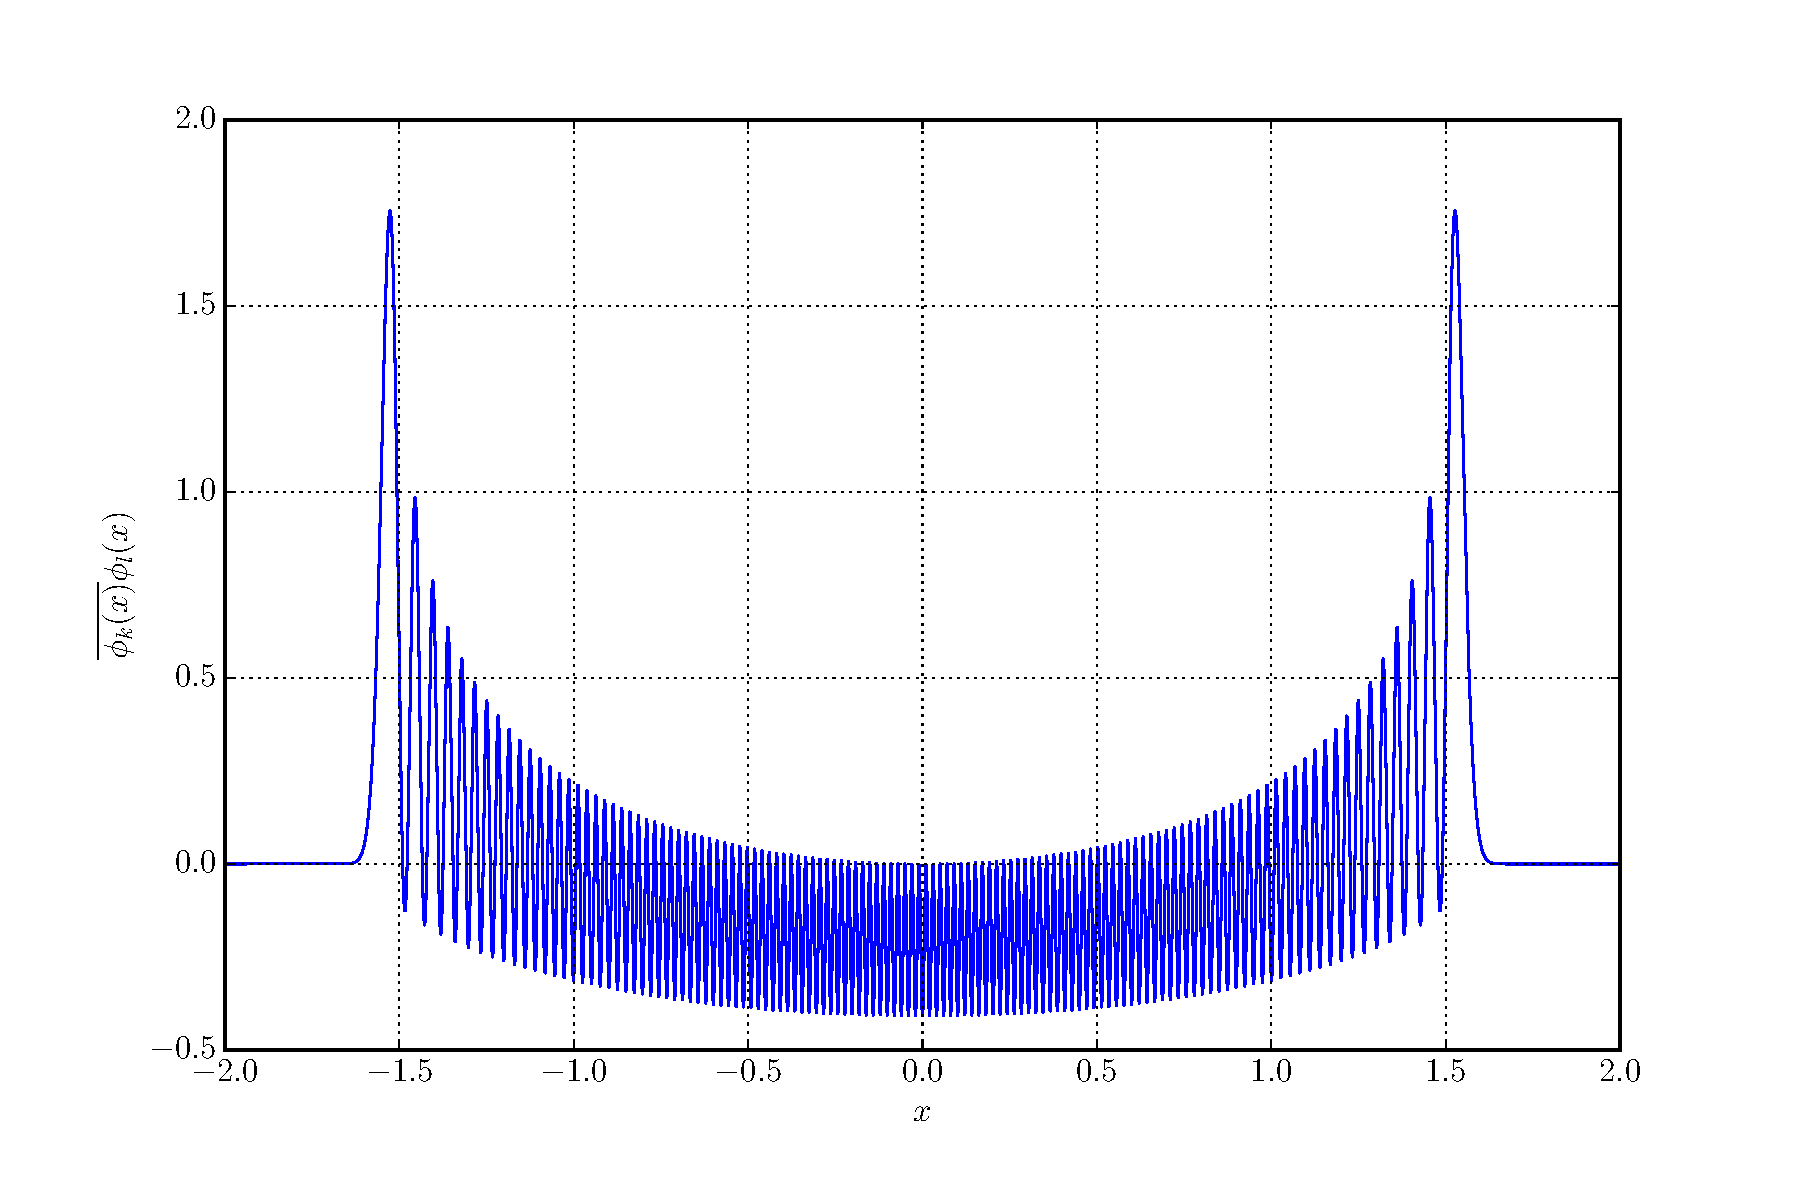
\includegraphics[width=0.8\linewidth]{./fig/poly_oscillations.pdf}
  \caption{Integrand of the overlap of $\phi_{120}$ and $\phi_{122}$
  with $\varepsilon=0.1$. The parameter set $\Pi = \{0,0,1,\imath\}$
  is identical for both packets and hence the exponential parts cancel
  to $\exp(-\frac{x^2}{\varepsilon^2})$. This example shows the oscillatory
  structure caused solely by the high degree of the polynomials involved.}
  \label{fig:polynomials_oscillations}
\end{figure}

In the end, the values $k$ and $l$ set the lower bound on the number of Gauss-Hermite
quadrature nodes that we have to use for correct integration. This is very unfortunate
and can diminish the gain in number of nodes obtained through the steepest descent
transformation. However, with modern algorithms it is easily possible to compute
Gaussian quadrature with hundreds or even thousands of quadrature points~\cite{GLR,TTS}.
This makes the problem accessible for direct computation. Some work in this direction
will be shown in a future report.

One might try to resolve these oscillations by another method on top
of what we did so far. Rewriting the Hermite polynomials into their integral formulation
\begin{equation*}
  \operatorname{H}_n(x) =
  \frac{\exp\left(\frac{3\pi \imath n}{2}\right) 2^n}{\sqrt{\pi}}
  \int_{-\infty}^{\infty} t^n e^{-{(t - \imath x)}^2} \di{t}
\end{equation*}
does not solve the problem as there is still a troublesome factor $t^n$.
If we would apply the steepest descent transformation to this integral, computing
the $n$-th power of the integration paths will again yield polynomials of high order.

The next open problem is about integrals $\braket{\phi|\hat{o}|\phi}$ including
additional scalar multiplicative or differential operators $\hat{o}$. An example
of this kind is the computation of expectation values of potential\footnote{Kinetic energy
expectation $\braket{\phi|\hat{T}|\phi}$ is in our case no issue because the
gradient of a wavepacket can be expressed in a linear combination of new wavepackets
again, hence we are back at the case $\braket{\phi_k|\phi_l}$.}
energies: $\braket{\phi|V|\phi}$.
In this example given, the same wavepacket $\phi$ appears in both, the bra and the
ket part of the integral. Therefore the integration is much easier, oscillations
caused by the exponential parts cancel out to a large degree. But let us consider
the general case where we have $\braket{\phi|\hat{o}|\phi^\prime}$. The main issue
here are the possible effects on the oscillator $g$ induced by $\hat{o}$. For example,
assume that $\hat{o}$ is a potential $V(x)$. Then, $V$ becomes part of the envelope
and there apply some growth limits on the envelope $f$ for $|x| \rightarrow \infty$.
If $V$ contains exponential parts, they have to be merged into the oscillator $g$ and
in turn change the integration paths. Further, if there are any poles
in $f$, we have to be very careful with integration too and make sure to include all
the relevant residuals. In the computations done so far, the envelope $f$ is assumed
to have no poles in $\mathbb{C}^{N}$. Altogether this poses some challenges for
non-polynomial potentials. Polynomial potentials are tame enough to
fit the framework shown.

Although there are some loose ends, we have constructed a method which works better
for larger $\omega$ hence for smaller semiclassical scaling $\varepsilon$.
It gives excellent results in the interesting and complicated case where
$\Pi \approx \Pi^{\prime}$.


\section{Numerical Examples}

\subsection{Motivation}


The initial motivation for this research originates from the computation of autocorrelations
of wavepackets $\Psi$ like:
\begin{equation}\label{eq:compute_ac_wavepackets}
  I = \Braket{\Psi[\Pi] | \Psi[\Pi^{\prime}]}
    = \idotsint_{\mathbb{R}^{D}} \conj{\Psi[\Pi]} \Psi[\Pi^{\prime}] \mathrm{d}\vec{x} \,.
\end{equation}


This turns out to be very challenging. In some of the most interesting cases where
$\Pi \approx \Pi^{\prime}$ holds or where the semiclassical scaling parameter $\varepsilon$
becomes small, Gaussian quadrature introduces huge errors and hence we find spurious
non-physical correlations.

For example we studied the time-dependent Schr\"odinger equation with a wave\-packet $\Psi$
propagating in a Morse potential $V(x)$. The potential was fit to experimental data which
are taken from~\cite{SIZ_hg2}. The semiclassical scaling parameter $\varepsilon = 0.048360$
representing mass ratio between nuclei and electrons matches the nuclear dynamics of the
mercury compound \ce{Hg2}.

\begin{figure}
  \centering
  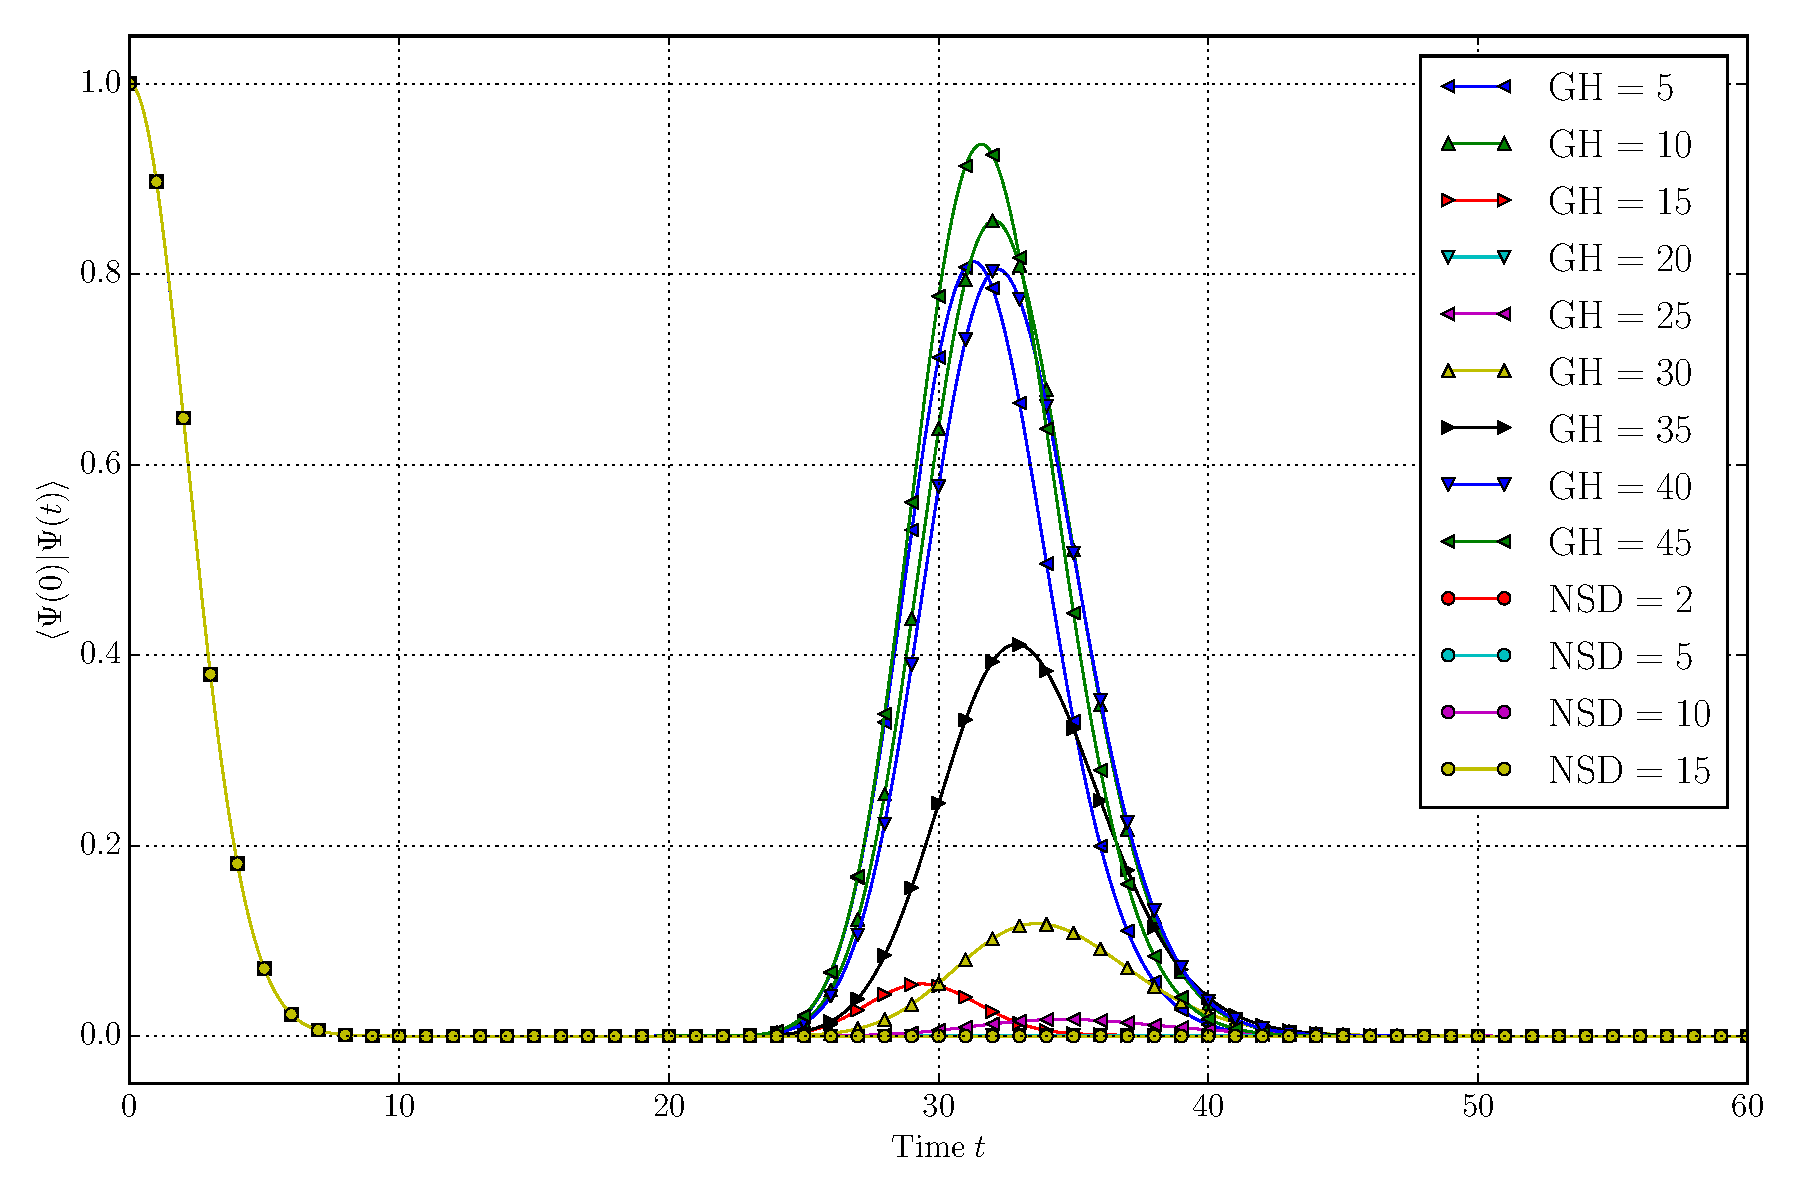
\includegraphics[width=0.8\linewidth]{./fig/ac_mercurial_morse.pdf}
  \caption{Autocorrelation of the Mercury dynamics computed with classical
  Gauss-Hermite quadrature and with the steepest descent method each with several
  numbers of quadrature points. While Gauss-Hermite quadrature fails,
  the numerical steepest descent transformation yields accurate results.}
  \label{fig:ac_mercurial_morse}
\end{figure}

Gauss-Hermite quadrature with any number of nodes shows high spurious autocorrelation bumps,
compare to Figure~\ref{fig:ac_mercurial_morse}. Using the steepest descent transformation
before applying a quadrature scheme gives correct results for an even smaller number of nodes.

In the following we will perform a number of different numerical simulations and show
the robustness as well as pleasant convergence properties of this new technique.
All simulations shown here were carried out by our implementation in the \texttt{WaveBlocks}
simulation code~\cite{waveblocksnd}.


\subsection{Two-Packet Experiment}


In this section we show the insufficiency of the Gauss-Hermite quadrature
for computing the integral in~\eqref{eq:compute_ac_wavepackets}. The setup
of this experiment consists of two wavepackets $\phi[\Pi]$ and $\phi[\Pi^\prime]$.
Both are fixed in space at positions $q$ and $q^\prime$. Next we direct the
momenta $p$ and $p^\prime$ towards each other ($p^\prime = -p$) and start
increasing their magnitude $|p|$. (Note that for all figures below, the values
of the $p$ axis are multiplicative factors on top of the wavepacket' original
values $p$ and $p^\prime$.)
The procedure is shown also in Figure~\ref{fig:convergence_setup}.

\begin{figure}[h!]
  \centering
  \includegraphics[width=0.5\linewidth]{./fig/convergence_setup.pdf}
  \caption{Setup of the first experiment. There are two wavepackets $\Psi$
    and $\Psi^\prime$ located next to each other at fixed positions $q$ and
    $q^\prime$. We set increasing momenta $p$ and $p^\prime$
    in opposite direction.}
  \label{fig:convergence_setup}
\end{figure}

The higher the momenta, the more oscillations appear in the product $\conj{\phi}(x) \phi^\prime(x)$.
These oscillations are difficult for Gauss Hermite quadrature to catch and accuracy
will break down even for relatively small momenta. On the other hand, since the
steepest descent transformation applies to arbitrary high oscillator frequency,
it perfectly handles arbitrary momenta and converges fast to the correct
overlap integral value.

For the one-dimensional case there exists an analytic formula for computing
the integral for any state $\phi_k$. Evaluation is very expensive but can nevertheless
serve as exact reference solution. For examples in higher dimensions we can take
the formula for general Gaussian integrals in case we look at ground states
$\phi_{\vec{0}}$ only. Otherwise we take the computation including the steepest
descent transformation using the largest number of quadrature nodes as reference.

The whole process of computing the integral works as shown in the
Figure~\ref{fig:transformation_chain_2}. Especially in the multi-dimensional case
we still need a full tensor product of $N$ Gauss-Hermite quadrature nodes in the end.
This results in $N^D$ quadrature nodes, which scales exponentially with the
dimension $D$. The important bit is however that the value of $N$ is \emph{much}
smaller compared to direct application of traditional quadrature schemes as done
in~\ref{fig:transformation_chain_1}.
The only oscillations that remain are caused by the degree of the polynomial part
of the integrand for large state index $k$. There, the order bounds of Gauss
quadrature of course still apply.

\FloatBarrier
\subsubsection{Convergence in $|p|$}


\begin{figure}[ht!]
  \begin{subfigure}[t]{0.5\linewidth}
    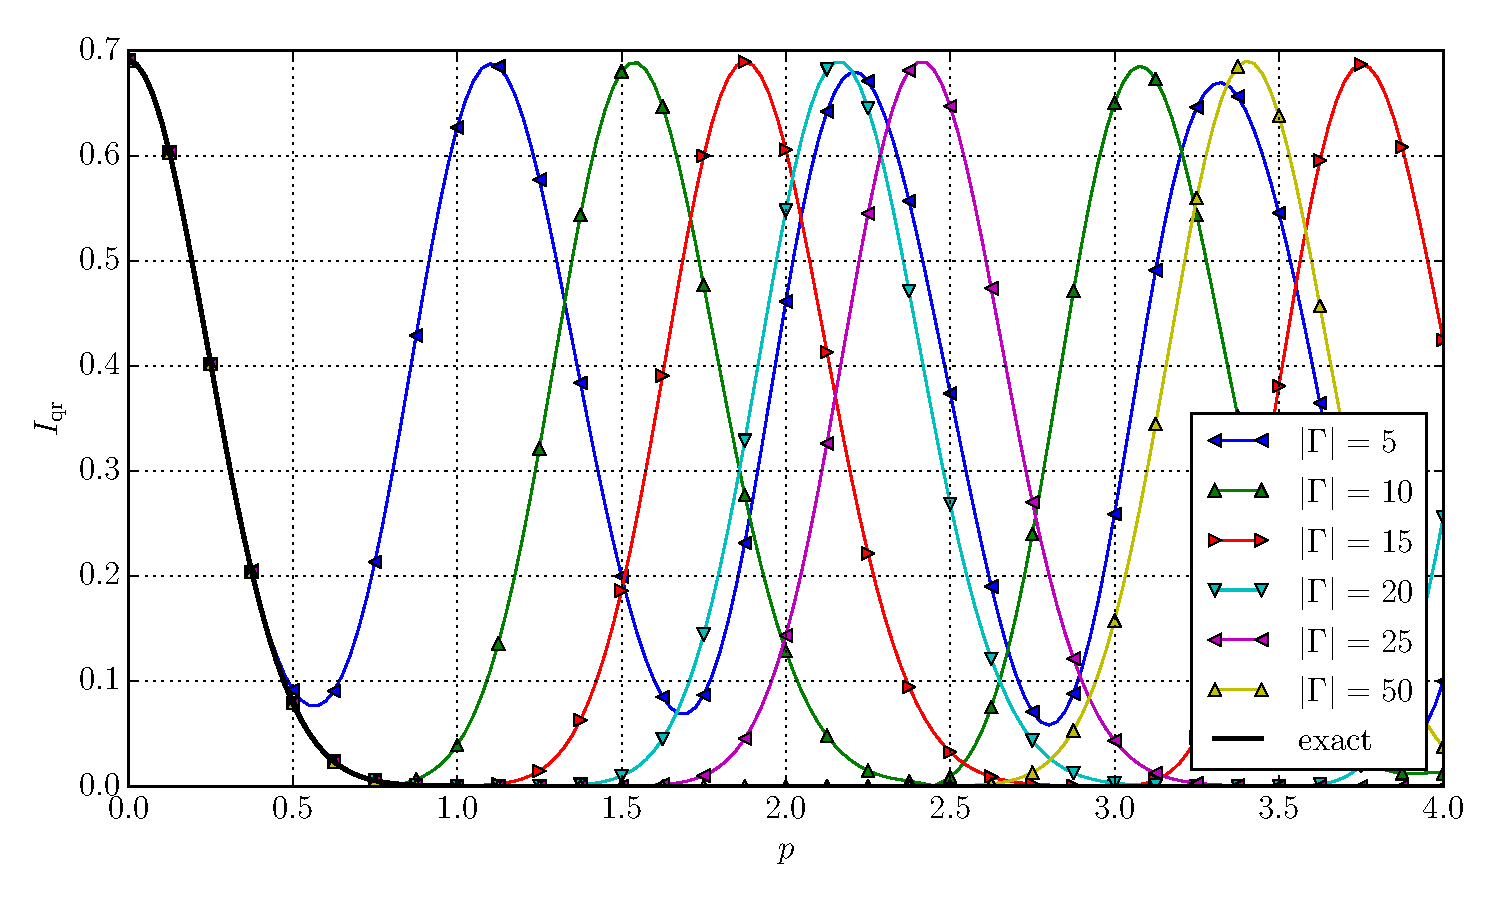
\includegraphics[width=\linewidth]{./plots/tp_1d_conv_p_0_0_val_qr.pdf}
    \caption{Direct Gauss-Hermite quadrature of size $N$ with a total of $|\Gamma|$ nodes.}
    \label{fig:tp_1d_conv_p_0_0_val_qr}
  \end{subfigure}
  \begin{subfigure}[t]{0.5\linewidth}
    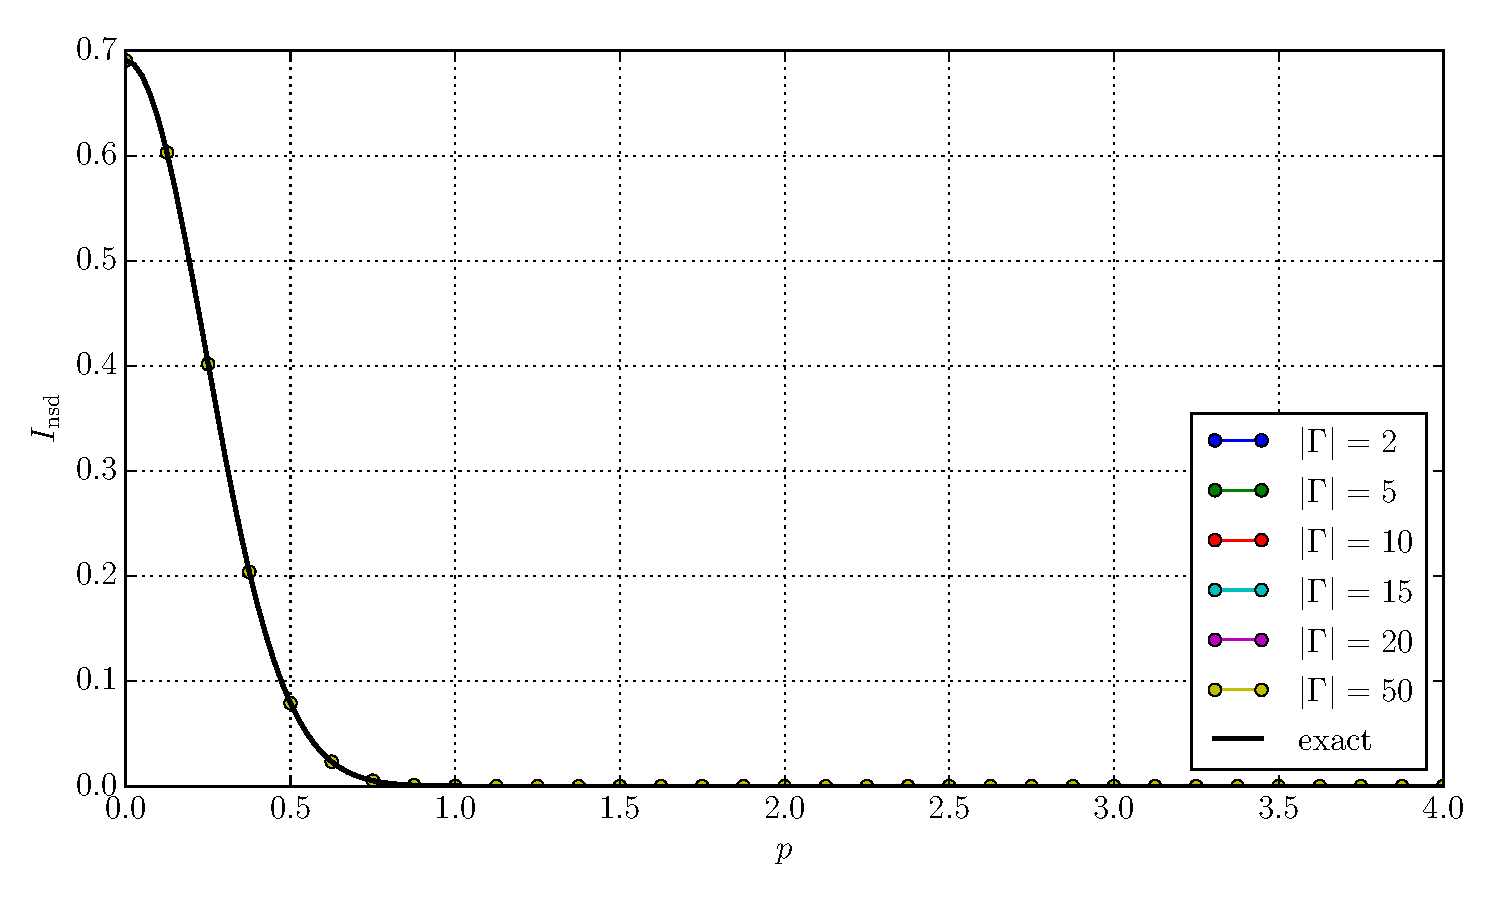
\includegraphics[width=\linewidth]{./plots/tp_1d_conv_p_0_0_val_nsd.pdf}
    \caption{Steepest descent transformation and Gauss-Hermite quadrature of size $N$ with a total of $|\Gamma|$ nodes.}
    \label{fig:tp_1d_conv_p_0_0_val_nsd}
  \end{subfigure} \\
  \begin{subfigure}[t]{0.5\linewidth}
    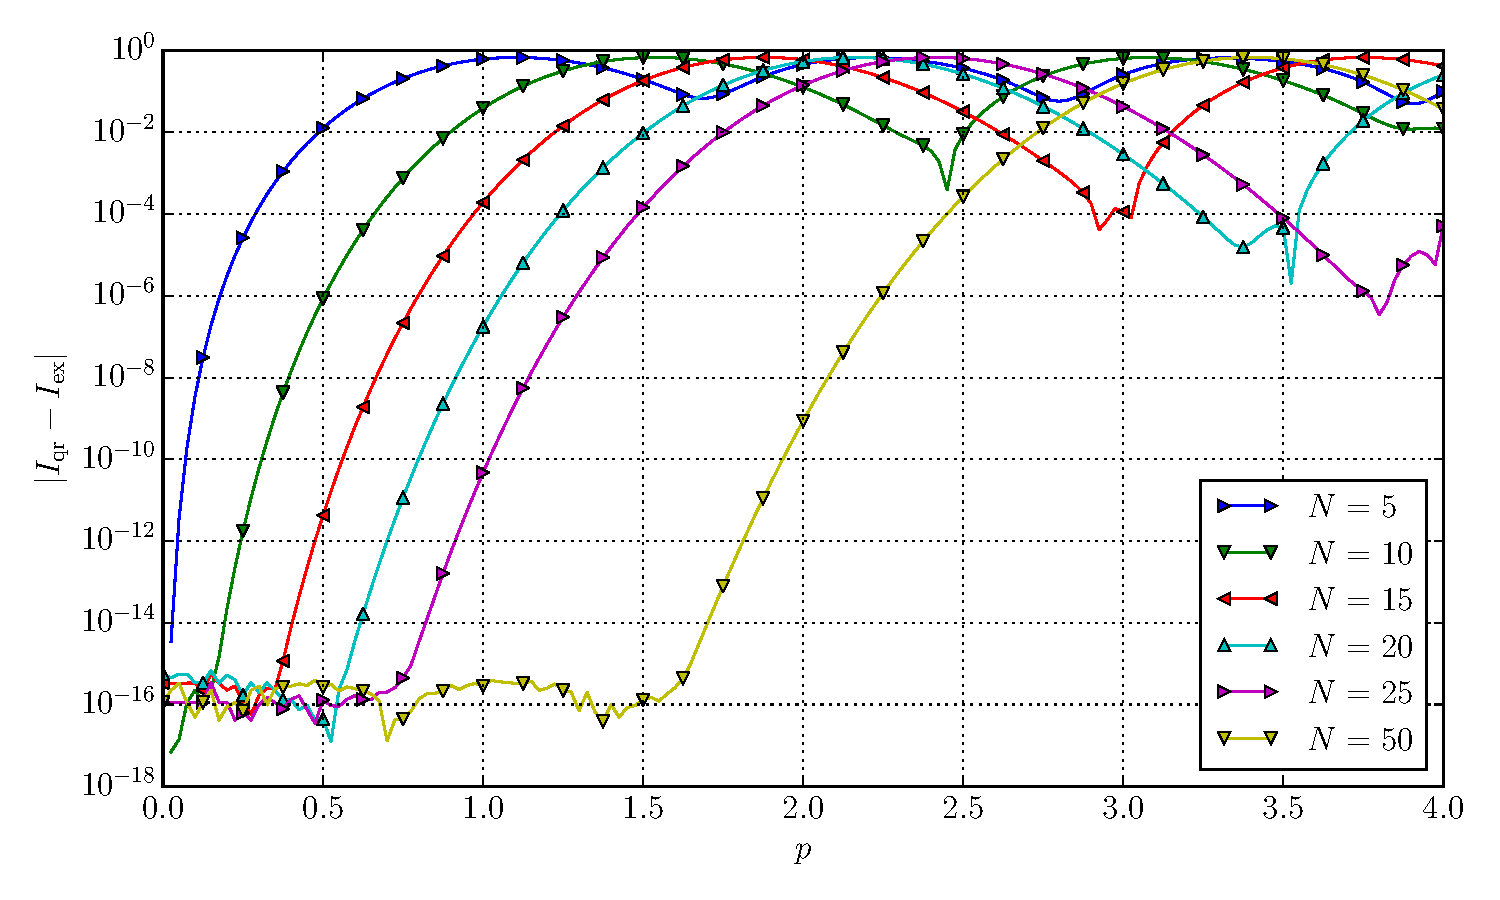
\includegraphics[width=\linewidth]{./plots/tp_1d_conv_p_0_0_err_qr.pdf}
    \caption{Absolute error of the direct quadrature method compared to the exact solution.}
    \label{fig:tp_1d_conv_p_0_0_err_qr}
  \end{subfigure}
  \begin{subfigure}[t]{0.5\linewidth}
    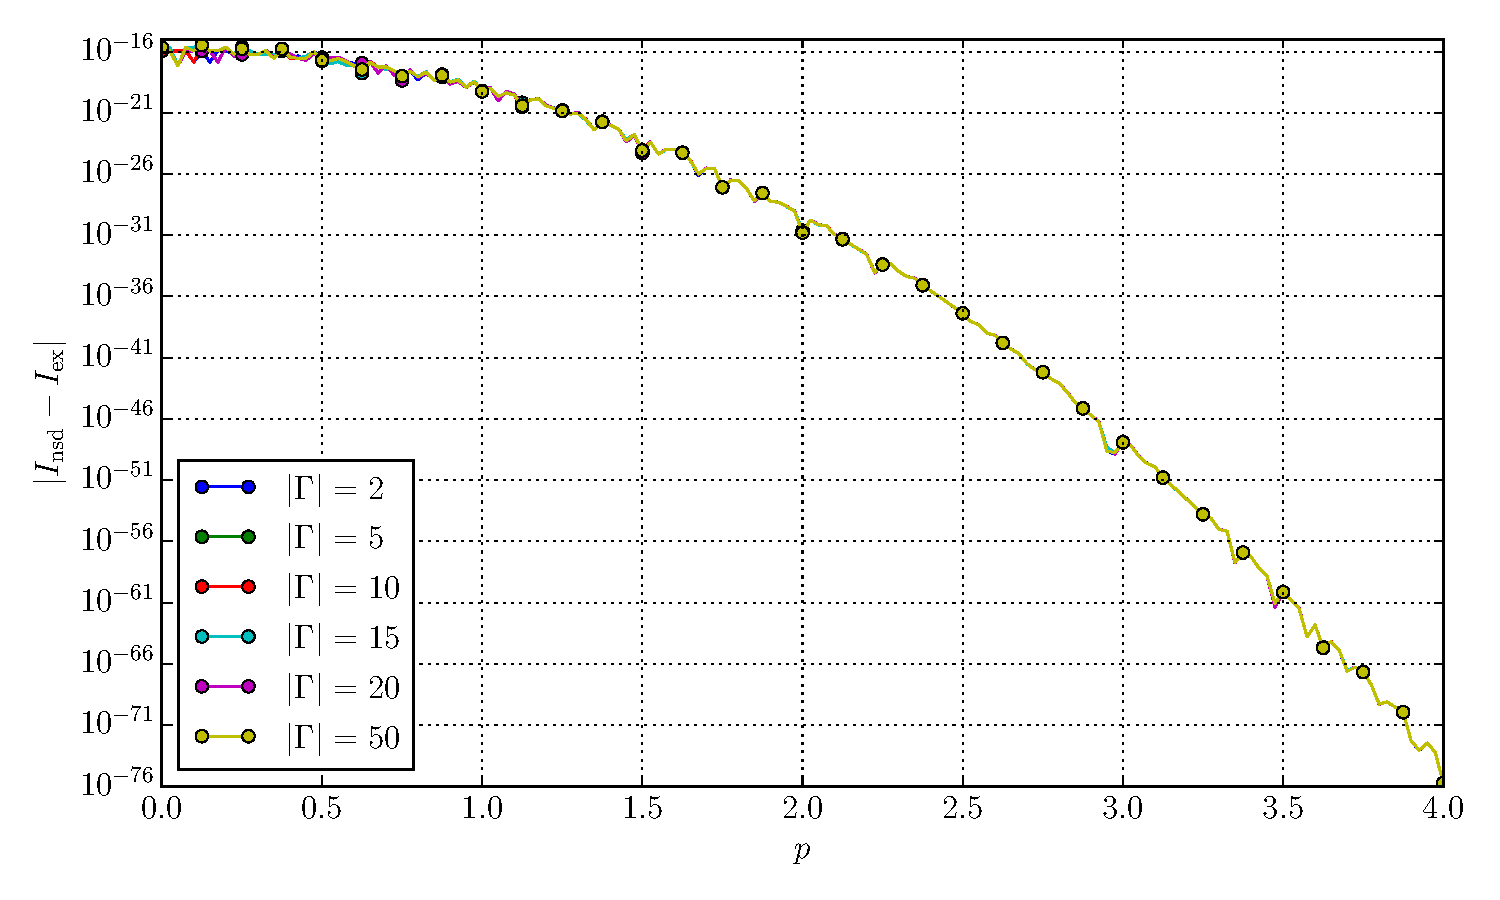
\includegraphics[width=\linewidth]{./plots/tp_1d_conv_p_0_0_err_nsd.pdf}
    \caption{Absolute error of the steepest descent method compared to the exact solution.}
    \label{fig:tp_1d_conv_p_0_0_err_nsd}
  \end{subfigure}
  \begin{subfigure}[t]{0.5\linewidth}
    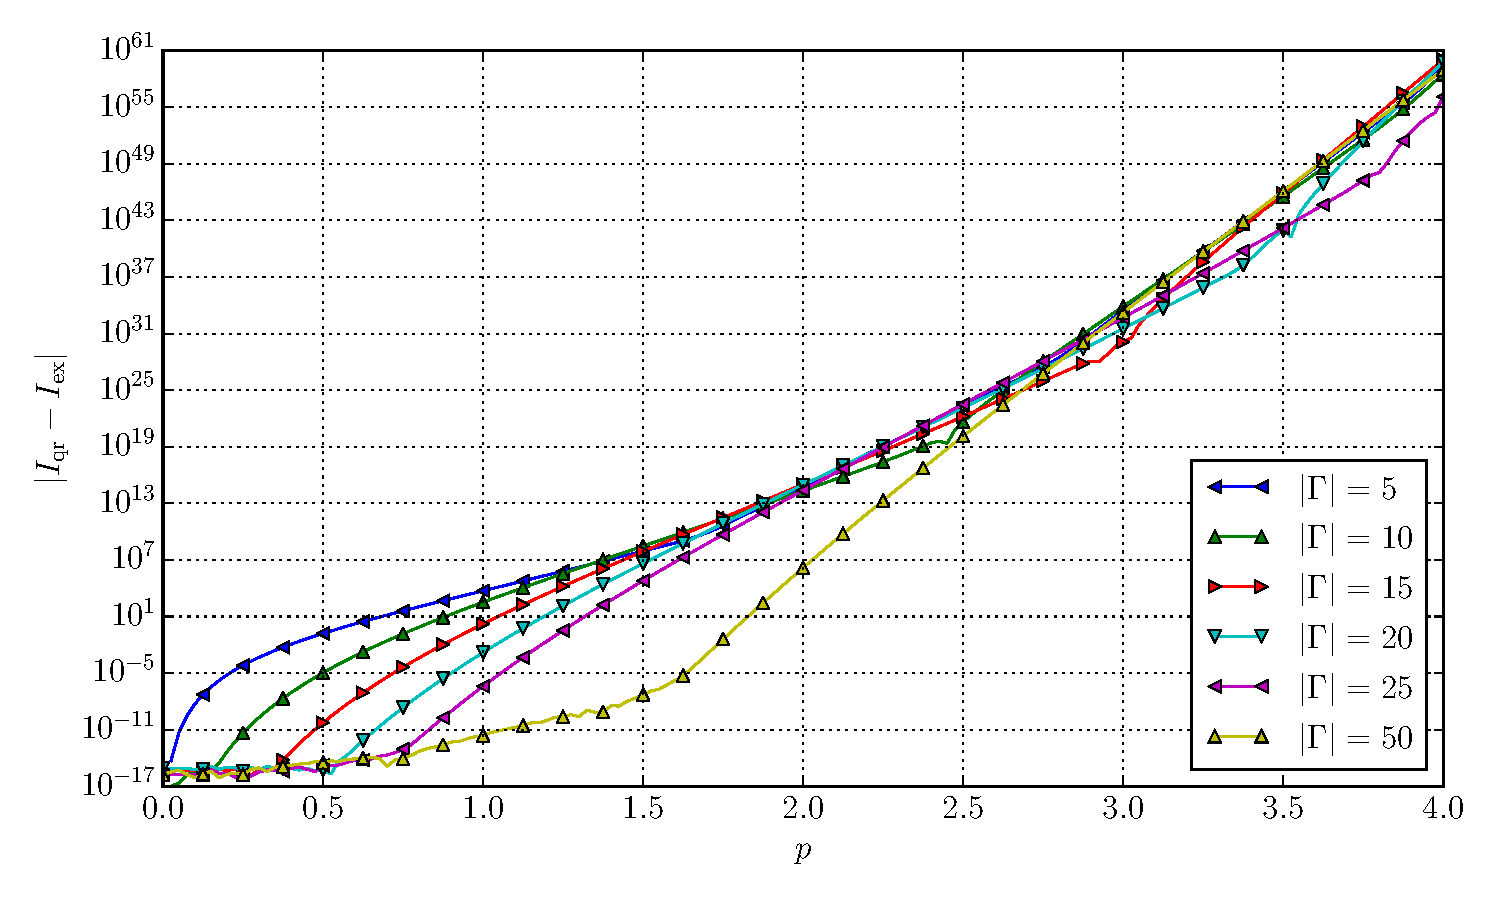
\includegraphics[width=\linewidth]{./plots/tp_1d_conv_p_0_0_err_rel_qr.pdf}
    \caption{Relative error of the direct quadrature method compared to the exact solution.}
    \label{fig:tp_1d_conv_p_0_0_err_rel_qr}
  \end{subfigure}
  \begin{subfigure}[t]{0.5\linewidth}
    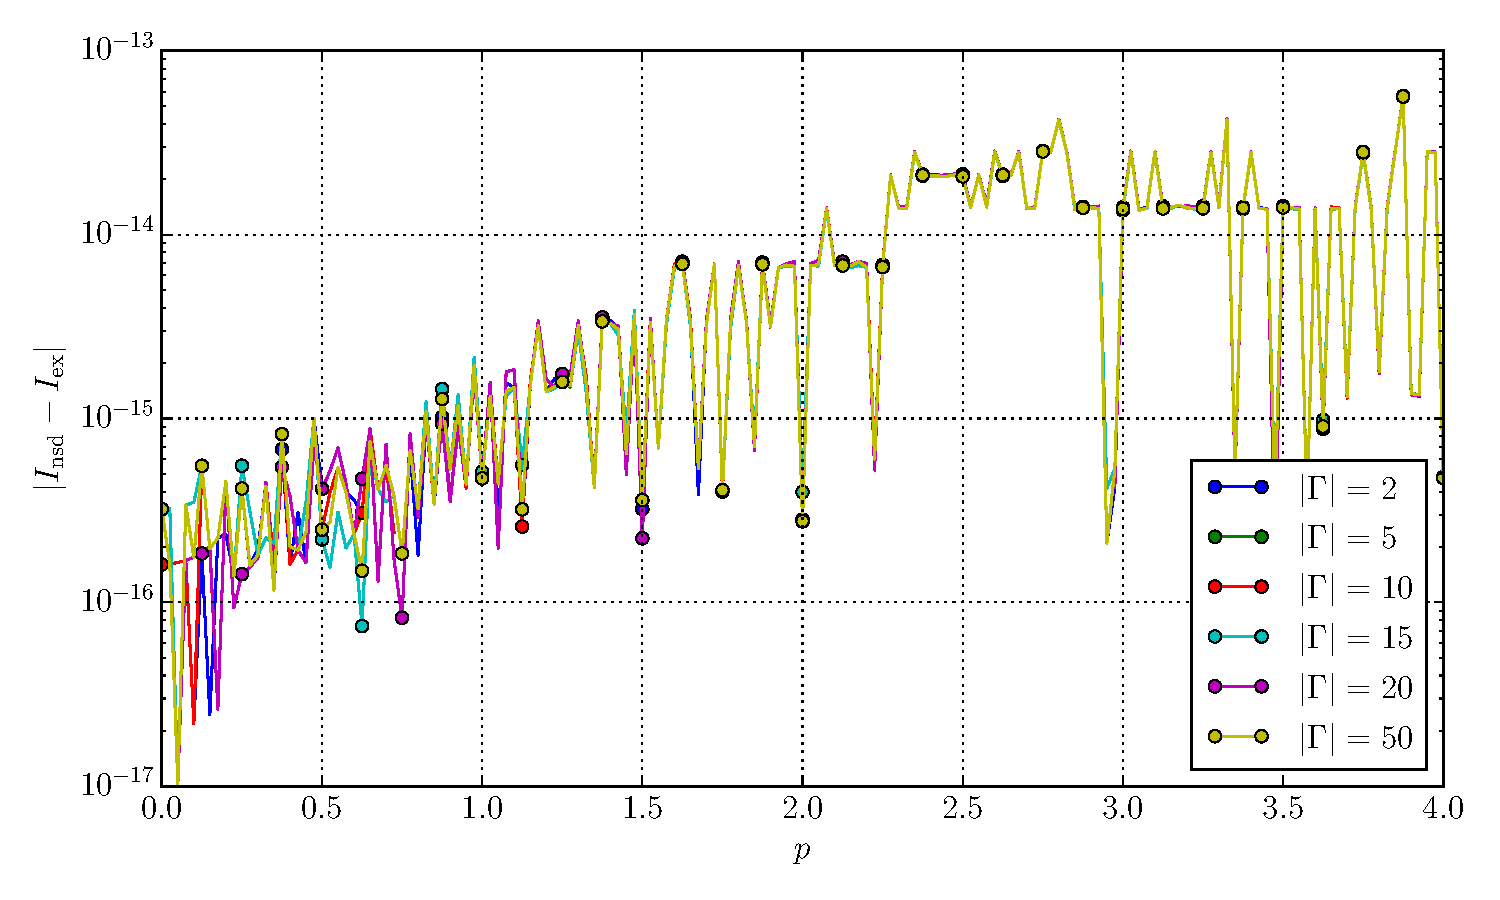
\includegraphics[width=\linewidth]{./plots/tp_1d_conv_p_0_0_err_rel_nsd.pdf}
    \caption{Relative error of the steepest descent method compared to the exact solution.}
    \label{fig:tp_1d_conv_p_0_0_err_rel_nsd}
  \end{subfigure}
  \label{fig:tp_1d_conv_p_0_0}
  \caption{Experiment with $\phi_{0}$ and $\phi_{0}^{\prime}$.
  The parameters are:
  $q=-0.2$, $p=1.5$, $Q=1.0$, $P=1.0\imath$ and
  $q^\prime=0.125$, $p^\prime=-1.5$, $Q^\prime=0.8$, $P^\prime=1.25\imath$
  with $\varepsilon = 0.3$.}
\end{figure}

\begin{figure}[ht!]
  \begin{subfigure}[t]{0.5\linewidth}
    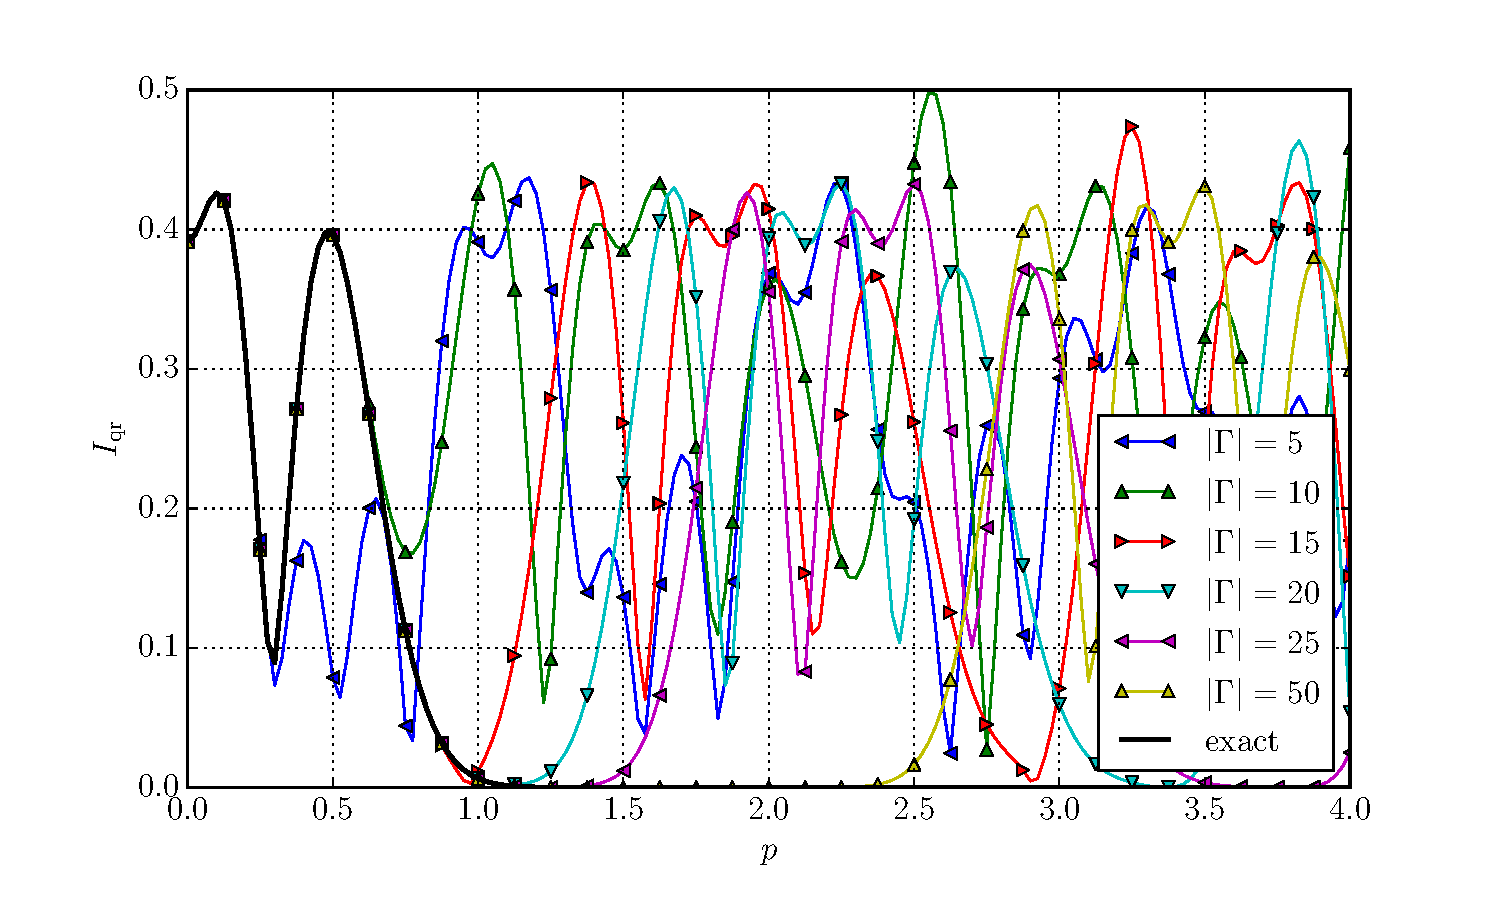
\includegraphics[width=\linewidth]{./plots/tp_1d_conv_p_2_1_val_qr.pdf}
    \caption{Direct Gauss-Hermite quadrature of size $N$ with a total of $|\Gamma|$ nodes.}
    \label{fig:tp_1d_conv_p_2_1_val_qr}
  \end{subfigure}
  \begin{subfigure}[t]{0.5\linewidth}
    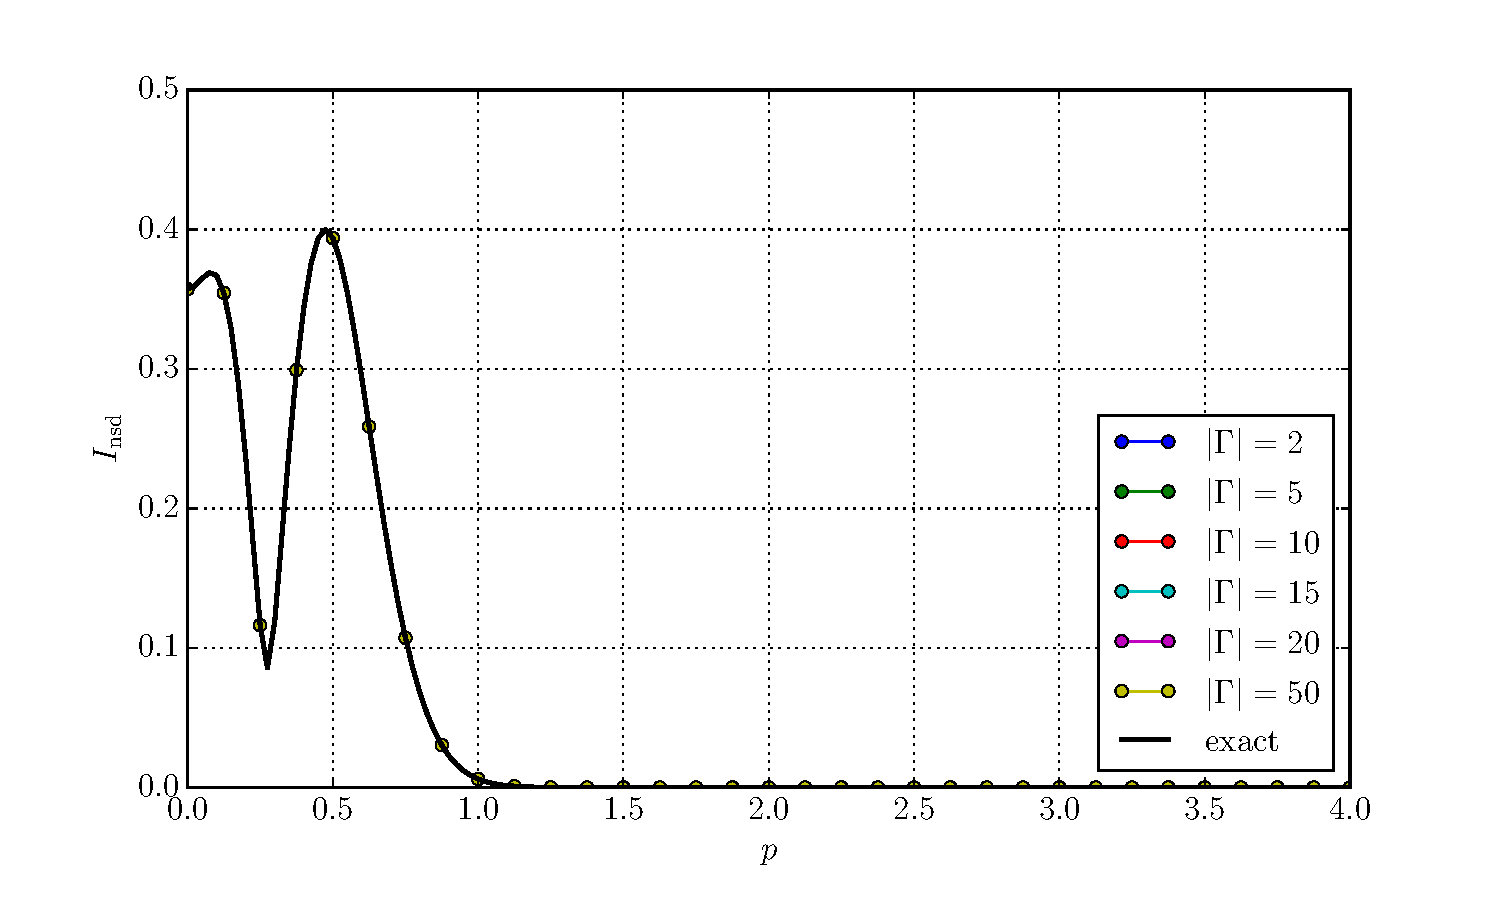
\includegraphics[width=\linewidth]{./plots/tp_1d_conv_p_2_1_val_nsd.pdf}
    \caption{Steepest descent transformation and Gauss-Hermite quadrature of size $N$ with a total of $|\Gamma|$ nodes.}
    \label{fig:tp_1d_conv_p_2_1_val_nsd}
  \end{subfigure} \\
  \begin{subfigure}[t]{0.5\linewidth}
    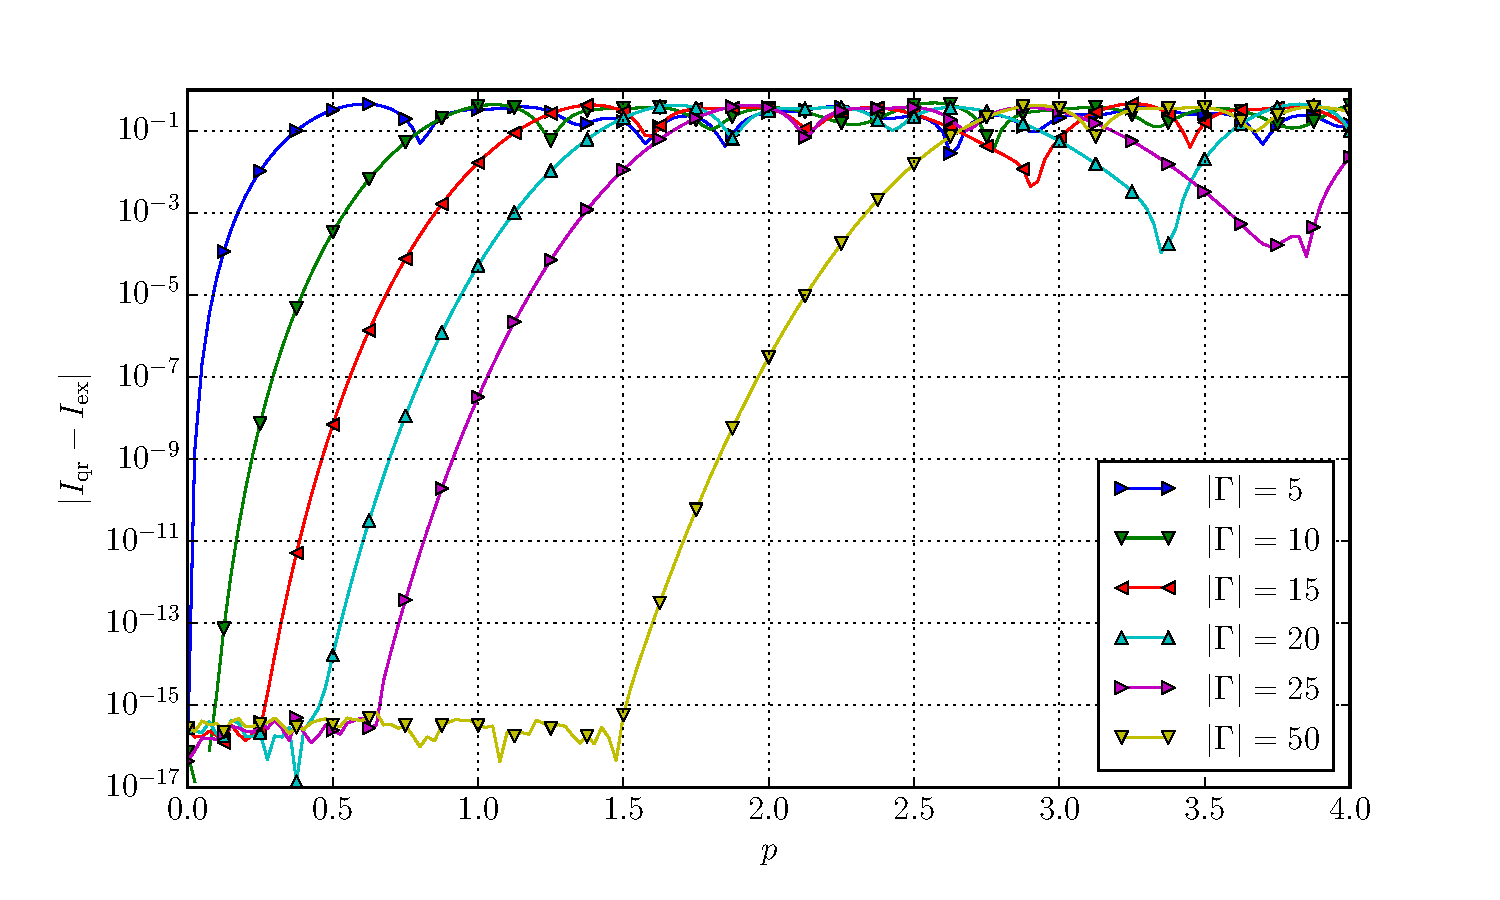
\includegraphics[width=\linewidth]{./plots/tp_1d_conv_p_2_1_err_qr.pdf}
    \caption{Absolute error of the direct quadrature method compared to the exact solution.}
    \label{fig:tp_1d_conv_p_2_1_err_qr}
  \end{subfigure}
  \begin{subfigure}[t]{0.5\linewidth}
    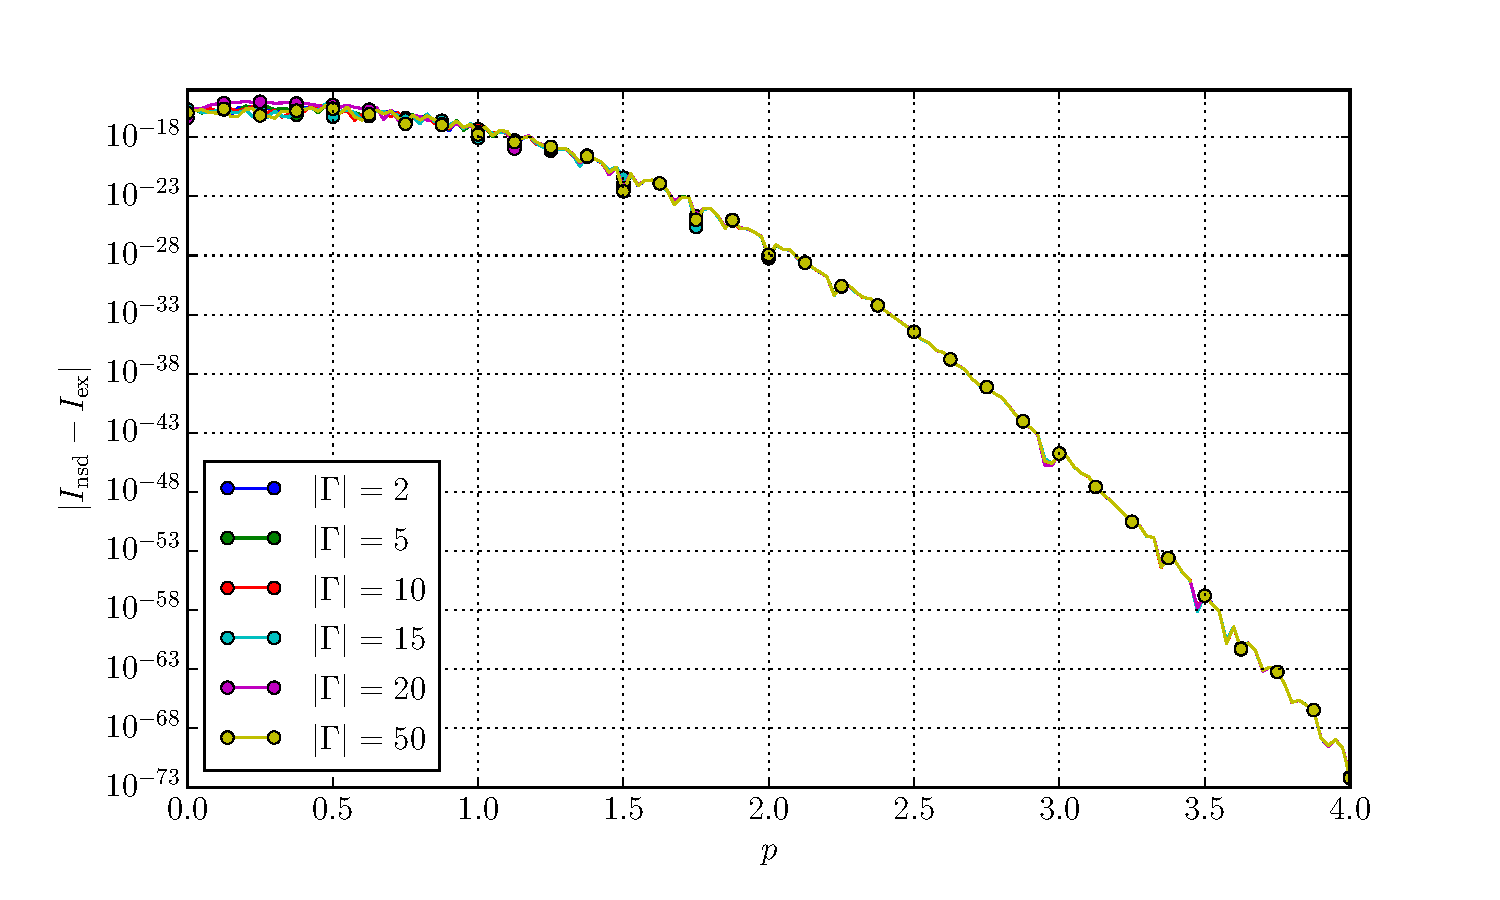
\includegraphics[width=\linewidth]{./plots/tp_1d_conv_p_2_1_err_nsd.pdf}
    \caption{Absolute error of the steepest descent method compared to the exact solution.}
    \label{fig:tp_1d_conv_p_2_1_err_nsd}
  \end{subfigure}
  \begin{subfigure}[t]{0.5\linewidth}
    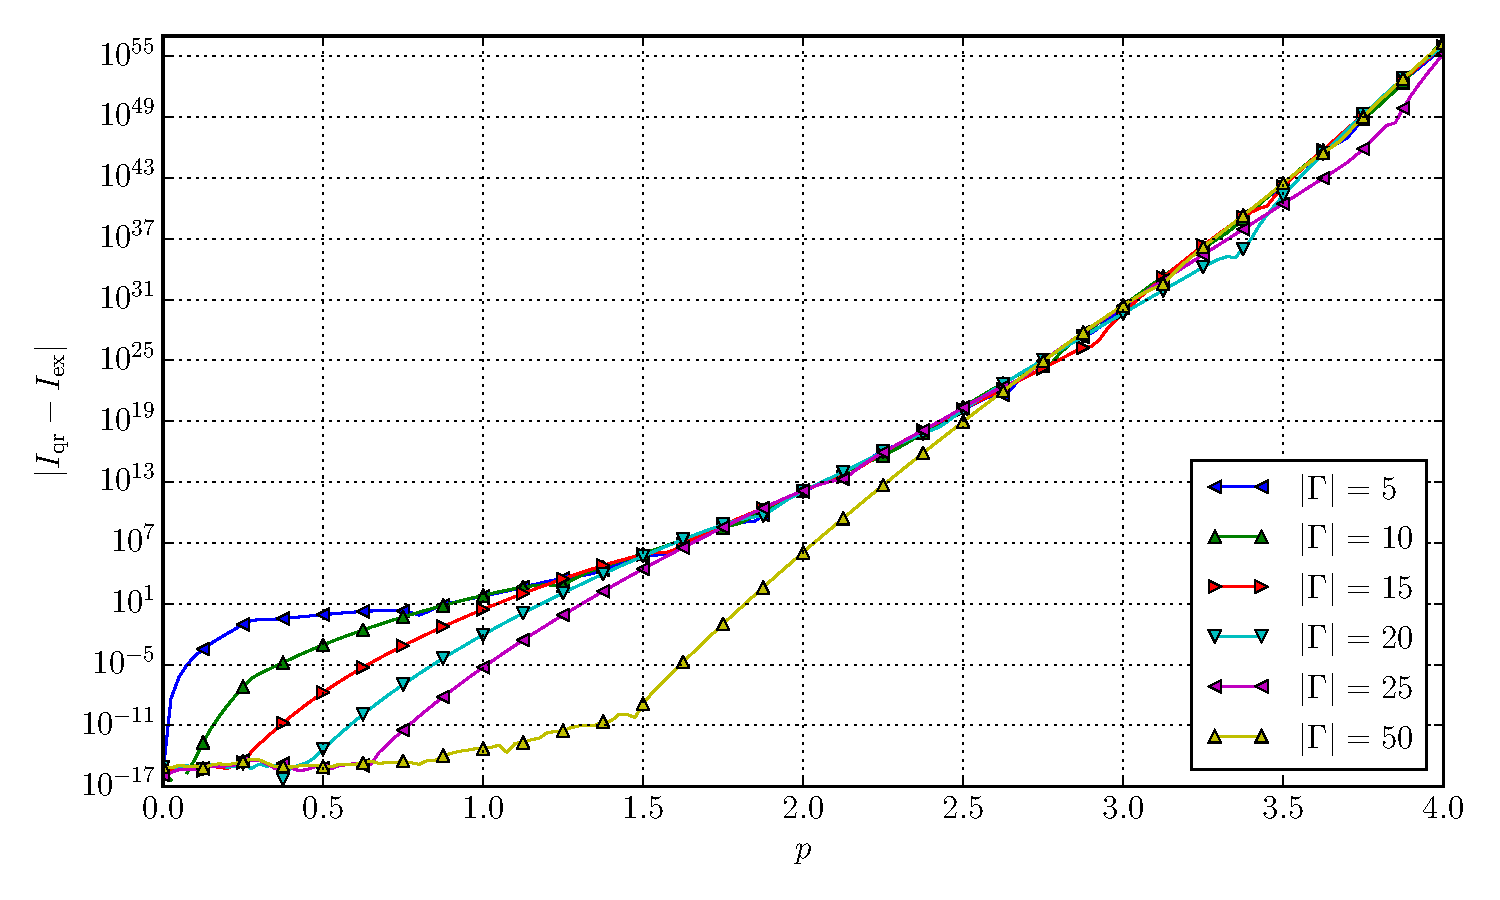
\includegraphics[width=\linewidth]{./plots/tp_1d_conv_p_2_1_err_rel_qr.pdf}
    \caption{Relative error of the direct quadrature method compared to the exact solution.}
    \label{fig:tp_1d_conv_p_2_1_err_rel_qr}
  \end{subfigure}
  \begin{subfigure}[t]{0.5\linewidth}
    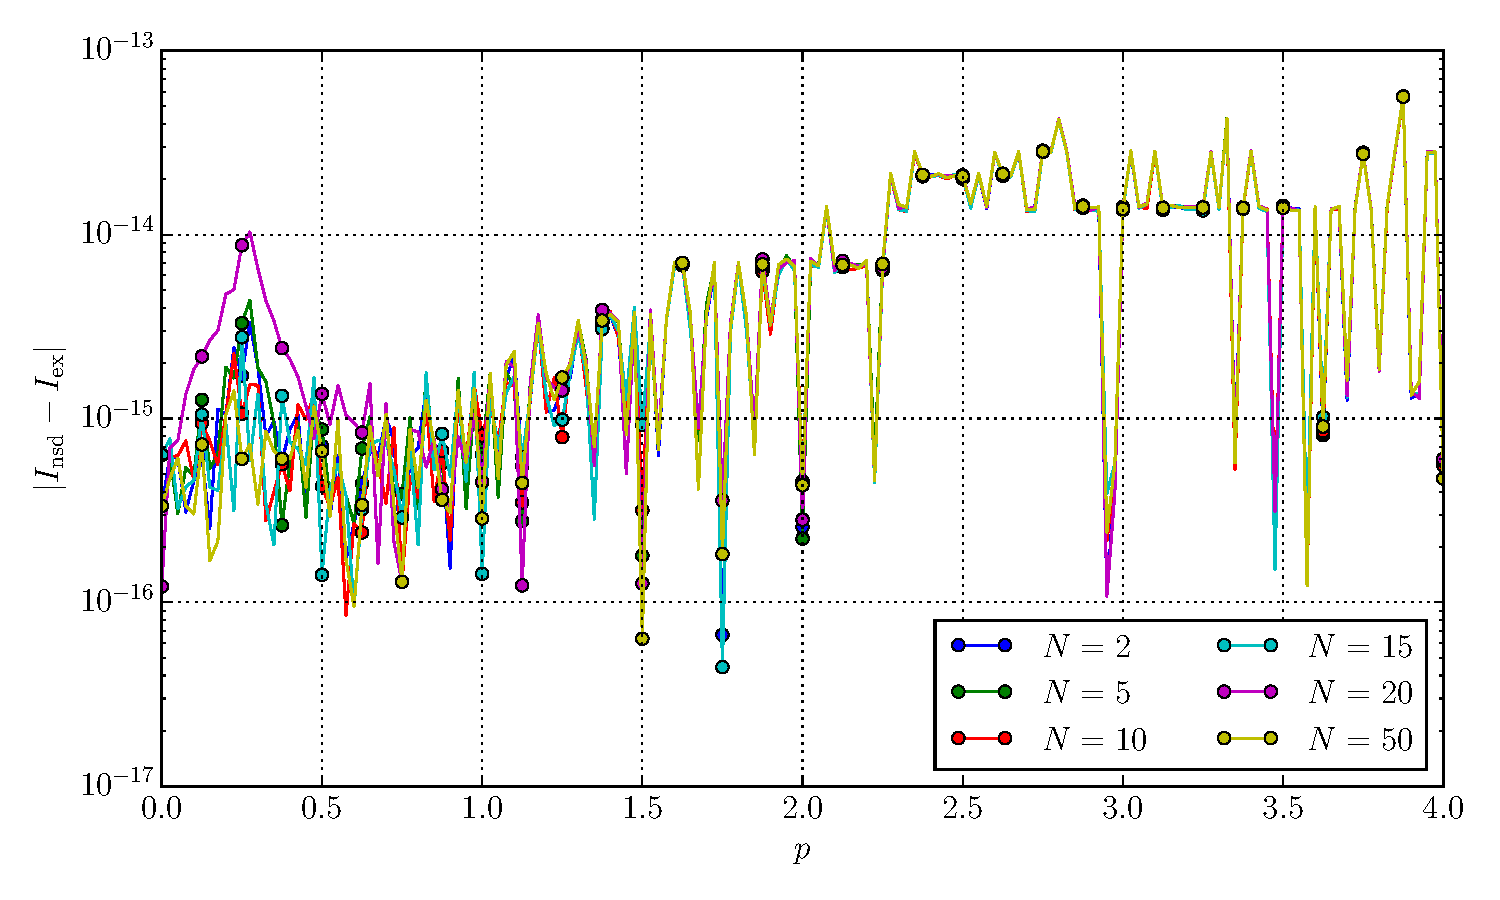
\includegraphics[width=\linewidth]{./plots/tp_1d_conv_p_2_1_err_rel_nsd.pdf}
    \caption{Relative error of the steepest descent method compared to the exact solution.}
    \label{fig:tp_1d_conv_p_2_1_err_rel_nsd}
  \end{subfigure}
  \label{fig:tp_1d_conv_p_2_1}
  \caption{Experiment with $\phi_{2}$ and $\phi_{1}^{\prime}$.
  The parameters are:
  $q=-0.2$, $p=1.5$, $Q=1.0$, $P=1.0\imath$ and
  $q^\prime=0.125$, $p^\prime=-1.5$, $Q^\prime=0.8$, $P^\prime=1.25\imath$
  with $\varepsilon = 0.3$.}
\end{figure}

\begin{figure}[ht!]
  \begin{subfigure}[t]{0.5\linewidth}
    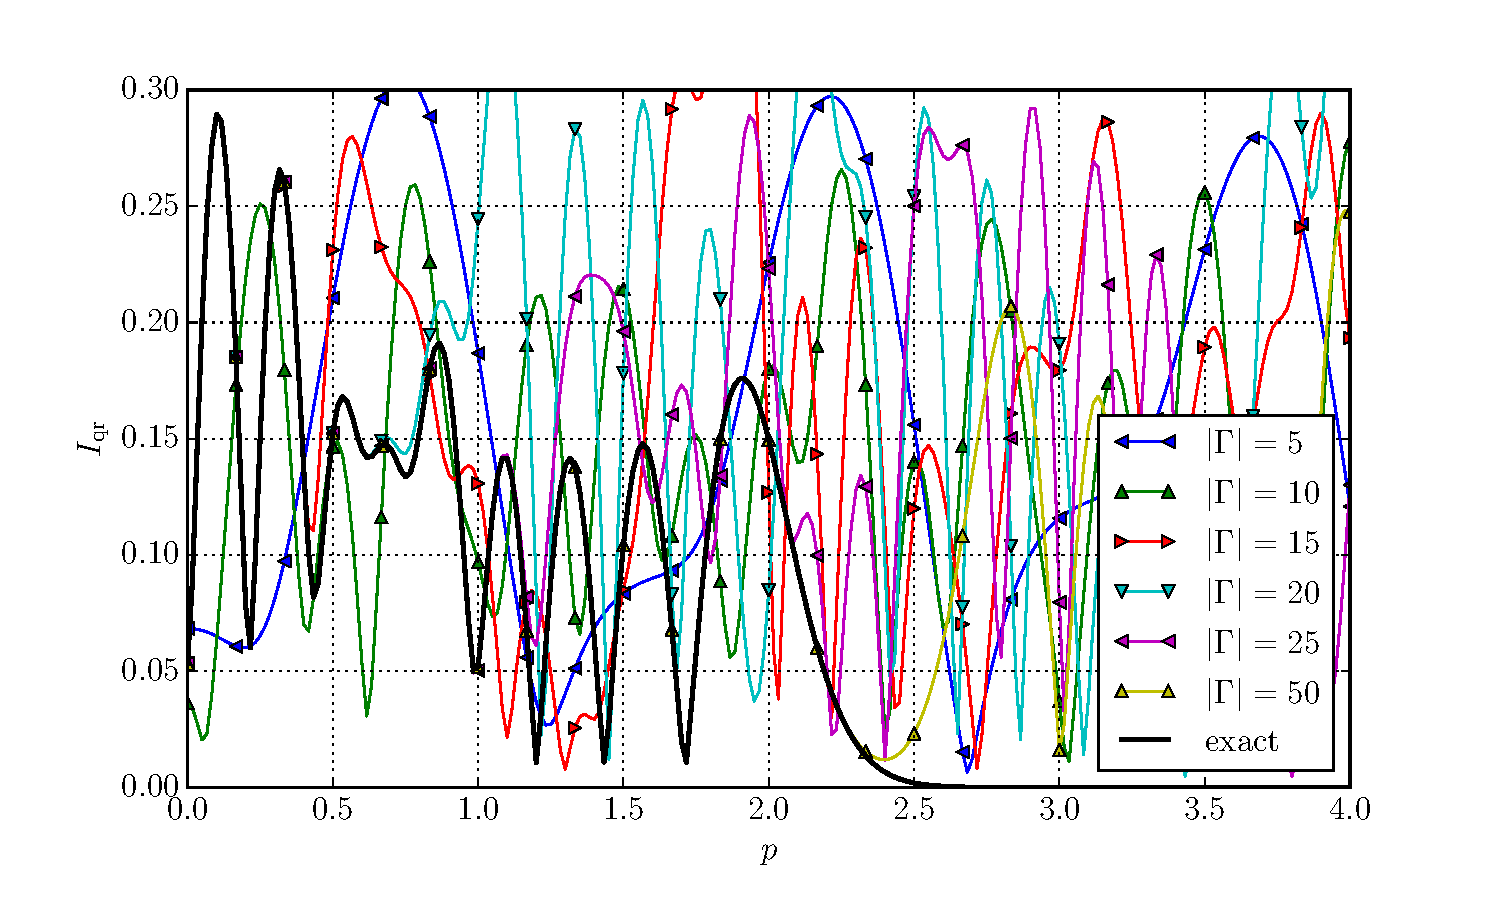
\includegraphics[width=\linewidth]{./plots/tp_1d_conv_p_11_9_val_qr.pdf}
    \caption{Direct Gauss-Hermite quadrature of size $N$ with a total of $|\Gamma|$ nodes.}
    \label{fig:tp_1d_conv_p_11_9_val_qr}
  \end{subfigure}
  \begin{subfigure}[t]{0.5\linewidth}
    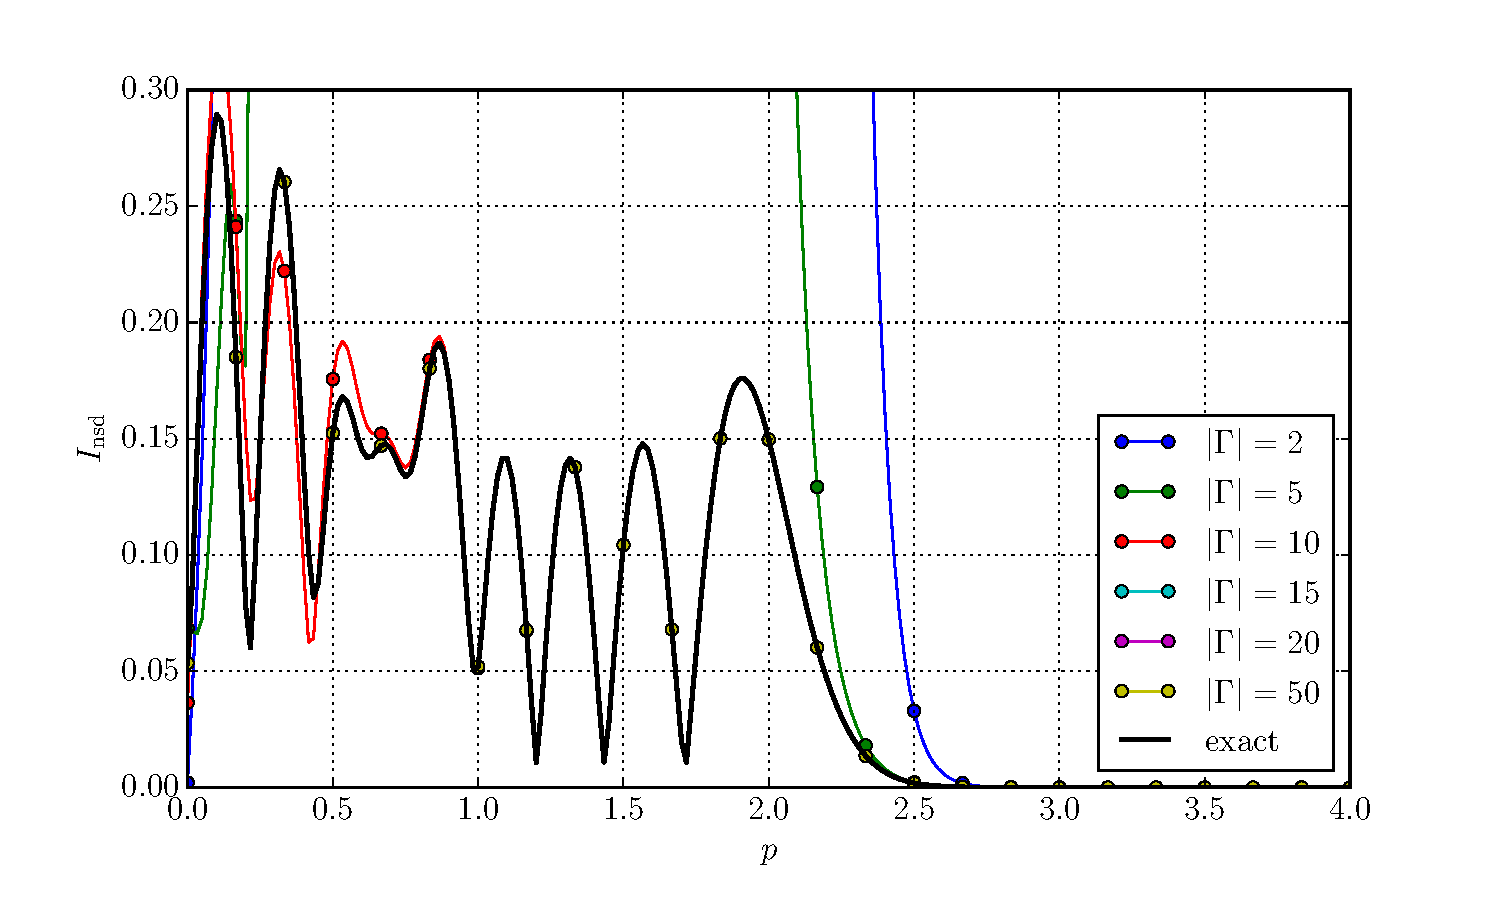
\includegraphics[width=\linewidth]{./plots/tp_1d_conv_p_11_9_val_nsd.pdf}
    \caption{Steepest descent transformation and Gauss-Hermite quadrature of size $N$ with a total of $|\Gamma|$ nodes.}
    \label{fig:tp_1d_conv_p_11_9_val_nsd}
  \end{subfigure} \\
  \begin{subfigure}[t]{0.5\linewidth}
    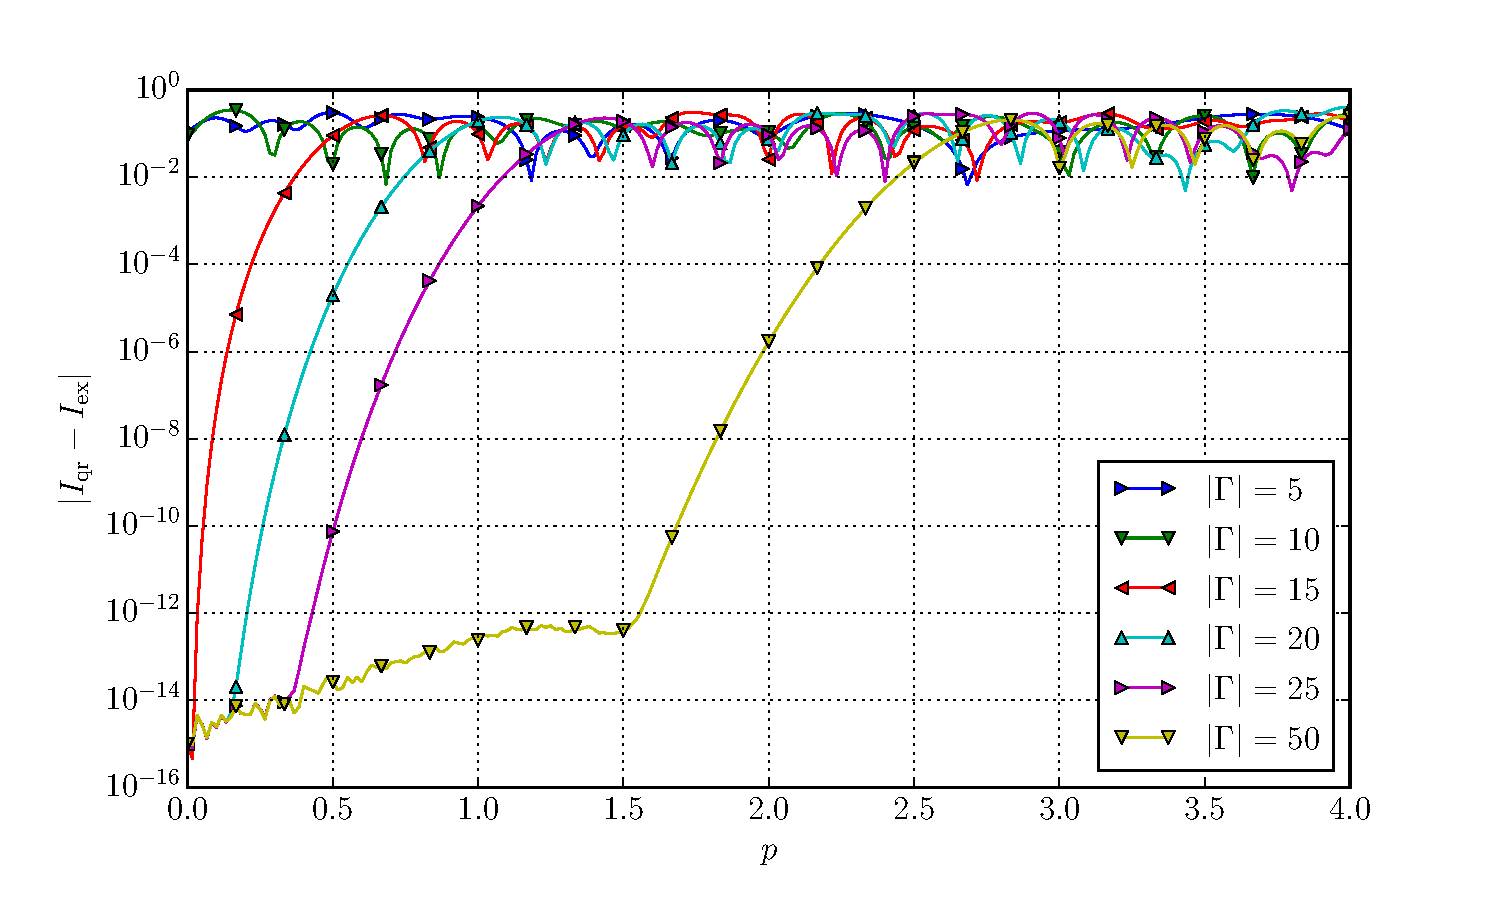
\includegraphics[width=\linewidth]{./plots/tp_1d_conv_p_11_9_err_qr.pdf}
    \caption{Absolute error of the direct quadrature method compared to the exact solution.}
    \label{fig:tp_1d_conv_p_11_9_err_qr}
  \end{subfigure}
  \begin{subfigure}[t]{0.5\linewidth}
    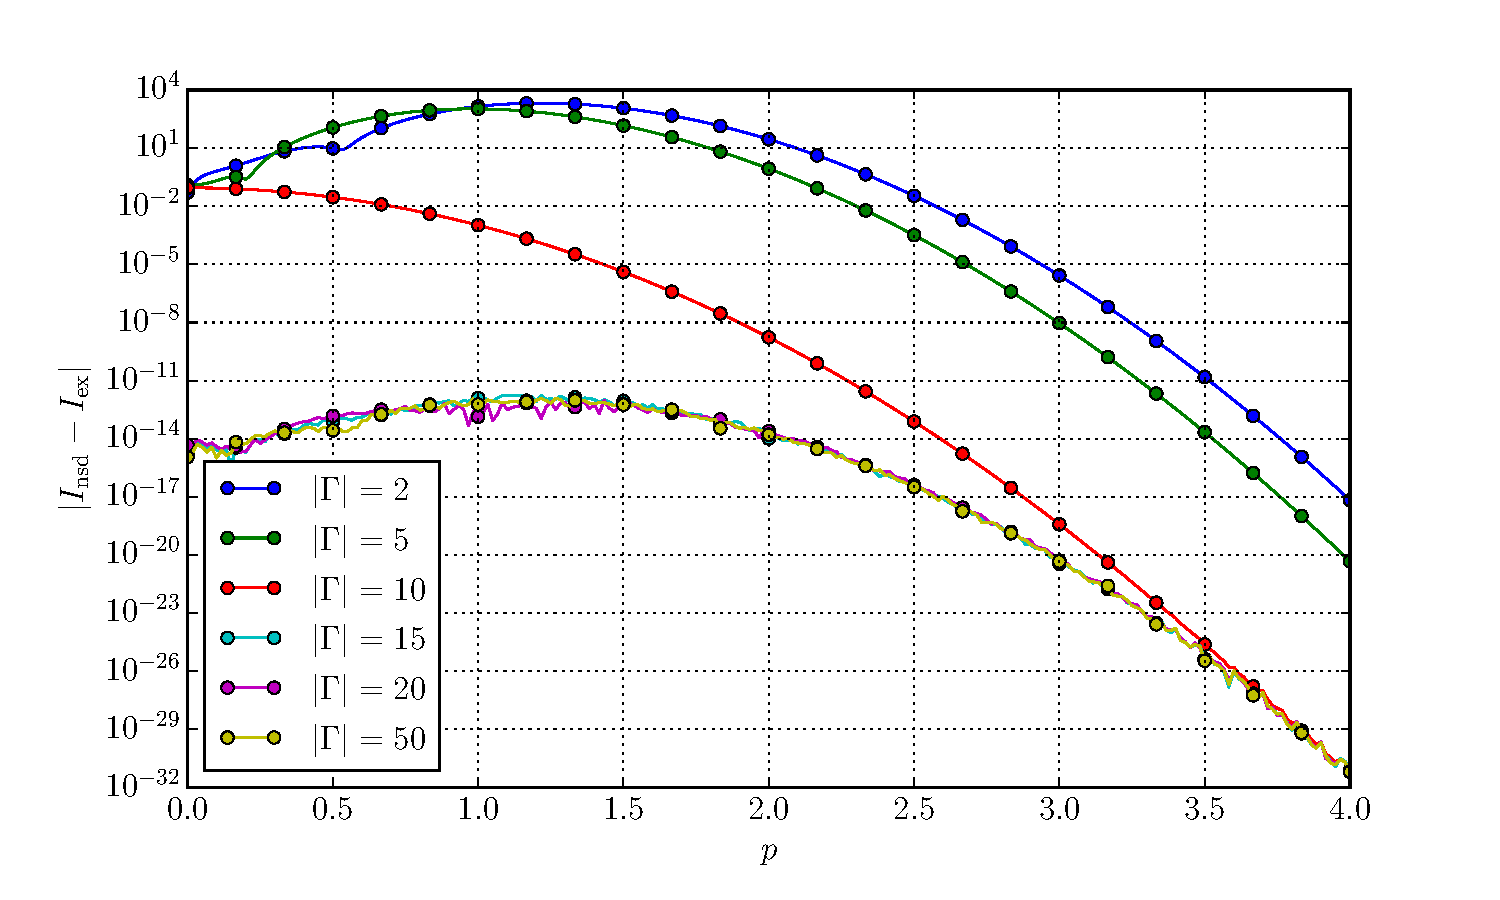
\includegraphics[width=\linewidth]{./plots/tp_1d_conv_p_11_9_err_nsd.pdf}
    \caption{Absolute error of the steepest descent method compared to the exact solution.}
    \label{fig:tp_1d_conv_p_11_9_err_nsd}
  \end{subfigure}
  \begin{subfigure}[t]{0.5\linewidth}
    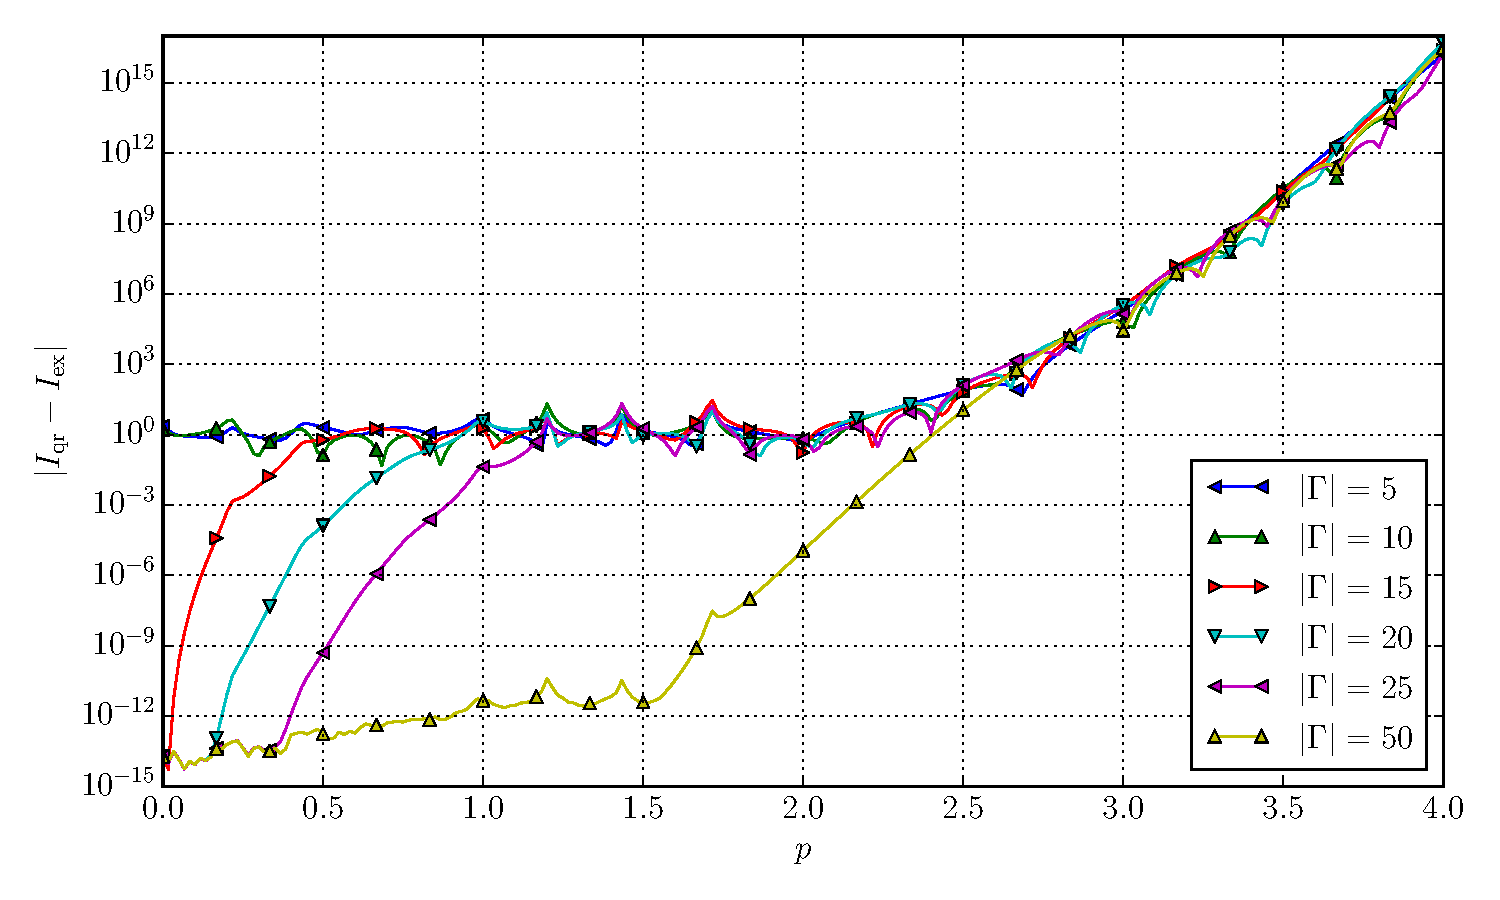
\includegraphics[width=\linewidth]{./plots/tp_1d_conv_p_11_9_err_rel_qr.pdf}
    \caption{Relative error of the direct quadrature method compared to the exact solution.}
    \label{fig:tp_1d_conv_p_11_9_err_rel_qr}
  \end{subfigure}
  \begin{subfigure}[t]{0.5\linewidth}
    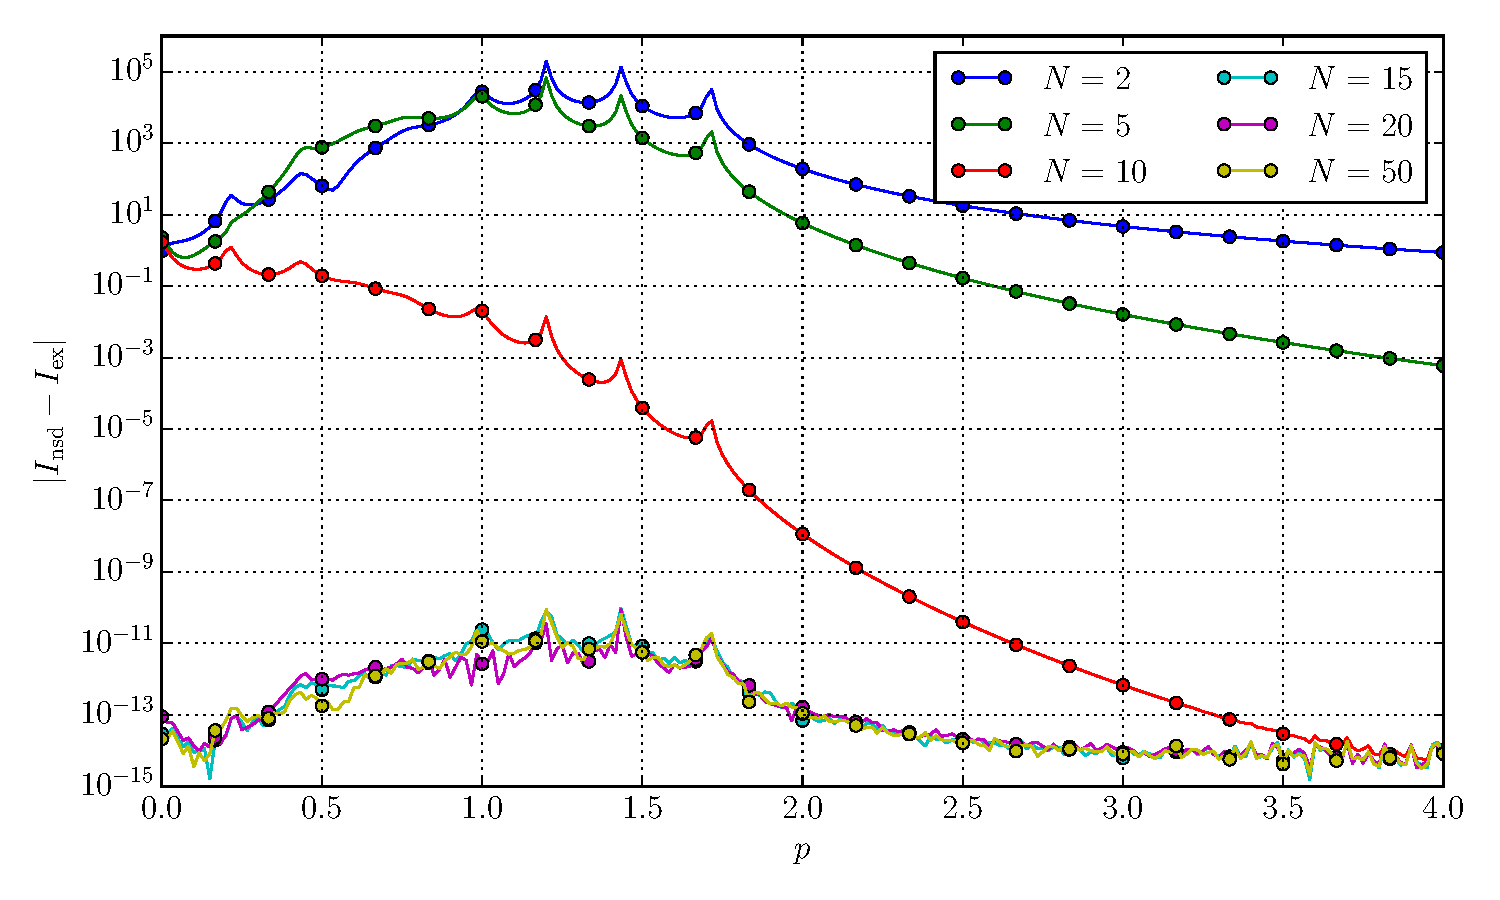
\includegraphics[width=\linewidth]{./plots/tp_1d_conv_p_11_9_err_rel_nsd.pdf}
    \caption{Relative error of the steepest descent method compared to the exact solution.}
    \label{fig:tp_1d_conv_p_11_9_err_rel_nsd}
  \end{subfigure}
  \label{fig:tp_1d_conv_p_11_9}
  \caption{Experiment with $\phi_{11}$ and $\phi_{9}^{\prime}$.
  The parameters are:
  $q=-0.2$, $p=1.2$, $Q=1.0$, $P=1.0\imath$ and
  $q^\prime=0.2$, $p^\prime=-1.2$, $Q^\prime=0.5$, $P^\prime=2.0\imath$
  with $\varepsilon=0.3$.}
\end{figure}

\begin{figure}[ht!]
  \begin{subfigure}[t]{0.5\linewidth}
    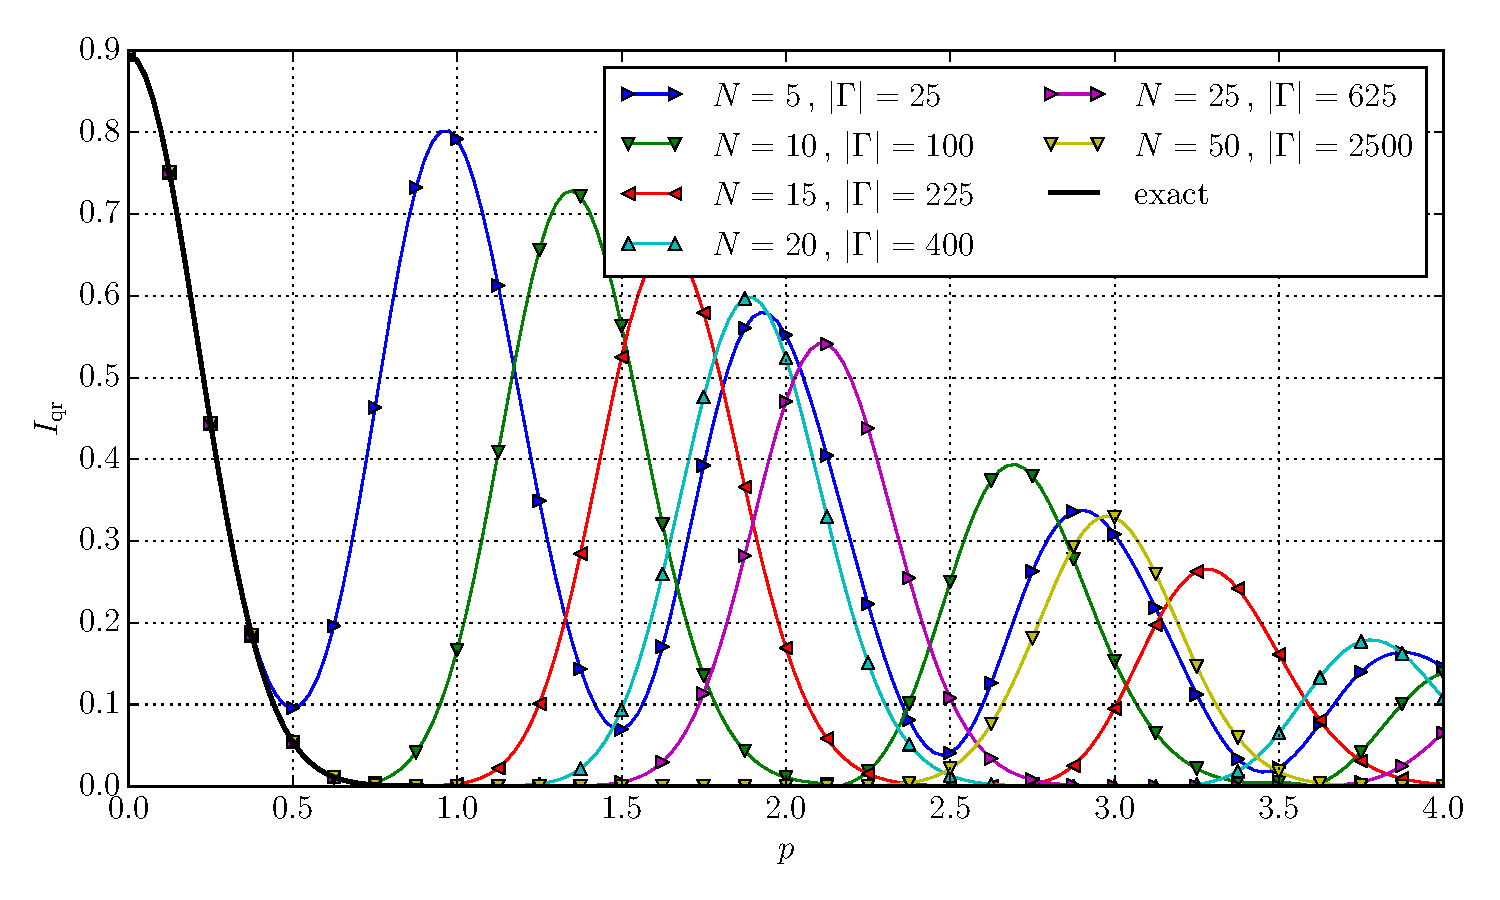
\includegraphics[width=\linewidth]{./plots/tp_2d_conv_p_(0,0)_(0,0)_val_qr.pdf}
    \caption{Direct tensor product Gauss-Hermite quadrature of linear size $N$ with a total of $|\Gamma|$ nodes.}
    \label{fig:tp_2d_conv_p_00_00_val_qr}
  \end{subfigure}
  \begin{subfigure}[t]{0.5\linewidth}
    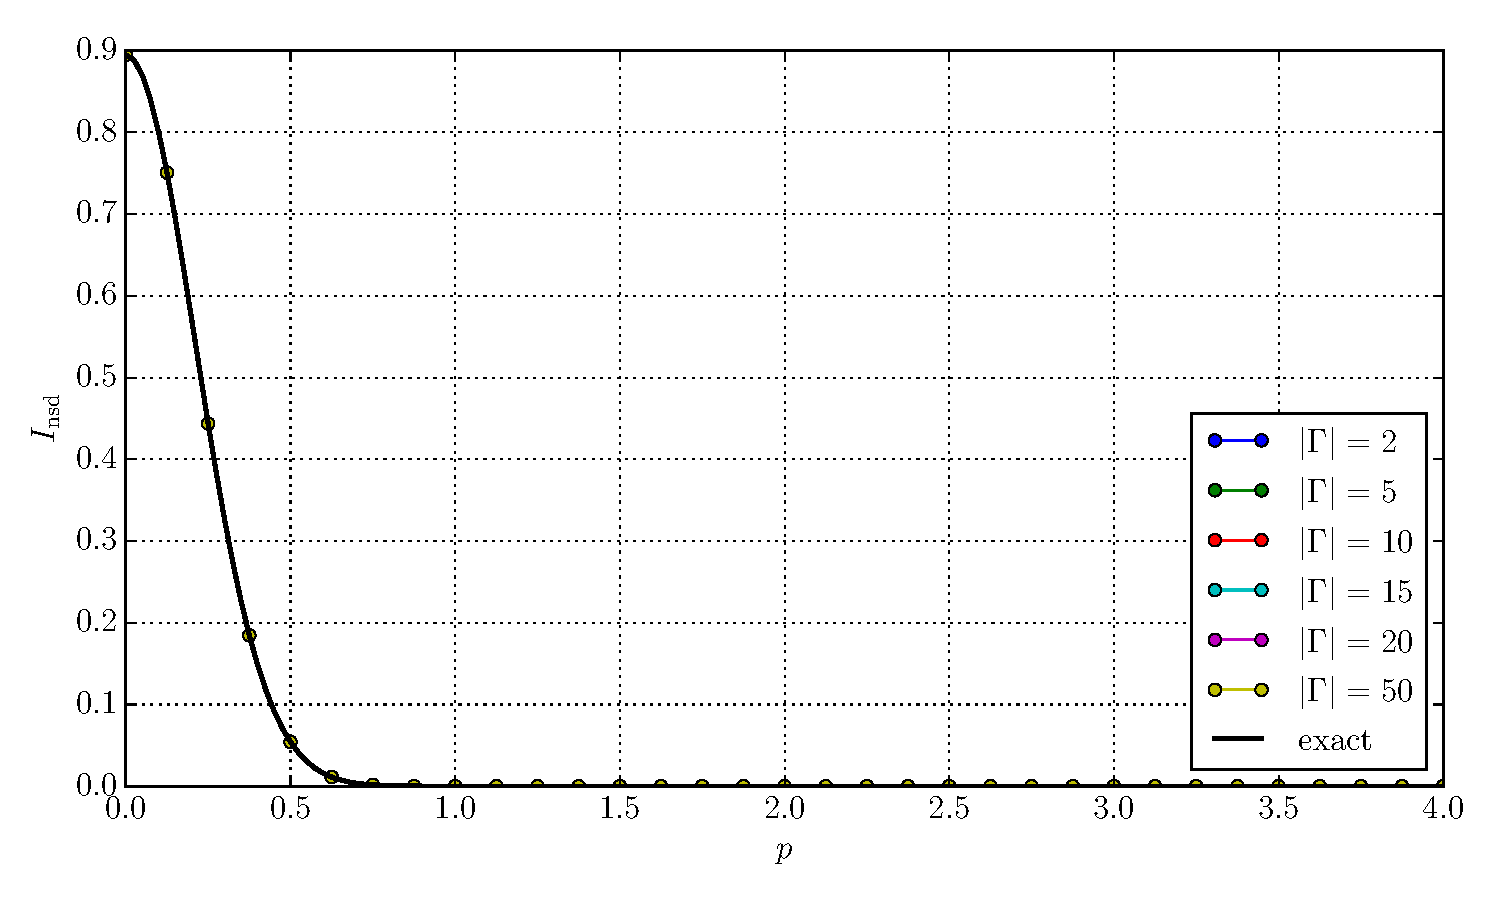
\includegraphics[width=\linewidth]{./plots/tp_2d_conv_p_(0,0)_(0,0)_val_nsd.pdf}
    \caption{Steepest descent transformation and tensor product Gauss-Hermite quadrature of linear size $N$ with a total of $|\Gamma|$ nodes.}
    \label{fig:tp_2d_conv_p_00_00_val_nsd}
  \end{subfigure} \\
  \begin{subfigure}[t]{0.5\linewidth}
    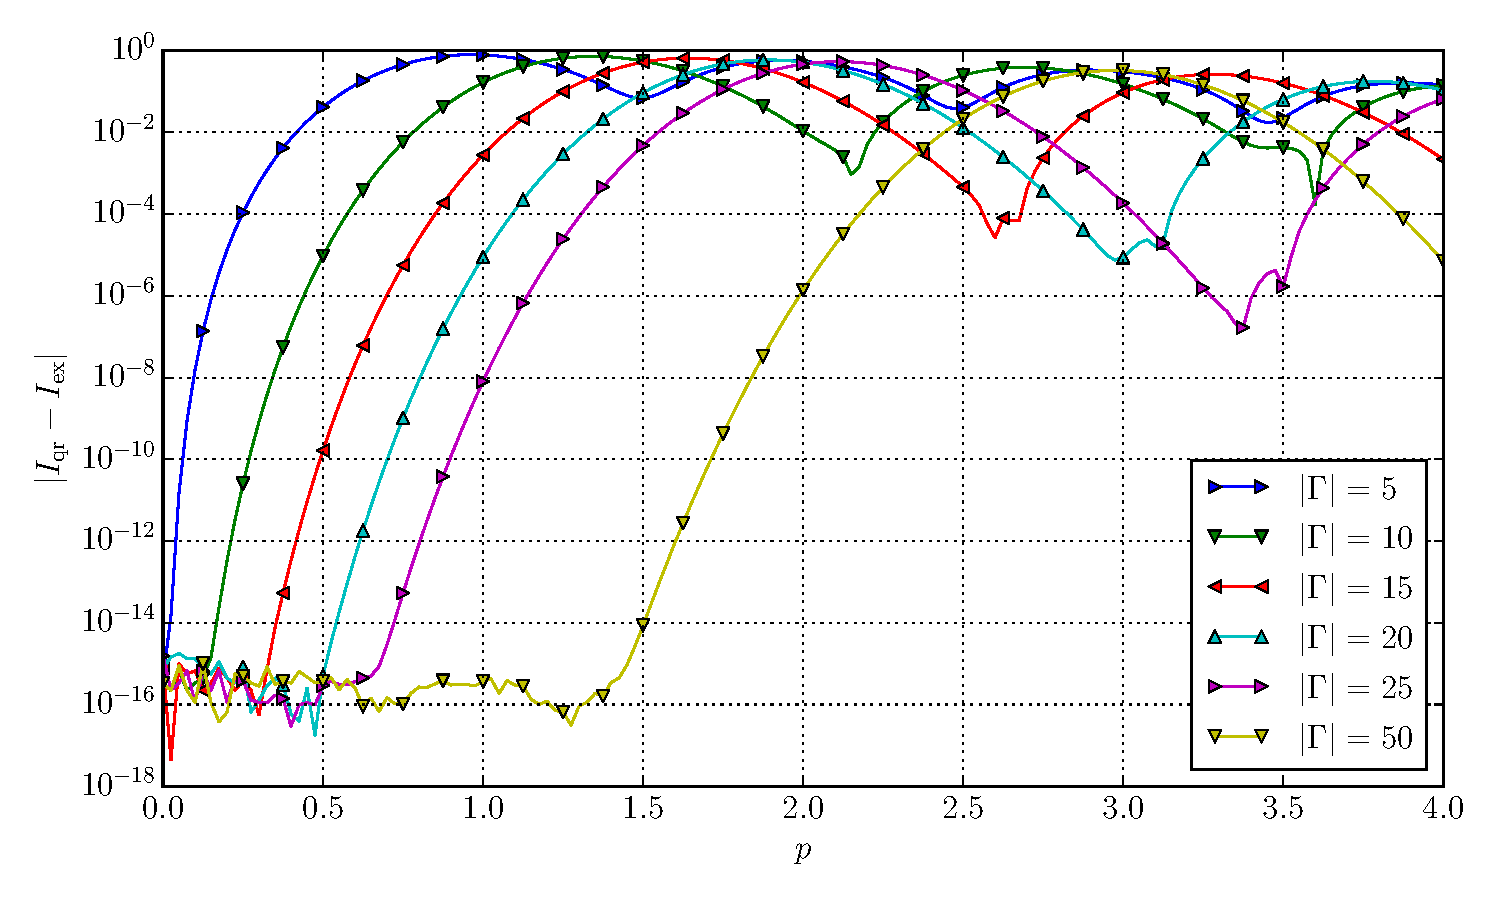
\includegraphics[width=\linewidth]{./plots/tp_2d_conv_p_(0,0)_(0,0)_err_qr.pdf}
    \caption{Absolute error of the direct quadrature method compared to the exact solution.}
    \label{fig:tp_2d_conv_p_00_00_err_qr}
  \end{subfigure}
  \begin{subfigure}[t]{0.5\linewidth}
    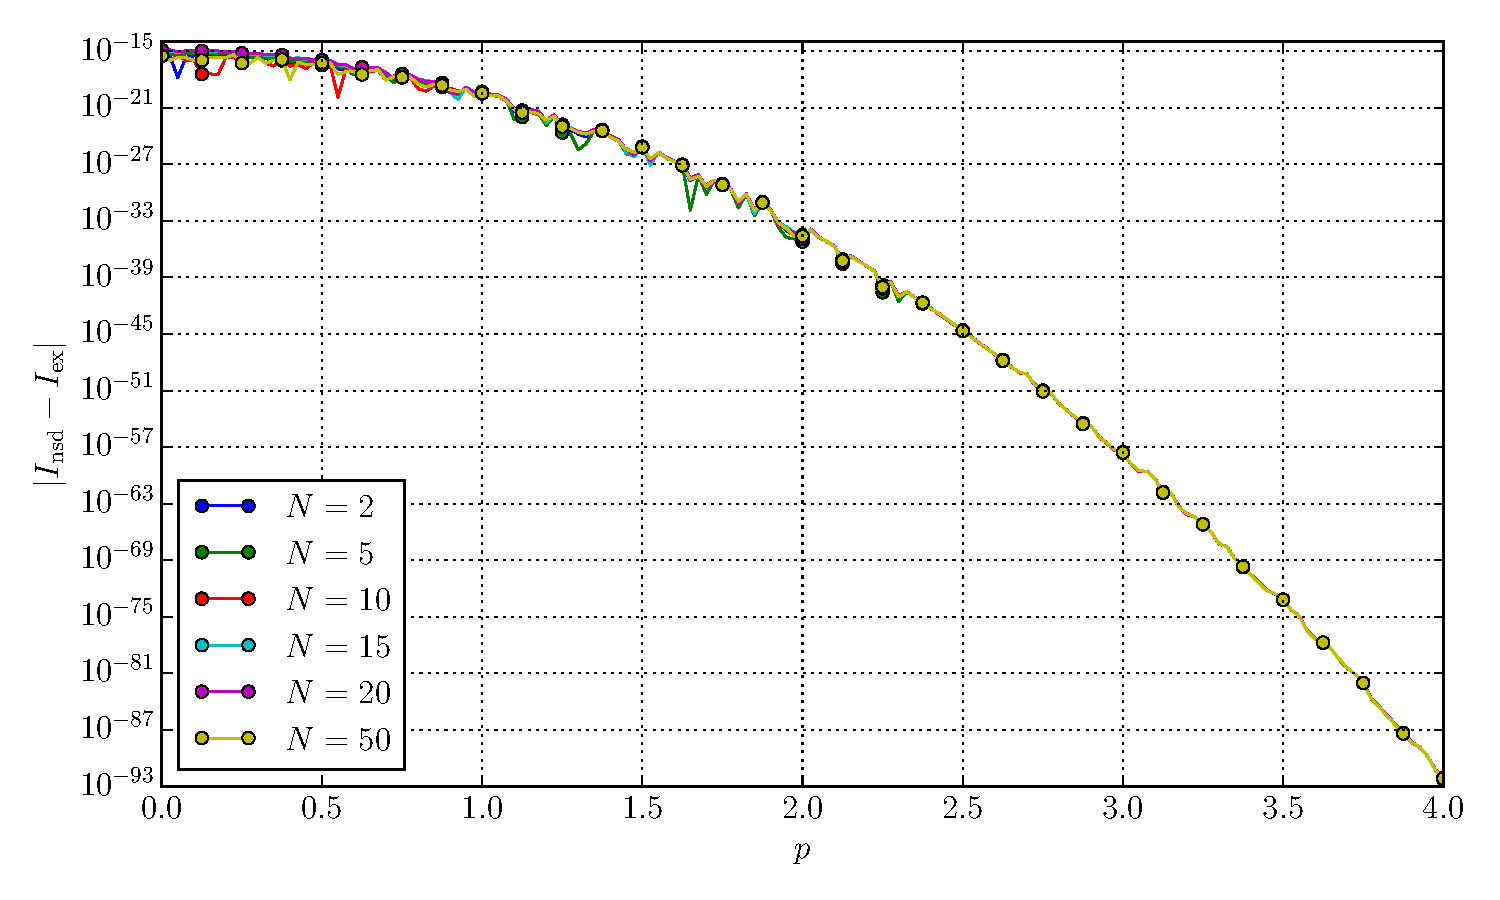
\includegraphics[width=\linewidth]{./plots/tp_2d_conv_p_(0,0)_(0,0)_err_nsd.pdf}
    \caption{Absolute error of the steepest descent method compared to the exact solution.}
    \label{fig:tp_2d_conv_p_00_00_err_nsd}
  \end{subfigure}
  \begin{subfigure}[t]{0.5\linewidth}
    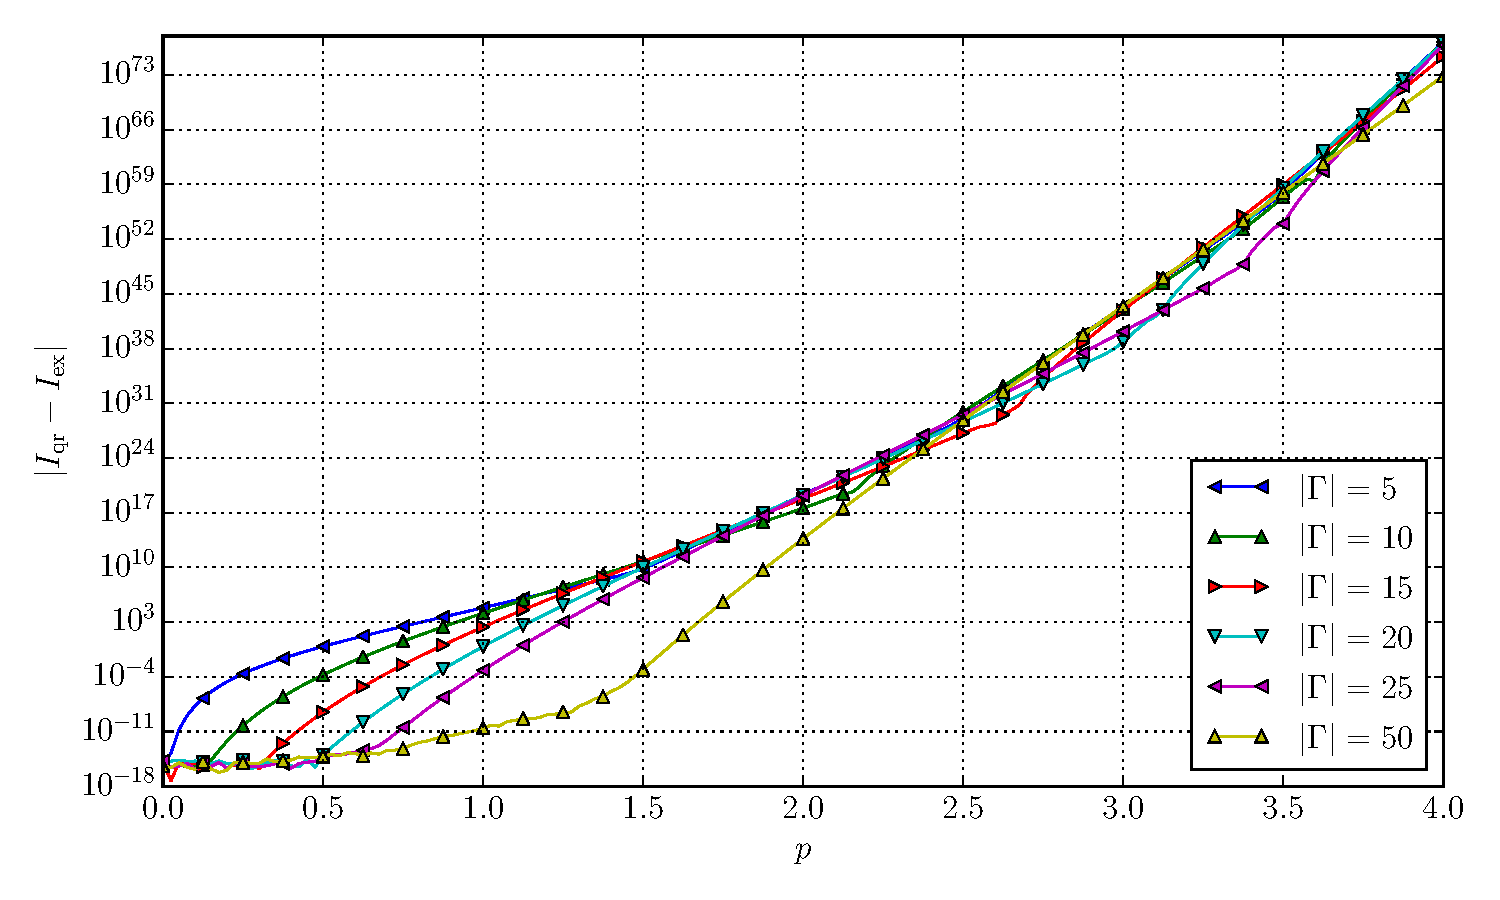
\includegraphics[width=\linewidth]{./plots/tp_2d_conv_p_(0,0)_(0,0)_err_rel_qr.pdf}
    \caption{Relative error of the direct quadrature method compared to the exact solution.}
    \label{fig:tp_2d_conv_p_00_00_err_rel_qr}
  \end{subfigure}
  \begin{subfigure}[t]{0.5\linewidth}
    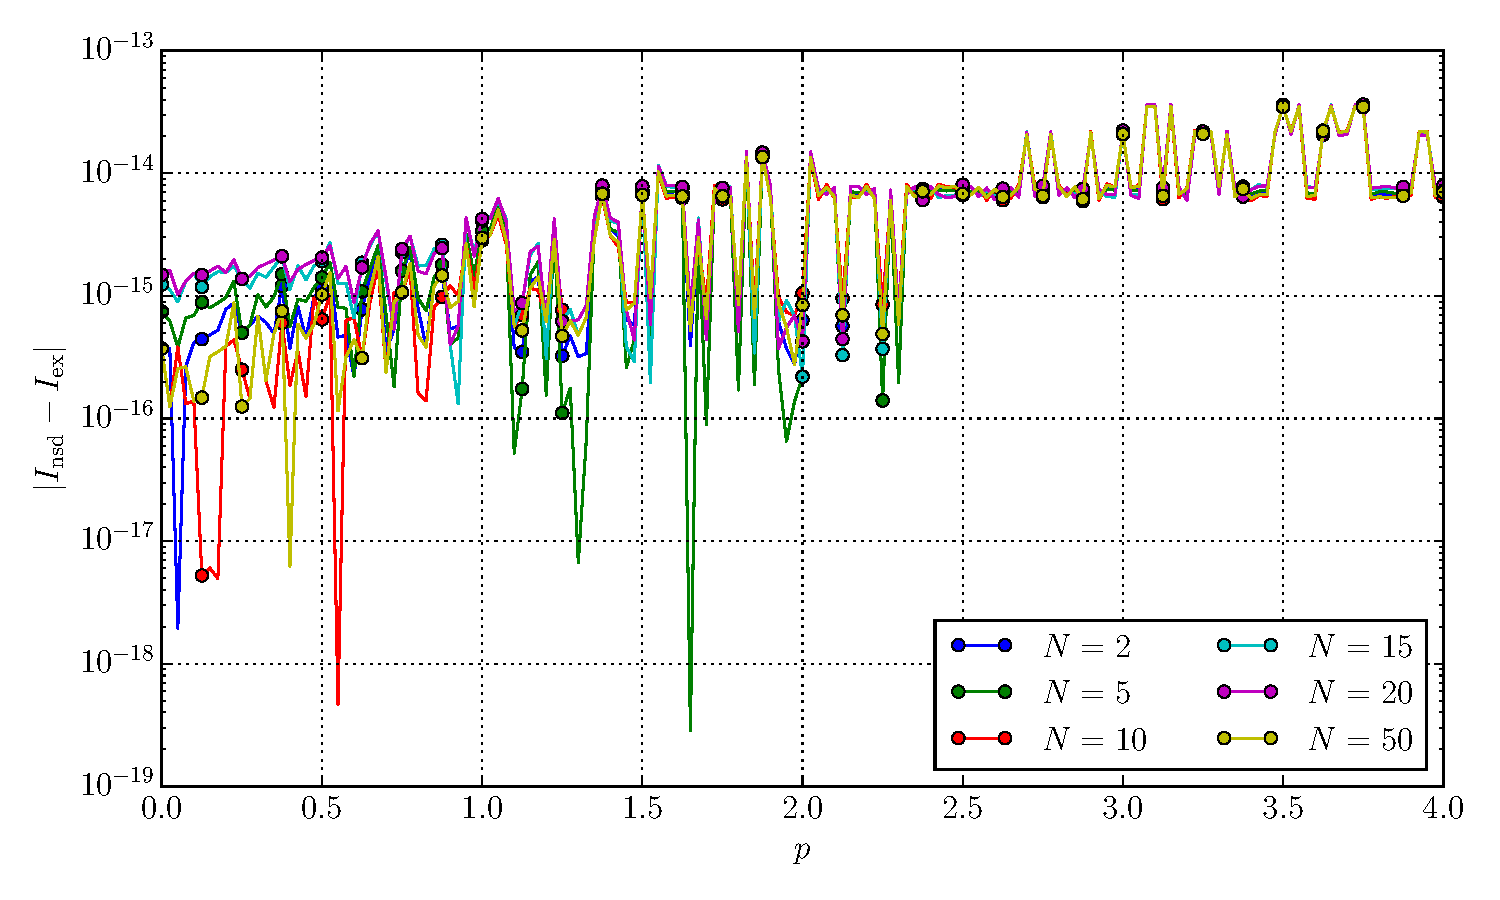
\includegraphics[width=\linewidth]{./plots/tp_2d_conv_p_(0,0)_(0,0)_err_rel_nsd.pdf}
    \caption{Relative error of the steepest descent method compared to the exact solution.}
    \label{fig:tp_2d_conv_p_00_00_err_rel_nsd}
  \end{subfigure}
  \label{fig:tp_2d_conv_p_00_00}
  \caption{Experiment with $\phi_{0,0}$ and $\phi_{0,0}^{\prime}$.
  The parameters are:
  $\vec{q} = (-0.1,  0.1)$,
  $\vec{p} = ( 1.0, -0.1)$,
  $\mat{Q} = \mat{1}$,
  $\mat{P} = \imath \mat{1}$
  and
  $\vec{q}^\prime = ( 0.1, 0.1)$,
  $\vec{p}^\prime = (-1.0, 0.1)$,
  $\mat{Q}^\prime = \mat{1}$,
  $\mat{P}^\prime = \imath \mat{1}$
  with $\varepsilon=0.3$.}
\end{figure}

\begin{figure}[ht!]
  \begin{subfigure}[t]{0.5\linewidth}
    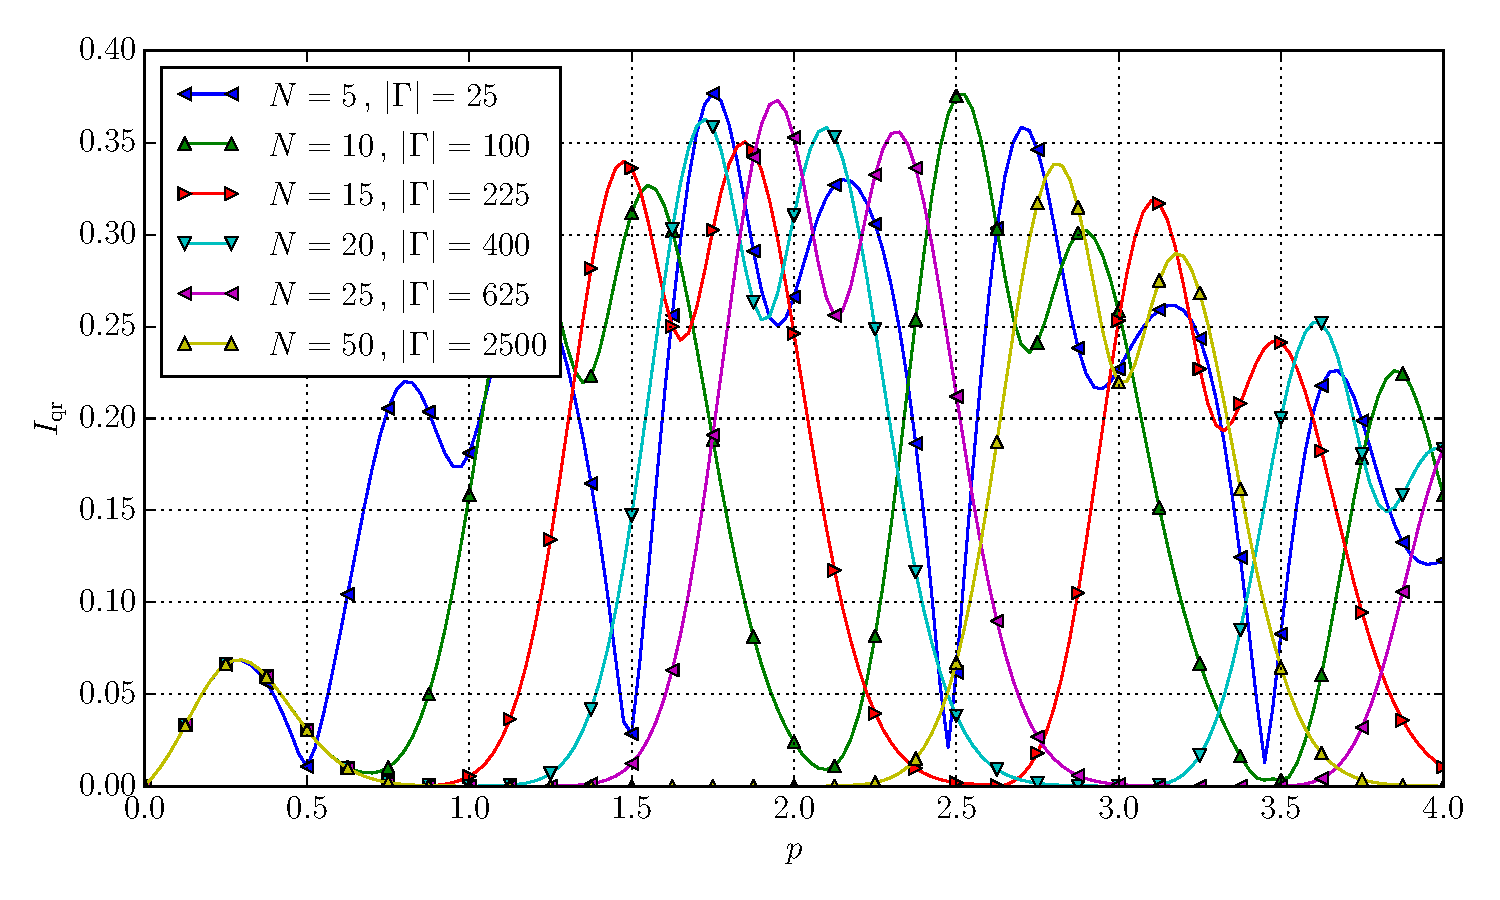
\includegraphics[width=\linewidth]{./plots/tp_2d_conv_p_(1,0)_(0,1)_val_qr.pdf}
    \caption{Direct tensor product Gauss-Hermite quadrature of linear size $N$ with a total of $|\Gamma|$ nodes.}
    \label{fig:tp_2d_conv_p_10_01_val_qr}
  \end{subfigure}
  \begin{subfigure}[t]{0.5\linewidth}
    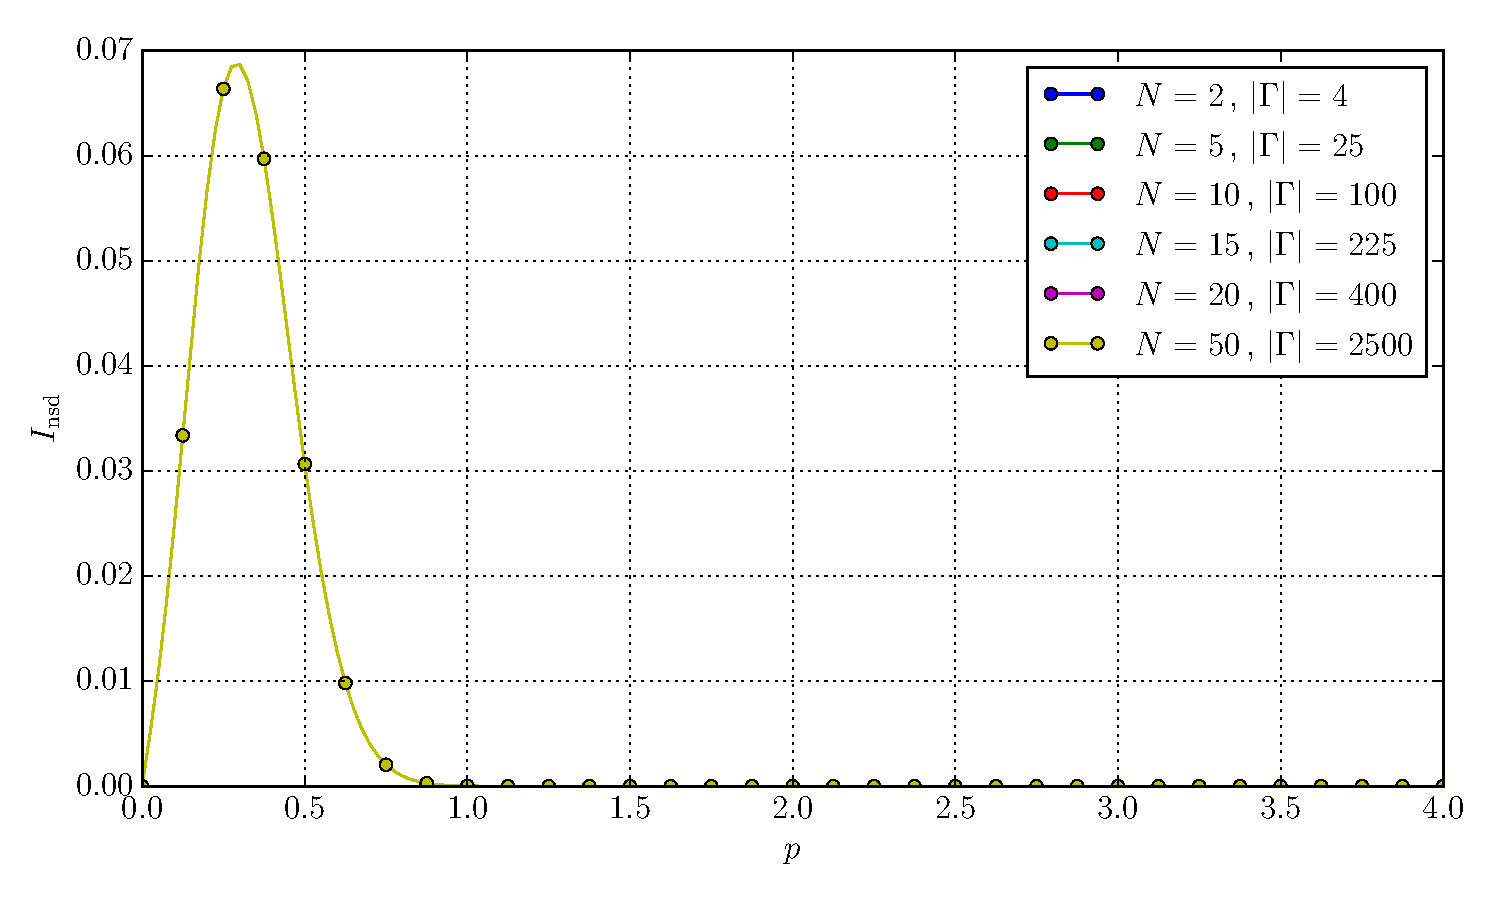
\includegraphics[width=\linewidth]{./plots/tp_2d_conv_p_(1,0)_(0,1)_val_nsd.pdf}
    \caption{Steepest descent transformation and tensor product Gauss-Hermite quadrature of linear size $N$ with a total of $|\Gamma|$ nodes.}
    \label{fig:tp_2d_conv_p_10_01_val_nsd}
  \end{subfigure} \\
  \begin{subfigure}[t]{0.5\linewidth}
    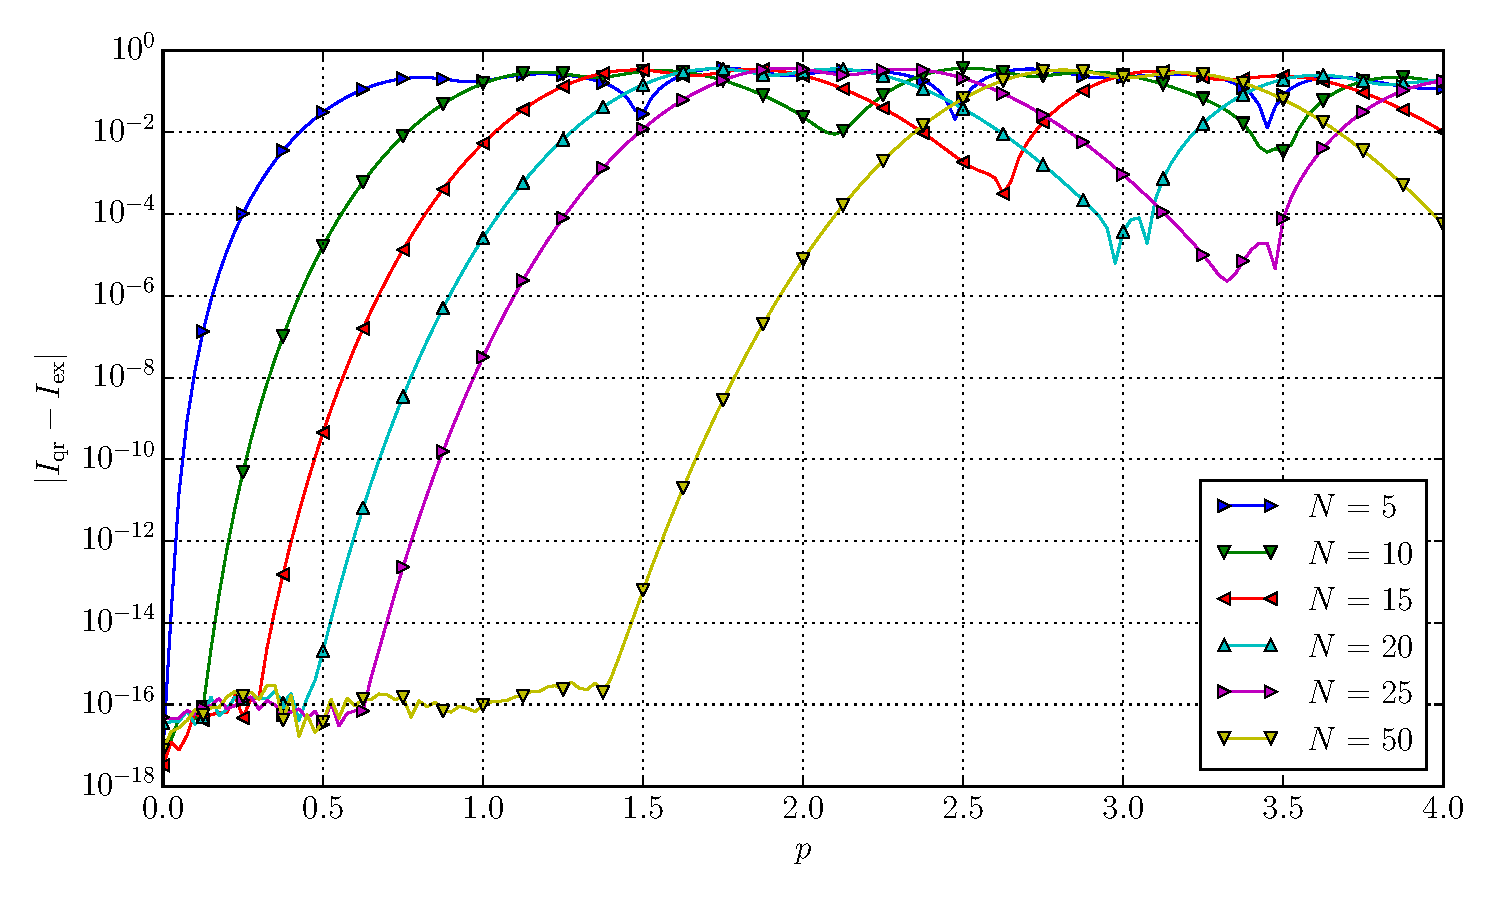
\includegraphics[width=\linewidth]{./plots/tp_2d_conv_p_(1,0)_(0,1)_err_qr.pdf}
    \caption{Absolute error of the direct quadrature method compared to the exact solution.}
    \label{fig:tp_2d_conv_p_10_01_err_qr}
  \end{subfigure}
  \begin{subfigure}[t]{0.5\linewidth}
    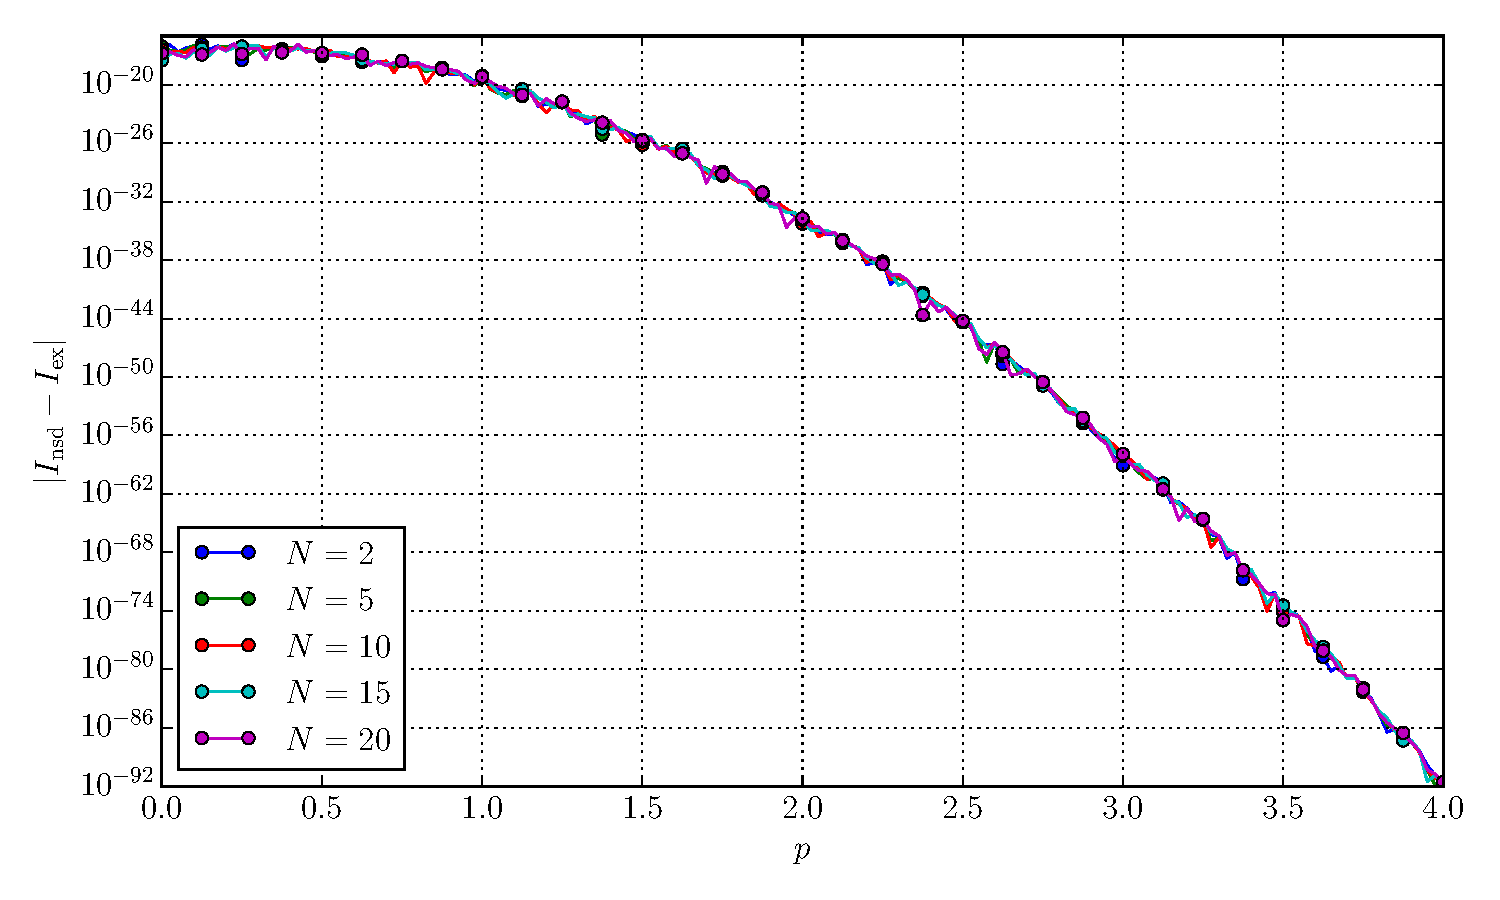
\includegraphics[width=\linewidth]{./plots/tp_2d_conv_p_(1,0)_(0,1)_err_nsd.pdf}
    \caption{Absolute error of the steepest descent method compared to the exact solution.}
    \label{fig:tp_2d_conv_p_10_01_err_nsd}
  \end{subfigure}
  \begin{subfigure}[t]{0.5\linewidth}
    \includegraphics[width=\linewidth]{./plots/tp_2d_conv_p_(1,0)_(0,1)_err_rel_qr.pdf}
    \caption{Relative error of the direct quadrature method compared to the exact solution.}
    \label{fig:tp_2d_conv_p_10_01_err_rel_qr}
  \end{subfigure}
  \begin{subfigure}[t]{0.5\linewidth}
    \includegraphics[width=\linewidth]{./plots/tp_2d_conv_p_(1,0)_(0,1)_err_rel_nsd.pdf}
    \caption{Relative error of the steepest descent method compared to the exact solution.}
    \label{fig:tp_2d_conv_p_10_01_err_rel_nsd}
  \end{subfigure}
  \label{fig:tp_2d_conv_p_10_01}
  \caption{Experiment with $\phi_{1,0}$ and $\phi_{0,1}^{\prime}$.
  The parameters are:
  $\vec{q} = (-0.1,  0.1)$,
  $\vec{p} = ( 1.0, -0.1)$,
  $\mat{Q} = \mat{1}$,
  $\mat{P} = \imath \mat{1}$
  and
  $\vec{q}^\prime = ( 0.1, 0.1)$,
  $\vec{p}^\prime = (-1.0, 0.1)$,
  $\mat{Q}^\prime = \mat{1}$,
  $\mat{P}^\prime = \imath \mat{1}$
  with $\varepsilon=0.3$.}
\end{figure}

\begin{figure}[ht!]
  \begin{subfigure}[t]{0.5\linewidth}
    \includegraphics[width=\linewidth]{./plots/tp_2d_conv_p_(8,8)_(8,8)_val_qr.pdf}
    \caption{Direct tensor product Gauss-Hermite quadrature of linear size $N$ with a total of $|\Gamma|$ nodes.}
    \label{fig:tp_2d_conv_p_88_88_val_qr}
  \end{subfigure}
  \begin{subfigure}[t]{0.5\linewidth}
    \includegraphics[width=\linewidth]{./plots/tp_2d_conv_p_(8,8)_(8,8)_val_nsd.pdf}
    \caption{Steepest descent transformation and tensor product Gauss-Hermite quadrature of linear size $N$ with a total of $|\Gamma|$ nodes.}
    \label{fig:tp_2d_conv_p_88_88_val_nsd}
  \end{subfigure} \\
  \begin{subfigure}[t]{0.5\linewidth}
    \includegraphics[width=\linewidth]{./plots/tp_2d_conv_p_(8,8)_(8,8)_err_qr.pdf}
    \caption{Absolute error of the direct quadrature method compared to the exact solution.}
    \label{fig:tp_2d_conv_p_88_88_err_qr}
  \end{subfigure}
  \begin{subfigure}[t]{0.5\linewidth}
    \includegraphics[width=\linewidth]{./plots/tp_2d_conv_p_(8,8)_(8,8)_err_nsd.pdf}
    \caption{Absolute error of the steepest descent method compared to the exact solution.}
    \label{fig:tp_2d_conv_p_88_88_err_nsd}
  \end{subfigure}
  \begin{subfigure}[t]{0.5\linewidth}
    \includegraphics[width=\linewidth]{./plots/tp_2d_conv_p_(8,8)_(8,8)_err_rel_qr.pdf}
    \caption{Relative error of the direct quadrature method compared to the exact solution.}
    \label{fig:tp_2d_conv_p_88_88_err_rel_qr}
  \end{subfigure}
  \begin{subfigure}[t]{0.5\linewidth}
    \includegraphics[width=\linewidth]{./plots/tp_2d_conv_p_(8,8)_(8,8)_err_rel_nsd.pdf}
    \caption{Relative error of the steepest descent method compared to the exact solution.}
    \label{fig:tp_2d_conv_p_88_88_err_rel_nsd}
  \end{subfigure}
  \label{fig:tp_2d_conv_p_88_88}
  \caption{Experiment with $\phi_{8,8}$ and $\phi_{8,8}^{\prime}$.
  The parameters are:
  $\vec{q} = (-0.1,  0.1)$,
  $\vec{p} = ( 1.0, -0.1)$,
  $\mat{Q} = ( 1.0,       0; 0, 1.0)$,
  $\mat{P} = ( 1.0\imath, 0; 0, 1.0\imath)$
  and
  $\vec{q}^\prime = ( 0.1, 0.1)$,
  $\vec{p}^\prime = (-1.0, 0.1)$,
  $\mat{Q}^\prime = ( 2.0,       0; 0, 0.5)$,
  $\mat{P}^\prime = ( 0.5\imath, 0; 0, 2.0\imath)$
  with $\varepsilon=0.3$.}
\end{figure}

\begin{figure}[ht!]
  \begin{subfigure}[t]{0.5\linewidth}
    \includegraphics[width=\linewidth]{./plots/tp_4d_conv_p_(0,0,0,0)_(0,0,0,0)_val_qr.pdf}
    \caption{Direct tensor product Gauss-Hermite quadrature of linear size $N$ with a total of $|\Gamma|$ nodes.}
    \label{fig:tp_4d_conv_p_0000_0000_val_qr}
  \end{subfigure}
  \begin{subfigure}[t]{0.5\linewidth}
    \includegraphics[width=\linewidth]{./plots/tp_4d_conv_p_(0,0,0,0)_(0,0,0,0)_val_nsd.pdf}
    \caption{Steepest descent transformation and tensor product Gauss-Hermite quadrature of linear size $N$ with a total of $|\Gamma|$ nodes.}
    \label{fig:tp_4d_conv_p_0000_0000_val_nsd}
  \end{subfigure} \\
  \begin{subfigure}[t]{0.5\linewidth}
    \includegraphics[width=\linewidth]{./plots/tp_4d_conv_p_(0,0,0,0)_(0,0,0,0)_err_qr.pdf}
    \caption{Absolute error of the direct quadrature method compared to the exact solution.}
    \label{fig:tp_4d_conv_p_0000_0000_err_qr}
  \end{subfigure}
  \begin{subfigure}[t]{0.5\linewidth}
    \includegraphics[width=\linewidth]{./plots/tp_4d_conv_p_(0,0,0,0)_(0,0,0,0)_err_nsd.pdf}
    \caption{Absolute error of the steepest descent method compared to the exact solution.}
    \label{fig:tp_4d_conv_p_0000_0000_err_nsd}
  \end{subfigure}
  \begin{subfigure}[t]{0.5\linewidth}
    \includegraphics[width=\linewidth]{./plots/tp_4d_conv_p_(0,0,0,0)_(0,0,0,0)_err_rel_qr.pdf}
    \caption{Relative error of the direct quadrature method compared to the exact solution.}
    \label{fig:tp_4d_conv_p_0000_0000_err_rel_qr}
  \end{subfigure}
  \begin{subfigure}[t]{0.5\linewidth}
    \includegraphics[width=\linewidth]{./plots/tp_4d_conv_p_(0,0,0,0)_(0,0,0,0)_err_rel_nsd.pdf}
    \caption{Relative error of the steepest descent method compared to the exact solution.}
    \label{fig:tp_4d_conv_p_0000_0000_err_rel_nsd}
  \end{subfigure}
  \label{fig:tp_4d_conv_p_0000_0000}
  \caption{Experiment with $\phi_{0,0,0,0}$ and $\phi_{0,0,0,0}^{\prime}$.
  The parameters are:
  $\vec{q} = (-0.1, -0.1, -0.1, -0.1)$,
  $\vec{p} = ( 0.2, -0.2, -0.2,  0.2)$,
  $\mat{Q} = \mat{1}$,
  $\mat{P} = \imath \mat{1}$
  and
  $\vec{q}^\prime = ( 0.1, 0.1, 0.1,  0.1)$,
  $\vec{p}^\prime = (-0.2, 0.2, 0.2, -0.2)$,
  $\mat{Q}^\prime = \mat{1}$,
  $\mat{P}^\prime = \imath \mat{1}$
  with $\varepsilon=0.1$.}
\end{figure}

\begin{figure}[ht!]
  \begin{subfigure}[t]{0.5\linewidth}
    \includegraphics[width=\linewidth]{./plots/tp_4d_conv_p_(1,1,1,1)_(1,1,1,1)_val_qr.pdf}
    \caption{Direct tensor product Gauss-Hermite quadrature of linear size $N$ with a total of $|\Gamma|$ nodes.}
    \label{fig:tp_4d_conv_p_1111_1111_val_qr}
  \end{subfigure}
  \begin{subfigure}[t]{0.5\linewidth}
    \includegraphics[width=\linewidth]{./plots/tp_4d_conv_p_(1,1,1,1)_(1,1,1,1)_val_nsd.pdf}
    \caption{Steepest descent transformation and tensor product Gauss-Hermite quadrature of linear size $N$ with a total of $|\Gamma|$ nodes.}
    \label{fig:tp_4d_conv_p_1111_1111_val_nsd}
  \end{subfigure} \\
  \begin{subfigure}[t]{0.5\linewidth}
    \includegraphics[width=\linewidth]{./plots/tp_4d_conv_p_(1,1,1,1)_(1,1,1,1)_err_qr.pdf}
    \caption{Absolute error of the direct quadrature method compared to the exact solution.}
    \label{fig:tp_4d_conv_p_1111_1111_err_qr}
  \end{subfigure}
  \begin{subfigure}[t]{0.5\linewidth}
    \includegraphics[width=\linewidth]{./plots/tp_4d_conv_p_(1,1,1,1)_(1,1,1,1)_err_nsd.pdf}
    \caption{Absolute error of the steepest descent method compared to the exact solution.}
    \label{fig:tp_4d_conv_p_1111_1111_err_nsd}
  \end{subfigure}
  \begin{subfigure}[t]{0.5\linewidth}
    \includegraphics[width=\linewidth]{./plots/tp_4d_conv_p_(1,1,1,1)_(1,1,1,1)_err_rel_qr.pdf}
    \caption{Relative error of the direct quadrature method compared to the exact solution.}
    \label{fig:tp_4d_conv_p_1111_1111_err_rel_qr}
  \end{subfigure}
  \begin{subfigure}[t]{0.5\linewidth}
    \includegraphics[width=\linewidth]{./plots/tp_4d_conv_p_(1,1,1,1)_(1,1,1,1)_err_rel_nsd.pdf}
    \caption{Relative error of the steepest descent method compared to the exact solution.}
    \label{fig:tp_4d_conv_p_1111_1111_err_rel_nsd}
  \end{subfigure}
  \label{fig:tp_4d_conv_p_1111_1111}
  \caption{Experiment with $\phi_{1,1,1,1}$ and $\phi_{1,1,1,1}^{\prime}$.
  The parameters are:
  $\vec{q} = (-0.1, -0.1, -0.1, -0.1)$,
  $\vec{p} = ( 0.2, -0.2, -0.2,  0.2)$,
  $\mat{Q} = \mat{1}$,
  $\mat{P} = \imath \mat{1}$
  and
  $\vec{q}^\prime = ( 0.1, 0.1, 0.1,  0.1)$,
  $\vec{p}^\prime = (-0.2, 0.2, 0.2, -0.2)$,
  $\mat{Q}^\prime = \mat{1}$,
  $\mat{P}^\prime = \imath \mat{1}$
  with $\varepsilon=0.1$.}
\end{figure}


\FloatBarrier
\subsubsection{Convergence in $\varepsilon$}


\begin{figure}[ht!]
  \begin{subfigure}[t]{0.5\linewidth}
    \includegraphics[width=\linewidth]{./plots/tp_1d_conv_eps_0_0_val_qr.pdf}
    \caption{Direct Gauss-Hermite quadrature of size $N$ with a total of $|\Gamma|$ nodes.}
    \label{fig:tp_1d_conv_eps_0_0_val_qr}
  \end{subfigure}
  \begin{subfigure}[t]{0.5\linewidth}
    \includegraphics[width=\linewidth]{./plots/tp_1d_conv_eps_0_0_val_nsd.pdf}
    \caption{Steepest descent transformation and Gauss-Hermite quadrature of size $N$ with a total of $|\Gamma|$ nodes.}
    \label{fig:tp_1d_conv_eps_0_0_val_nsd}
  \end{subfigure} \\
  \begin{subfigure}[t]{0.5\linewidth}
    \includegraphics[width=\linewidth]{./plots/tp_1d_conv_eps_0_0_err_qr.pdf}
    \caption{Absolute error of the direct quadrature method compared to the exact solution.}
    \label{fig:tp_1d_conv_eps_0_0_err_qr}
  \end{subfigure}
  \begin{subfigure}[t]{0.5\linewidth}
    \includegraphics[width=\linewidth]{./plots/tp_1d_conv_eps_0_0_err_nsd.pdf}
    \caption{Absolute error of the steepest descent method compared to the exact solution.}
    \label{fig:tp_1d_conv_eps_0_0_err_nsd}
  \end{subfigure}
  \begin{subfigure}[t]{0.5\linewidth}
    \includegraphics[width=\linewidth]{./plots/tp_1d_conv_eps_0_0_err_rel_qr.pdf}
    \caption{Relative error of the direct quadrature method compared to the exact solution.}
    \label{fig:tp_1d_conv_eps_0_0_err_rel_qr}
  \end{subfigure}
  \begin{subfigure}[t]{0.5\linewidth}
    \includegraphics[width=\linewidth]{./plots/tp_1d_conv_eps_0_0_err_rel_nsd.pdf}
    \caption{Relative error of the steepest descent method compared to the exact solution.}
    \label{fig:tp_1d_conv_eps_0_0_err_rel_nsd}
  \end{subfigure}
  \label{fig:tp_1d_conv_eps_0_0}
  \caption{Experiment with $\phi_{0}$ and $\phi_{0}^{\prime}$.
  The parameters are:
  $q=1.0$, $p=0.2$, $Q=0.5$, $P=2.0\imath$ and
  $q^\prime=1.0$, $p^\prime=-0.2$, $Q^\prime=2.0$, $P^\prime=0.5\imath$.}
\end{figure}

\begin{figure}[ht!]
  \begin{subfigure}[t]{0.5\linewidth}
    \includegraphics[width=\linewidth]{./plots/tp_1d_conv_eps_2_1_val_qr.pdf}
    \caption{Direct Gauss-Hermite quadrature of size $N$ with a total of $|\Gamma|$ nodes.}
    \label{fig:tp_1d_conv_eps_2_1_val_qr}
  \end{subfigure}
  \begin{subfigure}[t]{0.5\linewidth}
    \includegraphics[width=\linewidth]{./plots/tp_1d_conv_eps_2_1_val_nsd.pdf}
    \caption{Steepest descent transformation and Gauss-Hermite quadrature of size $N$ with a total of $|\Gamma|$ nodes.}
    \label{fig:tp_1d_conv_eps_2_1_val_nsd}
  \end{subfigure} \\
  \begin{subfigure}[t]{0.5\linewidth}
    \includegraphics[width=\linewidth]{./plots/tp_1d_conv_eps_2_1_err_qr.pdf}
    \caption{Absolute error of the direct quadrature method compared to the exact solution.}
    \label{fig:tp_1d_conv_eps_2_1_err_qr}
  \end{subfigure}
  \begin{subfigure}[t]{0.5\linewidth}
    \includegraphics[width=\linewidth]{./plots/tp_1d_conv_eps_2_1_err_nsd.pdf}
    \caption{Absolute error of the steepest descent method compared to the exact solution.}
    \label{fig:tp_1d_conv_eps_2_1_err_nsd}
  \end{subfigure}
  \begin{subfigure}[t]{0.5\linewidth}
    \includegraphics[width=\linewidth]{./plots/tp_1d_conv_eps_2_1_err_rel_qr.pdf}
    \caption{Relative error of the direct quadrature method compared to the exact solution.}
    \label{fig:tp_1d_conv_eps_2_1_err_rel_qr}
  \end{subfigure}
  \begin{subfigure}[t]{0.5\linewidth}
    \includegraphics[width=\linewidth]{./plots/tp_1d_conv_eps_2_1_err_rel_nsd.pdf}
    \caption{Relative error of the steepest descent method compared to the exact solution.}
    \label{fig:tp_1d_conv_eps_2_1_err_rel_nsd}
  \end{subfigure}
  \label{fig:tp_1d_conv_eps_2_1}
  \caption{Experiment with $\phi_{2}$ and $\phi_{1}^{\prime}$.
  The parameters are:
  $q=1.0$, $p=0.2$, $Q=0.5$, $P=2.0\imath$ and
  $q^\prime=1.0$, $p^\prime=-0.2$, $Q^\prime=2.0$, $P^\prime=0.5\imath$.}
\end{figure}

\begin{figure}[ht!]
  \begin{subfigure}[t]{0.5\linewidth}
    \includegraphics[width=\linewidth]{./plots/tp_1d_conv_eps_8_8_val_qr.pdf}
    \caption{Direct Gauss-Hermite quadrature of size $N$ with a total of $|\Gamma|$ nodes.}
    \label{fig:tp_1d_conv_eps_8_8_val_qr}
  \end{subfigure}
  \begin{subfigure}[t]{0.5\linewidth}
    \includegraphics[width=\linewidth]{./plots/tp_1d_conv_eps_8_8_val_nsd.pdf}
    \caption{Steepest descent transformation and Gauss-Hermite quadrature of size $N$ with a total of $|\Gamma|$ nodes.}
    \label{fig:tp_1d_conv_eps_8_8_val_nsd}
  \end{subfigure} \\
  \begin{subfigure}[t]{0.5\linewidth}
    \includegraphics[width=\linewidth]{./plots/tp_1d_conv_eps_8_8_err_qr.pdf}
    \caption{Absolute error of the direct quadrature method compared to the exact solution.}
    \label{fig:tp_1d_conv_eps_8_8_err_qr}
  \end{subfigure}
  \begin{subfigure}[t]{0.5\linewidth}
    \includegraphics[width=\linewidth]{./plots/tp_1d_conv_eps_8_8_err_nsd.pdf}
    \caption{Absolute error of the steepest descent method compared to the exact solution.}
    \label{fig:tp_1d_conv_eps_8_8_err_nsd}
  \end{subfigure}
  \begin{subfigure}[t]{0.5\linewidth}
    \includegraphics[width=\linewidth]{./plots/tp_1d_conv_eps_8_8_err_rel_qr.pdf}
    \caption{Relative error of the direct quadrature method compared to the exact solution.}
    \label{fig:tp_1d_conv_eps_8_8_err_rel_qr}
  \end{subfigure}
  \begin{subfigure}[t]{0.5\linewidth}
    \includegraphics[width=\linewidth]{./plots/tp_1d_conv_eps_8_8_err_rel_nsd.pdf}
    \caption{Relative error of the steepest descent method compared to the exact solution.}
    \label{fig:tp_1d_conv_eps_8_8_err_rel_nsd}
  \end{subfigure}
  \label{fig:tp_1d_conv_eps_8_8}
  \caption{Experiment with $\phi_{8}$ and $\phi_{8}^{\prime}$.
  The parameters are:
  $q=1.0$, $p=0.2$, $Q=0.5$, $P=2.0\imath$ and
  $q^\prime=1.0$, $p^\prime=-0.2$, $Q^\prime=2.0$, $P^\prime=0.5\imath$.}
\end{figure}

\begin{figure}[ht!]
  \begin{subfigure}[t]{0.5\linewidth}
    \includegraphics[width=\linewidth]{./plots/tp_2d_conv_eps_(0,0)_(0,0)_val_qr.pdf}
    \caption{Direct tensor product Gauss-Hermite quadrature of linear size $N$ with a total of $|\Gamma|$ nodes.}
    \label{fig:tp_2d_conv_eps_00_00_val_qr}
  \end{subfigure}
  \begin{subfigure}[t]{0.5\linewidth}
    \includegraphics[width=\linewidth]{./plots/tp_2d_conv_eps_(0,0)_(0,0)_val_nsd.pdf}
    \caption{Steepest descent transformation and tensor product Gauss-Hermite quadrature of linear size $N$ with a total of $|\Gamma|$ nodes.}
    \label{fig:tp_2d_conv_eps_00_00_val_nsd}
  \end{subfigure} \\
  \begin{subfigure}[t]{0.5\linewidth}
    \includegraphics[width=\linewidth]{./plots/tp_2d_conv_eps_(0,0)_(0,0)_err_qr.pdf}
    \caption{Absolute error of the direct quadrature method compared to the exact solution.}
    \label{fig:tp_2d_conv_eps_00_00_err_qr}
  \end{subfigure}
  \begin{subfigure}[t]{0.5\linewidth}
    \includegraphics[width=\linewidth]{./plots/tp_2d_conv_eps_(0,0)_(0,0)_err_nsd.pdf}
    \caption{Absolute error of the steepest descent method compared to the exact solution.}
    \label{fig:tp_2d_conv_eps_00_00_err_nsd}
  \end{subfigure}
  \begin{subfigure}[t]{0.5\linewidth}
    \includegraphics[width=\linewidth]{./plots/tp_2d_conv_eps_(0,0)_(0,0)_err_rel_qr.pdf}
    \caption{Relative error of the direct quadrature method compared to the exact solution.}
    \label{fig:tp_2d_conv_eps_00_00_err_rel_qr}
  \end{subfigure}
  \begin{subfigure}[t]{0.5\linewidth}
    \includegraphics[width=\linewidth]{./plots/tp_2d_conv_eps_(0,0)_(0,0)_err_rel_nsd.pdf}
    \caption{Relative error of the steepest descent method compared to the exact solution.}
    \label{fig:tp_2d_conv_eps_00_00_err_rel_nsd}
  \end{subfigure}
  \label{fig:tp_2d_conv_eps_00_00}
  \caption{Experiment with $\phi_{0,0}$ and $\phi_{0,0}^{\prime}$.
  The parameters are:
  $\vec{q} = (1, 1)$,
  $\vec{p} = (-0.2, -0.2)$,
  $\mat{Q} = \mat{1}$,
  $\mat{P} = \imath \mat{1}$
  and
  $\vec{q}^\prime = (1, 1)$,
  $\vec{p}^\prime = (0.2, 0.2)$,
  $\mat{Q}^\prime = \mat{1}$,
  $\mat{P}^\prime = \imath \mat{1}$.}
\end{figure}

\begin{figure}[ht!]
  \begin{subfigure}[t]{0.5\linewidth}
    \includegraphics[width=\linewidth]{./plots/tp_2d_conv_eps_(0,1)_(1,0)_val_qr.pdf}
    \caption{Direct tensor product Gauss-Hermite quadrature of linear size $N$ with a total of $|\Gamma|$ nodes.}
    \label{fig:tp_2d_conv_eps_01_10_val_qr}
  \end{subfigure}
  \begin{subfigure}[t]{0.5\linewidth}
    \includegraphics[width=\linewidth]{./plots/tp_2d_conv_eps_(0,1)_(1,0)_val_nsd.pdf}
    \caption{Steepest descent transformation and tensor product Gauss-Hermite quadrature of linear size $N$ with a total of $|\Gamma|$ nodes.}
    \label{fig:tp_2d_conv_eps_01_10_val_nsd}
  \end{subfigure} \\
  \begin{subfigure}[t]{0.5\linewidth}
    \includegraphics[width=\linewidth]{./plots/tp_2d_conv_eps_(0,1)_(1,0)_err_qr.pdf}
    \caption{Absolute error of the direct quadrature method compared to the exact solution.}
    \label{fig:tp_2d_conv_eps_01_10_err_qr}
  \end{subfigure}
  \begin{subfigure}[t]{0.5\linewidth}
    \includegraphics[width=\linewidth]{./plots/tp_2d_conv_eps_(0,1)_(1,0)_err_nsd.pdf}
    \caption{Absolute error of the steepest descent method compared to the exact solution.}
    \label{fig:tp_2d_conv_eps_01_10_err_nsd}
  \end{subfigure}
  \begin{subfigure}[t]{0.5\linewidth}
    \includegraphics[width=\linewidth]{./plots/tp_2d_conv_eps_(0,1)_(1,0)_err_rel_qr.pdf}
    \caption{Relative error of the direct quadrature method compared to the exact solution.}
    \label{fig:tp_2d_conv_eps_01_10_err_rel_qr}
  \end{subfigure}
  \begin{subfigure}[t]{0.5\linewidth}
    \includegraphics[width=\linewidth]{./plots/tp_2d_conv_eps_(0,1)_(1,0)_err_rel_nsd.pdf}
    \caption{Relative error of the steepest descent method compared to the exact solution.}
    \label{fig:tp_2d_conv_eps_01_10_err_rel_nsd}
  \end{subfigure}
  \label{fig:tp_2d_conv_eps_01_10}
  \caption{Experiment with $\phi_{0,1}$ and $\phi_{1,0}^{\prime}$.
  The parameters are:
  $\vec{q} = (1, 1)$,
  $\vec{p} = (-0.2, -0.2)$,
  $\mat{Q} = \mat{1}$,
  $\mat{P} = \imath \mat{1}$
  and
  $\vec{q}^\prime = (1, 1)$,
  $\vec{p}^\prime = (0.2, 0.2)$,
  $\mat{Q}^\prime = \mat{1}$,
  $\mat{P}^\prime = \imath \mat{1}$.}
\end{figure}

\begin{figure}[ht!]
  \begin{subfigure}[t]{0.5\linewidth}
    \includegraphics[width=\linewidth]{./plots/tp_2d_conv_eps_(2,3)_(2,2)_val_qr.pdf}
    \caption{Direct tensor product Gauss-Hermite quadrature of linear size $N$ with a total of $|\Gamma|$ nodes.}
    \label{fig:tp_2d_conv_eps_23_22_val_qr}
  \end{subfigure}
  \begin{subfigure}[t]{0.5\linewidth}
    \includegraphics[width=\linewidth]{./plots/tp_2d_conv_eps_(2,3)_(2,2)_val_nsd.pdf}
    \caption{Steepest descent transformation and tensor product Gauss-Hermite quadrature of linear size $N$ with a total of $|\Gamma|$ nodes.}
    \label{fig:tp_2d_conv_eps_23_22_val_nsd}
  \end{subfigure} \\
  \begin{subfigure}[t]{0.5\linewidth}
    \includegraphics[width=\linewidth]{./plots/tp_2d_conv_eps_(2,3)_(2,2)_err_qr.pdf}
    \caption{Absolute error of the direct quadrature method compared to the exact solution.}
    \label{fig:tp_2d_conv_eps_23_22_err_qr}
  \end{subfigure}
  \begin{subfigure}[t]{0.5\linewidth}
    \includegraphics[width=\linewidth]{./plots/tp_2d_conv_eps_(2,3)_(2,2)_err_nsd.pdf}
    \caption{Absolute error of the steepest descent method compared to the exact solution.}
    \label{fig:tp_2d_conv_eps_23_22_err_nsd}
  \end{subfigure}
  \begin{subfigure}[t]{0.5\linewidth}
    \includegraphics[width=\linewidth]{./plots/tp_2d_conv_eps_(2,3)_(2,2)_err_rel_qr.pdf}
    \caption{Relative error of the direct quadrature method compared to the exact solution.}
    \label{fig:tp_2d_conv_eps_23_22_err_rel_qr}
  \end{subfigure}
  \begin{subfigure}[t]{0.5\linewidth}
    \includegraphics[width=\linewidth]{./plots/tp_2d_conv_eps_(2,3)_(2,2)_err_rel_nsd.pdf}
    \caption{Relative error of the steepest descent method compared to the exact solution.}
    \label{fig:tp_2d_conv_eps_23_22_err_rel_nsd}
  \end{subfigure}
  \label{fig:tp_2d_conv_eps_23_22}
  \caption{Experiment with $\phi_{2,3}$ and $\phi_{2,2}^{\prime}$.
  The parameters are:
  $\vec{q} = (1, 1)$,
  $\vec{p} = (-0.2, -0.2)$,
  $\mat{Q} = \mat{1}$,
  $\mat{P} = \imath \mat{1}$
  and
  $\vec{q}^\prime = (1, 1)$,
  $\vec{p}^\prime = (0.2, 0.2)$,
  $\mat{Q}^\prime = \mat{1}$,
  $\mat{P}^\prime = \imath \mat{1}$.}
\end{figure}

\begin{figure}[ht!]
  \begin{subfigure}[t]{0.5\linewidth}
    \includegraphics[width=\linewidth]{./plots/tp_4d_conv_eps_(0,0,0,0)_(0,0,0,0)_val_qr.pdf}
    \caption{Direct tensor product Gauss-Hermite quadrature of linear size $N$ with a total of $|\Gamma|$ nodes.}
    \label{fig:tp_4d_conv_eps_0000_0000_val_qr}
  \end{subfigure}
  \begin{subfigure}[t]{0.5\linewidth}
    \includegraphics[width=\linewidth]{./plots/tp_4d_conv_eps_(0,0,0,0)_(0,0,0,0)_val_nsd.pdf}
    \caption{Steepest descent transformation and tensor product Gauss-Hermite quadrature of linear size $N$ with a total of $|\Gamma|$ nodes.}
    \label{fig:tp_4d_conv_eps_0000_0000_val_nsd}
  \end{subfigure} \\
  \begin{subfigure}[t]{0.5\linewidth}
    \includegraphics[width=\linewidth]{./plots/tp_4d_conv_eps_(0,0,0,0)_(0,0,0,0)_err_qr.pdf}
    \caption{Absolute error of the direct quadrature method compared to the exact solution.}
    \label{fig:tp_4d_conv_eps_0000_0000_err_qr}
  \end{subfigure}
  \begin{subfigure}[t]{0.5\linewidth}
    \includegraphics[width=\linewidth]{./plots/tp_4d_conv_eps_(0,0,0,0)_(0,0,0,0)_err_nsd.pdf}
    \caption{Absolute error of the steepest descent method compared to the exact solution.}
    \label{fig:tp_4d_conv_eps_0000_0000_err_nsd}
  \end{subfigure}
  \begin{subfigure}[t]{0.5\linewidth}
    \includegraphics[width=\linewidth]{./plots/tp_4d_conv_eps_(0,0,0,0)_(0,0,0,0)_err_rel_qr.pdf}
    \caption{Relative error of the direct quadrature method compared to the exact solution.}
    \label{fig:tp_4d_conv_eps_0000_0000_err_rel_qr}
  \end{subfigure}
  \begin{subfigure}[t]{0.5\linewidth}
    \includegraphics[width=\linewidth]{./plots/tp_4d_conv_eps_(0,0,0,0)_(0,0,0,0)_err_rel_nsd.pdf}
    \caption{Relative error of the steepest descent method compared to the exact solution.}
    \label{fig:tp_4d_conv_eps_0000_0000_err_rel_nsd}
  \end{subfigure}
  \label{fig:tp_4d_conv_eps_0000_0000}
  \caption{Experiment with $\phi_{0,0,0,0}$ and $\phi_{0,0,0,0}^{\prime}$.
  The parameters are:
  $\vec{q} = (1, 1, 1, 1)$,
  $\vec{p} = (-0.5, -0.5, -0.5, -0.5)$,
  $\mat{Q} = \mat{1}$,
  $\mat{P} = \imath \mat{1}$
  and
  $\vec{q}^\prime = (1, 1, 1, 1)$,
  $\vec{p}^\prime = (0.5, 0.5, 0.5, 0.5)$,
  $\mat{Q}^\prime = \mat{1}$,
  $\mat{P}^\prime = \imath \mat{1}$.}
\end{figure}

\begin{figure}[ht!]
  \begin{subfigure}[t]{0.5\linewidth}
    \includegraphics[width=\linewidth]{./plots/tp_4d_conv_eps_(2,1,2,1)_(1,1,1,1)_val_qr.pdf}
    \caption{Direct tensor product Gauss-Hermite quadrature of linear size $N$ with a total of $|\Gamma|$ nodes.}
    \label{fig:tp_4d_conv_eps_2121_1111_val_qr}
  \end{subfigure}
  \begin{subfigure}[t]{0.5\linewidth}
    \includegraphics[width=\linewidth]{./plots/tp_4d_conv_eps_(2,1,2,1)_(1,1,1,1)_val_nsd.pdf}
    \caption{Steepest descent transformation and tensor product Gauss-Hermite quadrature of linear size $N$ with a total of $|\Gamma|$ nodes.}
    \label{fig:tp_4d_conv_eps_2121_1111_val_nsd}
  \end{subfigure} \\
  \begin{subfigure}[t]{0.5\linewidth}
    \includegraphics[width=\linewidth]{./plots/tp_4d_conv_eps_(2,1,2,1)_(1,1,1,1)_err_qr.pdf}
    \caption{Absolute error of the direct quadrature method compared to the exact solution.}
    \label{fig:tp_4d_conv_eps_2121_1111_err_qr}
  \end{subfigure}
  \begin{subfigure}[t]{0.5\linewidth}
    \includegraphics[width=\linewidth]{./plots/tp_4d_conv_eps_(2,1,2,1)_(1,1,1,1)_err_nsd.pdf}
    \caption{Absolute error of the steepest descent method compared to the exact solution.}
    \label{fig:tp_4d_conv_eps_2121_1111_err_nsd}
  \end{subfigure}
  \begin{subfigure}[t]{0.5\linewidth}
    \includegraphics[width=\linewidth]{./plots/tp_4d_conv_eps_(2,1,2,1)_(1,1,1,1)_err_rel_qr.pdf}
    \caption{Relative error of the direct quadrature method compared to the exact solution.}
    \label{fig:tp_4d_conv_eps_2121_1111_err_rel_qr}
  \end{subfigure}
  \begin{subfigure}[t]{0.5\linewidth}
    \includegraphics[width=\linewidth]{./plots/tp_4d_conv_eps_(2,1,2,1)_(1,1,1,1)_err_rel_nsd.pdf}
    \caption{Relative error of the steepest descent method compared to the exact solution.}
    \label{fig:tp_4d_conv_eps_2121_1111_err_rel_nsd}
  \end{subfigure}
  \label{fig:tp_4d_conv_eps_2121_1111}
  \caption{Experiment with $\phi_{2,1,2,1}$ and $\phi_{1,1,1,1}^{\prime}$.
  The parameters are:
  $\vec{q} = (1, 1, 1, 1)$,
  $\vec{p} = (-0.5, -0.5, -0.5, -0.5)$,
  $\mat{Q} = \mat{1}$,
  $\mat{P} = \imath \mat{1}$
  and
  $\vec{q}^\prime = (1, 1, 1, 1)$,
  $\vec{p}^\prime = (0.5, 0.5, 0.5, 0.5)$,
  $\mat{Q}^\prime = \mat{1}$,
  $\mat{P}^\prime = \imath \mat{1}$.}
\end{figure}


\FloatBarrier
\subsection{Going to higher dimensions}


As seen in the last section, after the steepest descent transformation we still
need a quadrature albeit with much less quadrature points. In the case of higher
dimensionality (at least $D > 2$) of the original problem this full tensor product
in general is very expensive. Therefore we seek for a replacement that is cheaper
to compute but still accurate. The Smolyak approach is an obvious candidate.
If it really is well-suited depends also on the multi-indices $\vec{k}$ and
$\vec{l}$ of the wavepackets $\phi$ and $\phi^\prime$ which have to be sparse
enough. But we assume that this is the case for now. Then we end up in a chain
as shown in Figure~\ref{fig:transformation_chain_3}, first performing the steepest
descent transformation to get rid of the oscillations then using the Smolyak
construction to lessen the curse of dimensionality.

\begin{figure}[h!]
  \centering
  \includegraphics[width=\linewidth]{./fig/diagram3.pdf}
  \caption{Overview of the computation seen as chain of transformations.}
  \label{fig:transformation_chain_3}
\end{figure}

For this to work out we rewrite the Smolyak construction into a less well known
version such that in can act as a simple transformation of a set of Gauss-Hermite
quadrature nodes connecting to the numerical steepest descent step. The Smolyak
construction of level $k \geq 1$ in $D$ dimensions can be written as:
\begin{equation*}
  S_{D,k} \assign \sum_{q=k-D}^{k-1} {(-1)}^{k-1-q} \binom{D-1}{k-1-q}
                  \sum_{\substack{\vec{l} \in \mathbb{N}^D \\
                                  \|\vec{l}\|_1 = D+q}}
                  \left(Q_{l_1} \otimes \cdots \otimes Q_{l_D}\right)
\end{equation*}
which is known as the combination technique. The formula was first derived in
\cite{Wasilkowski_Wozniakowski_95}. This version stresses that the Smolyak
construction is nothing more than a certain sum of specific smaller tensor
products of one-dimensional quadrature rules ${\{Q_i\}}_{i \in\mathbb{N}}$.
Our own implementation is based mainly on the details explained in
\cite{Heiss_Winschel_08} and~\cite{Gerstner_Griebel_98}.

However, this setup as shown will not work too well and, even worse, yield
a much \emph{larger} number of nodes compared to the simple full tensor
product under some circumstances. The reason is that the Gauss-Hermite
quadrature points are not \emph{nested} while this is a central prerequisite
for the Smolyak construction to work and reduce complexity.

To resolve this issue, we look for sets of nested points that can be fed
into the Smolyak construction. Luckily there exist the so-called Genz-Keister
quadrature points which can be build for the case of a Gaussian integral, too.
For further details on the Genz-Keister construction, see the original paper
\cite{genz_keister} as well as our own work~\cite{B_kes} and references there in.
Using these points instead of the Gauss-Hermite nodes will result in a chain
as shown in Figure~\ref{fig:transformation_chain_4}.

\begin{figure}[h!]
  \centering
  \includegraphics[width=\linewidth]{./fig/diagram4.pdf}
  \caption{Overview of the computation seen as chain of transformations.}
  \label{fig:transformation_chain_4}
\end{figure}

These Genz-Keister quadrature nodes can be constructed not only
for the one-dimensional case but in any number of dimensions
with moderate effort. Even better, one can prove~\cite{novak_ritter} that
the resulting multi-dimensional Genz-Keister construction is equivalent to the
Smolyak construction starting from one-dimensional Genz-Keister nodes.
Since there are much less Genz-Keister nodes compared to the full tensor
of Gauss-Hermite nodes, as shown in Figure~\ref{fig:gk_hermitephy_ratio},
we can largely reduce the computational effort. Note however that for $D \leq 2$
they are unprofitable because they encompass more nodes that a simple Gauss-Hermite
tensor product.

\begin{figure}[h]
  \centering
  \includegraphics[width=0.8\linewidth]{./fig/gk_hermitephy_ratio.pdf}
  \caption{Heat map of the ratio $\frac{|\Gamma_{G}|}{|\Gamma_T|}$ of number $|\Gamma_G|$
  of Genz-Keister points and number $|\Gamma_T|$ of Gauss-Hermite tensor product
  points for dimensions $D$ up to 8 and level $K \leq 12$. White dots are $D,K$
  combinations where Genz-Keister is advantageous, while for black dots
  Genz-Keister is worse and for gray dots the ratio equals 1.}
  \label{fig:gk_hermitephy_ratio}
\end{figure}

Inside the algorithm producing these nodes we can at the same time also
explicitly compute the necessary matching weights for quadrature.
At the end of the day we obtain the relatively simple chain shown
in~\ref{fig:transformation_chain_5} where we plug the set of multi-dimensional
Genz-Keister nodes $\gamma_i \in \mathbb{R}^D$ directly into the steepest
descent transformation. However, we should keep in mind that this reduction
is not always applicable or profitable, depending on $\vec{k}$ and $\vec{l}$.

\begin{figure}[h!]
  \centering
  \includegraphics[width=\linewidth]{./fig/diagram5.pdf}
  \caption{Overview of the computation seen as chain of transformations.}
  \label{fig:transformation_chain_5}
\end{figure}

In the remainder of this section we will perform numerical experiments and
compare this approach based on Genz-Keister quadrature rules to the full
tensor ansatz using Gauss-Hermite node weight pairs. Again we study the
convergence of the quadrature error in the same setup as in the last section.
First we measure the error for oscillations caused by increasing momentum.
The second setup fixes momentum and varies the semiclassical scaling
parameter $\varepsilon$, also resulting in oscillatory integrands.


\FloatBarrier
\subsubsection{Convergence in $|p|$}


\begin{figure}[ht!]
  \begin{subfigure}[t]{0.5\linewidth}
    \includegraphics[width=\linewidth]{./plots/tp_sg_3d_conv_p_(0,0,0)_(0,0,0)_val_nsd_tp.pdf}
    \caption{Tensor product of linear size $N$ with a total of $|\Gamma|$ quadrature nodes.}
    \label{fig:tp_sg_3d_conv_p_000_000_val_nsd_tp}
  \end{subfigure}
  \begin{subfigure}[t]{0.5\linewidth}
    \includegraphics[width=\linewidth]{./plots/tp_sg_3d_conv_p_(0,0,0)_(0,0,0)_val_nsd_gk.pdf}
    \caption{Smolyak construction of level $K$ with a total of $|\Gamma|$ quadrature nodes.}
    \label{fig:tp_sg_3d_conv_p_000_000_val_nsd_gk}
  \end{subfigure} \\
  \begin{subfigure}[t]{0.5\linewidth}
    \includegraphics[width=\linewidth]{./plots/tp_sg_3d_conv_p_(0,0,0)_(0,0,0)_err_nsd_tp.pdf}
    \caption{Absolute error of the tensor product ansatz compared to the exact solution.}
    \label{fig:tp_sg_3d_conv_p_000_000_err_nsd_tp}
  \end{subfigure}
  \begin{subfigure}[t]{0.5\linewidth}
    \includegraphics[width=\linewidth]{./plots/tp_sg_3d_conv_p_(0,0,0)_(0,0,0)_err_nsd_gk.pdf}
    \caption{Absolute error of the Smolyak construction compared to the exact solution.}
    \label{fig:tp_sg_3d_conv_p_000_000_err_nsd_gk}
  \end{subfigure}
  \begin{subfigure}[t]{0.5\linewidth}
    \includegraphics[width=\linewidth]{./plots/tp_sg_3d_conv_p_(0,0,0)_(0,0,0)_err_rel_nsd_tp.pdf}
    \caption{Relative error of the tensor product ansatz compared to the exact solution.}
    \label{fig:tp_sg_3d_conv_p_000_000_err_rel_nsd_tp}
  \end{subfigure}
  \begin{subfigure}[t]{0.5\linewidth}
    \includegraphics[width=\linewidth]{./plots/tp_sg_3d_conv_p_(0,0,0)_(0,0,0)_err_rel_nsd_gk.pdf}
    \caption{Relative error of the Smolyak construction compared to the exact solution.}
    \label{fig:tp_sg_3d_conv_p_000_000_err_rel_nsd_gk}
  \end{subfigure}
  \label{fig:tp_sg_3d_conv_p_000_000}
  \caption{Experiment with $\phi_{0,0,0}$ and $\phi_{0,0,0}^{\prime}$
  in 3 dimensions.
  The parameters are:
  $\vec{q} = (1.2,1.2,1.2)$,
  $\vec{p} = (1,1,1)$,
  $\mat{Q} = \mat{1}$,
  $\mat{P} = \imath \mat{1}$
  and
  $\vec{q}^\prime = (0.8,0.8,0.8)$,
  $\vec{p}^\prime = (-1,-1,-1)$,
  $\mat{Q}^\prime = \mat{1}$,
  $\mat{P}^\prime = \imath \mat{1}$
  with $\varepsilon=0.3$.}
\end{figure}

\begin{figure}[ht!]
  \begin{subfigure}[t]{0.5\linewidth}
    \includegraphics[width=\linewidth]{./plots/tp_sg_3d_conv_p_(0,1,1)_(1,1,0)_val_nsd_tp.pdf}
    \caption{Tensor product of linear size $N$ with a total of $|\Gamma|$ quadrature nodes.}
    \label{fig:tp_sg_3d_conv_p_011_110_val_nsd_tp}
  \end{subfigure}
  \begin{subfigure}[t]{0.5\linewidth}
    \includegraphics[width=\linewidth]{./plots/tp_sg_3d_conv_p_(0,1,1)_(1,1,0)_val_nsd_gk.pdf}
    \caption{Smolyak construction of level $K$ with a total of $|\Gamma|$ quadrature nodes.}
    \label{fig:tp_sg_3d_conv_p_011_110_val_nsd_gk}
  \end{subfigure} \\
  \begin{subfigure}[t]{0.5\linewidth}
    \includegraphics[width=\linewidth]{./plots/tp_sg_3d_conv_p_(0,1,1)_(1,1,0)_err_nsd_tp.pdf}
    \caption{Absolute error of the tensor product ansatz compared to the exact solution.}
    \label{fig:tp_sg_3d_conv_p_011_110_err_nsd_tp}
  \end{subfigure}
  \begin{subfigure}[t]{0.5\linewidth}
    \includegraphics[width=\linewidth]{./plots/tp_sg_3d_conv_p_(0,1,1)_(1,1,0)_err_nsd_gk.pdf}
    \caption{Absolute error of the Smolyak construction compared to the exact solution.}
    \label{fig:tp_sg_3d_conv_p_011_110_err_nsd_gk}
  \end{subfigure}
  \begin{subfigure}[t]{0.5\linewidth}
    \includegraphics[width=\linewidth]{./plots/tp_sg_3d_conv_p_(0,1,1)_(1,1,0)_err_rel_nsd_tp.pdf}
    \caption{Relative error of the tensor product ansatz compared to the exact solution.}
    \label{fig:tp_sg_3d_conv_p_011_110_err_rel_nsd_tp}
  \end{subfigure}
  \begin{subfigure}[t]{0.5\linewidth}
    \includegraphics[width=\linewidth]{./plots/tp_sg_3d_conv_p_(0,1,1)_(1,1,0)_err_rel_nsd_gk.pdf}
    \caption{Relative error of the Smolyak construction compared to the exact solution.}
    \label{fig:tp_sg_3d_conv_p_011_110_err_rel_nsd_gk}
  \end{subfigure}
  \label{fig:tp_sg_3d_conv_p_011_110}
  \caption{Experiment with $\phi_{0,1,1}$ and $\phi_{1,1,0}^{\prime}$
  in 3 dimensions.
  The parameters are:
  $\vec{q} = 1.2 (1,\ldots,1)$,
  $\vec{p} = (1,\ldots,1)$,
  $\mat{Q} = \mat{1}$,
  $\mat{P} = \imath \mat{1}$
  and
  $\vec{q}^\prime = 0.8 (1,\ldots,1)$,
  $\vec{p}^\prime = -(1,\ldots,1)$,
  $\mat{Q}^\prime = \mat{1}$,
  $\mat{P}^\prime = \imath \mat{1}$
  with $\varepsilon=0.3$.}
\end{figure}

\begin{figure}[ht!]
  \begin{subfigure}[t]{0.5\linewidth}
    \includegraphics[width=\linewidth]{./plots/tp_sg_3d_conv_p_(0,4,0)_(4,0,0)_val_nsd_tp.pdf}
    \caption{Tensor product of linear size $N$ with a total of $|\Gamma|$ quadrature nodes.}
    \label{fig:tp_sg_3d_conv_p_040_400_val_nsd_tp}
  \end{subfigure}
  \begin{subfigure}[t]{0.5\linewidth}
    \includegraphics[width=\linewidth]{./plots/tp_sg_3d_conv_p_(0,4,0)_(4,0,0)_val_nsd_gk.pdf}
    \caption{Smolyak construction of level $K$ with a total of $|\Gamma|$ quadrature nodes.}
    \label{fig:tp_sg_3d_conv_p_040_400_val_nsd_gk}
  \end{subfigure} \\
  \begin{subfigure}[t]{0.5\linewidth}
    \includegraphics[width=\linewidth]{./plots/tp_sg_3d_conv_p_(0,4,0)_(4,0,0)_err_nsd_tp.pdf}
    \caption{Absolute error of the tensor product ansatz compared to the exact solution.}
    \label{fig:tp_sg_3d_conv_p_040_400_err_nsd_tp}
  \end{subfigure}
  \begin{subfigure}[t]{0.5\linewidth}
    \includegraphics[width=\linewidth]{./plots/tp_sg_3d_conv_p_(0,4,0)_(4,0,0)_err_nsd_gk.pdf}
    \caption{Absolute error of the Smolyak construction compared to the exact solution.}
    \label{fig:tp_sg_3d_conv_p_040_400_err_nsd_gk}
  \end{subfigure}
  \begin{subfigure}[t]{0.5\linewidth}
    \includegraphics[width=\linewidth]{./plots/tp_sg_3d_conv_p_(0,4,0)_(4,0,0)_err_rel_nsd_tp.pdf}
    \caption{Relative error of the tensor product ansatz compared to the exact solution.}
    \label{fig:tp_sg_3d_conv_p_040_400_err_rel_nsd_tp}
  \end{subfigure}
  \begin{subfigure}[t]{0.5\linewidth}
    \includegraphics[width=\linewidth]{./plots/tp_sg_3d_conv_p_(0,4,0)_(4,0,0)_err_rel_nsd_gk.pdf}
    \caption{Relative error of the Smolyak construction compared to the exact solution.}
    \label{fig:tp_sg_3d_conv_p_040_400_err_rel_nsd_gk}
  \end{subfigure}
  \label{fig:tp_sg_3d_conv_p_040_400}
  \caption{Experiment with $\phi_{0,4,0}$ and $\phi_{4,0,0}^{\prime}$
  in 3 dimensions.
  The parameters are:
  $\vec{q} = 1.2 (1,\ldots,1)$,
  $\vec{p} = (1,\ldots,1)$,
  $\mat{Q} = \mat{1}$,
  $\mat{P} = \imath \mat{1}$
  and
  $\vec{q}^\prime = 0.8 (1,\ldots,1)$,
  $\vec{p}^\prime = -(1,\ldots,1)$,
  $\mat{Q}^\prime = \mat{1}$,
  $\mat{P}^\prime = \imath \mat{1}$
  with $\varepsilon=0.3$.}
\end{figure}

\begin{figure}[ht!]
  \begin{subfigure}[t]{0.5\linewidth}
    \includegraphics[width=\linewidth]{./plots/tp_sg_3d_conv_p_(4,4,4)_(4,4,4)_val_nsd_tp.pdf}
    \caption{Tensor product of linear size $N$ with a total of $|\Gamma|$ quadrature nodes.}
    \label{fig:tp_sg_3d_conv_p_444_444_val_nsd_tp}
  \end{subfigure}
  \begin{subfigure}[t]{0.5\linewidth}
    \includegraphics[width=\linewidth]{./plots/tp_sg_3d_conv_p_(4,4,4)_(4,4,4)_val_nsd_gk.pdf}
    \caption{Smolyak construction of level $K$ with a total of $|\Gamma|$ quadrature nodes.}
    \label{fig:tp_sg_3d_conv_p_444_444_val_nsd_gk}
  \end{subfigure} \\
  \begin{subfigure}[t]{0.5\linewidth}
    \includegraphics[width=\linewidth]{./plots/tp_sg_3d_conv_p_(4,4,4)_(4,4,4)_err_nsd_tp.pdf}
    \caption{Absolute error of the tensor product ansatz compared to the exact solution.}
    \label{fig:tp_sg_3d_conv_p_444_444_err_nsd_tp}
  \end{subfigure}
  \begin{subfigure}[t]{0.5\linewidth}
    \includegraphics[width=\linewidth]{./plots/tp_sg_3d_conv_p_(4,4,4)_(4,4,4)_err_nsd_gk.pdf}
    \caption{Absolute error of the Smolyak construction compared to the exact solution.}
    \label{fig:tp_sg_3d_conv_p_444_444_err_nsd_gk}
  \end{subfigure}
  \begin{subfigure}[t]{0.5\linewidth}
    \includegraphics[width=\linewidth]{./plots/tp_sg_3d_conv_p_(4,4,4)_(4,4,4)_err_rel_nsd_tp.pdf}
    \caption{Relative error of the tensor product ansatz compared to the exact solution.}
    \label{fig:tp_sg_3d_conv_p_444_444_err_rel_nsd_tp}
  \end{subfigure}
  \begin{subfigure}[t]{0.5\linewidth}
    \includegraphics[width=\linewidth]{./plots/tp_sg_3d_conv_p_(4,4,4)_(4,4,4)_err_rel_nsd_gk.pdf}
    \caption{Relative error of the Smolyak construction compared to the exact solution.}
    \label{fig:tp_sg_3d_conv_p_444_444_err_rel_nsd_gk}
  \end{subfigure}
  \label{fig:tp_sg_3d_conv_p_444_444}
  \caption{Experiment with $\phi_{4,4,4}$ and $\phi_{4,4,4}^{\prime}$
  in 3 dimensions.
  The parameters are:
  $\vec{q} = 1.2 (1,\ldots,1)$,
  $\vec{p} = (1,\ldots,1)$,
  $\mat{Q} = \mat{1}$,
  $\mat{P} = \imath \mat{1}$
  and
  $\vec{q}^\prime = 0.8 (1,\ldots,1)$,
  $\vec{p}^\prime = -(1,\ldots,1)$,
  $\mat{Q}^\prime = \mat{1}$,
  $\mat{P}^\prime = \imath \mat{1}$
  with $\varepsilon=0.3$.}
\end{figure}

\begin{figure}[ht!]
  \begin{subfigure}[t]{0.5\linewidth}
    \includegraphics[width=\linewidth]{./plots/tp_sg_4d_conv_p_(0,2,1,1)_(1,2,1,0)_val_nsd_tp.pdf}
    \caption{Tensor product of linear size $N$ with a total of $|\Gamma|$ quadrature nodes.}
    \label{fig:tp_sg_4d_conv_p_0211_1210_val_nsd_tp}
  \end{subfigure}
  \begin{subfigure}[t]{0.5\linewidth}
    \includegraphics[width=\linewidth]{./plots/tp_sg_4d_conv_p_(0,2,1,1)_(1,2,1,0)_val_nsd_gk.pdf}
    \caption{Smolyak construction of level $K$ with a total of $|\Gamma|$ quadrature nodes.}
    \label{fig:tp_sg_4d_conv_p_0211_1210_val_nsd_gk}
  \end{subfigure} \\
  \begin{subfigure}[t]{0.5\linewidth}
    \includegraphics[width=\linewidth]{./plots/tp_sg_4d_conv_p_(0,2,1,1)_(1,2,1,0)_err_nsd_tp.pdf}
    \caption{Absolute error of the tensor product ansatz compared to the exact solution.}
    \label{fig:tp_sg_4d_conv_p_0211_1210_err_nsd_tp}
  \end{subfigure}
  \begin{subfigure}[t]{0.5\linewidth}
    \includegraphics[width=\linewidth]{./plots/tp_sg_4d_conv_p_(0,2,1,1)_(1,2,1,0)_err_nsd_gk.pdf}
    \caption{Absolute error of the Smolyak construction compared to the exact solution.}
    \label{fig:tp_sg_4d_conv_p_0211_1210_err_nsd_gk}
  \end{subfigure}
  \begin{subfigure}[t]{0.5\linewidth}
    \includegraphics[width=\linewidth]{./plots/tp_sg_4d_conv_p_(0,2,1,1)_(1,2,1,0)_err_rel_nsd_tp.pdf}
    \caption{Relative error of the tensor product ansatz compared to the exact solution.}
    \label{fig:tp_sg_4d_conv_p_0211_1210_err_rel_nsd_tp}
  \end{subfigure}
  \begin{subfigure}[t]{0.5\linewidth}
    \includegraphics[width=\linewidth]{./plots/tp_sg_4d_conv_p_(0,2,1,1)_(1,2,1,0)_err_rel_nsd_gk.pdf}
    \caption{Relative error of the Smolyak construction compared to the exact solution.}
    \label{fig:tp_sg_4d_conv_p_0211_1210_err_rel_nsd_gk}
  \end{subfigure}
  \label{fig:tp_sg_4d_conv_p_0211_1210}
  \caption{Experiment with $\phi_{0,2,1,1}$ and $\phi_{1,2,1,0}^{\prime}$
  in 4 dimensions.
  The parameters are:
  $\vec{q} = 1.01 (1,\ldots,1)$,
  $\vec{p} = (1,\ldots,1)$,
  $\mat{Q} = \mat{1}$,
  $\mat{P} = \imath \mat{1}$
  and
  $\vec{q}^\prime = 0.99 (1,\ldots,1)$,
  $\vec{p}^\prime = -(1,\ldots,1)$,
  $\mat{Q}^\prime = \mat{1}$,
  $\mat{P}^\prime = \imath \mat{1}$
  with $\varepsilon=0.3$.}
\end{figure}

\begin{figure}[ht!]
  \begin{subfigure}[t]{0.5\linewidth}
    \includegraphics[width=\linewidth]{./plots/tp_sg_6d_conv_p_(0,0,0,0,0,0)_(0,0,0,0,0,0)_val_nsd_tp.pdf}
    \caption{Tensor product of linear size $N$ with a total of $|\Gamma|$ quadrature nodes.}
    \label{fig:tp_sg_6d_conv_p_000000_000000_val_nsd_tp}
  \end{subfigure}
  \begin{subfigure}[t]{0.5\linewidth}
    \includegraphics[width=\linewidth]{./plots/tp_sg_6d_conv_p_(0,0,0,0,0,0)_(0,0,0,0,0,0)_val_nsd_gk.pdf}
    \caption{Smolyak construction of level $K$ with a total of $|\Gamma|$ quadrature nodes.}
    \label{fig:tp_sg_6d_conv_p_000000_000000_val_nsd_gk}
  \end{subfigure} \\
  \begin{subfigure}[t]{0.5\linewidth}
    \includegraphics[width=\linewidth]{./plots/tp_sg_6d_conv_p_(0,0,0,0,0,0)_(0,0,0,0,0,0)_err_nsd_tp.pdf}
    \caption{Absolute error of the tensor product ansatz compared to the exact solution.}
    \label{fig:tp_sg_6d_conv_p_000000_000000_err_nsd_tp}
  \end{subfigure}
  \begin{subfigure}[t]{0.5\linewidth}
    \includegraphics[width=\linewidth]{./plots/tp_sg_6d_conv_p_(0,0,0,0,0,0)_(0,0,0,0,0,0)_err_nsd_gk.pdf}
    \caption{Absolute error of the Smolyak construction compared to the exact solution.}
    \label{fig:tp_sg_6d_conv_p_000000_000000_err_nsd_gk}
  \end{subfigure}
  \begin{subfigure}[t]{0.5\linewidth}
    \includegraphics[width=\linewidth]{./plots/tp_sg_6d_conv_p_(0,0,0,0,0,0)_(0,0,0,0,0,0)_err_rel_nsd_tp.pdf}
    \caption{Relative error of the tensor product ansatz compared to the exact solution.}
    \label{fig:tp_sg_6d_conv_p_000000_000000_err_rel_nsd_tp}
  \end{subfigure}
  \begin{subfigure}[t]{0.5\linewidth}
    \includegraphics[width=\linewidth]{./plots/tp_sg_6d_conv_p_(0,0,0,0,0,0)_(0,0,0,0,0,0)_err_rel_nsd_gk.pdf}
    \caption{Relative error of the Smolyak construction compared to the exact solution.}
    \label{fig:tp_sg_6d_conv_p_000000_000000_err_rel_nsd_gk}
  \end{subfigure}
  \label{fig:tp_sg_6d_conv_p_000000_000000}
  \caption{Experiment with $\phi_{\vec{0}}$ and $\phi_{\vec{0}}^{\prime}$
  in 6 dimensions.
  The parameters are:
  $\vec{q} = 1.01 (1,\ldots,1)$,
  $\vec{p} = (1,\ldots,1)$,
  $\mat{Q} = \mat{1}$,
  $\mat{P} = \imath \mat{1}$
  and
  $\vec{q}^\prime = 0.99 (1,\ldots,1)$,
  $\vec{p}^\prime = -(1,\ldots,1)$,
  $\mat{Q}^\prime = \mat{1}$,
  $\mat{P}^\prime = \imath \mat{1}$
  with $\varepsilon=0.3$.}
\end{figure}

\begin{figure}[ht!]
  \begin{subfigure}[t]{0.5\linewidth}
    \includegraphics[width=\linewidth]{./plots/tp_sg_6d_conv_p_(1,0,1,0,0,0)_(1,1,0,0,0,0)_val_nsd_tp.pdf}
    \caption{Tensor product of linear size $N$ with a total of $|\Gamma|$ quadrature nodes.}
    \label{fig:tp_sg_6d_conv_p_101000_110000_val_nsd_tp}
  \end{subfigure}
  \begin{subfigure}[t]{0.5\linewidth}
    \includegraphics[width=\linewidth]{./plots/tp_sg_6d_conv_p_(1,0,1,0,0,0)_(1,1,0,0,0,0)_val_nsd_gk.pdf}
    \caption{Smolyak construction of level $K$ with a total of $|\Gamma|$ quadrature nodes.}
    \label{fig:tp_sg_6d_conv_p_101000_110000_val_nsd_gk}
  \end{subfigure} \\
  \begin{subfigure}[t]{0.5\linewidth}
    \includegraphics[width=\linewidth]{./plots/tp_sg_6d_conv_p_(1,0,1,0,0,0)_(1,1,0,0,0,0)_err_nsd_tp.pdf}
    \caption{Absolute error of the tensor product ansatz compared to the exact solution.}
    \label{fig:tp_sg_6d_conv_p_101000_110000_err_nsd_tp}
  \end{subfigure}
  \begin{subfigure}[t]{0.5\linewidth}
    \includegraphics[width=\linewidth]{./plots/tp_sg_6d_conv_p_(1,0,1,0,0,0)_(1,1,0,0,0,0)_err_nsd_gk.pdf}
    \caption{Absolute error of the Smolyak construction compared to the exact solution.}
    \label{fig:tp_sg_6d_conv_p_101000_110000_err_nsd_gk}
  \end{subfigure}
  \begin{subfigure}[t]{0.5\linewidth}
    \includegraphics[width=\linewidth]{./plots/tp_sg_6d_conv_p_(1,0,1,0,0,0)_(1,1,0,0,0,0)_err_rel_nsd_tp.pdf}
    \caption{Relative error of the tensor product ansatz compared to the exact solution.}
    \label{fig:tp_sg_6d_conv_p_101000_110000_err_rel_nsd_tp}
  \end{subfigure}
  \begin{subfigure}[t]{0.5\linewidth}
    \includegraphics[width=\linewidth]{./plots/tp_sg_6d_conv_p_(1,0,1,0,0,0)_(1,1,0,0,0,0)_err_rel_nsd_gk.pdf}
    \caption{Relative error of the Smolyak construction compared to the exact solution.}
    \label{fig:tp_sg_6d_conv_p_101000_110000_err_rel_nsd_gk}
  \end{subfigure}
  \label{fig:tp_sg_6d_conv_p_101000_110000}
  \caption{Experiment with $\phi_{1,0,1,0,0,0}$ and $\phi_{1,1,0,0,0,0}^{\prime}$
  in 6 dimensions.
  The parameters are:
  $\vec{q} = 1.01 (1,\ldots,1)$,
  $\vec{p} = (1,\ldots,1)$,
  $\mat{Q} = \mat{1}$,
  $\mat{P} = \imath \mat{1}$
  and
  $\vec{q}^\prime = 0.99 (1,\ldots,1)$,
  $\vec{p}^\prime = -(1,\ldots,1)$,
  $\mat{Q}^\prime = \mat{1}$,
  $\mat{P}^\prime = \imath \mat{1}$
  with $\varepsilon=0.3$.}
\end{figure}

\begin{figure}[ht!]
  \begin{subfigure}[t]{0.5\linewidth}
    \includegraphics[width=\linewidth]{./plots/tp_sg_12d_conv_p_(1,0,0,0,0,0,0,0,0,0,0,0)_(1,0,0,0,0,0,0,0,0,0,0,0)_val_nsd_tp.pdf}
    \caption{Tensor product of linear size $N$ with a total of $|\Gamma|$ quadrature nodes.}
    \label{fig:tp_sg_12d_conv_p_100000000000_100000000000_val_nsd_tp}
  \end{subfigure}
  \begin{subfigure}[t]{0.5\linewidth}
    \includegraphics[width=\linewidth]{./plots/tp_sg_12d_conv_p_(1,0,0,0,0,0,0,0,0,0,0,0)_(1,0,0,0,0,0,0,0,0,0,0,0)_val_nsd_gk.pdf}
    \caption{Smolyak construction of level $K$ with a total of $|\Gamma|$ quadrature nodes.}
    \label{fig:tp_sg_12d_conv_p_100000000000_100000000000_val_nsd_gk}
  \end{subfigure} \\
  \begin{subfigure}[t]{0.5\linewidth}
    \includegraphics[width=\linewidth]{./plots/tp_sg_12d_conv_p_(1,0,0,0,0,0,0,0,0,0,0,0)_(1,0,0,0,0,0,0,0,0,0,0,0)_err_nsd_tp.pdf}
    \caption{Absolute error of the tensor product ansatz compared to the exact solution.}
    \label{fig:tp_sg_12d_conv_p_100000000000_100000000000_err_nsd_tp}
  \end{subfigure}
  \begin{subfigure}[t]{0.5\linewidth}
    \includegraphics[width=\linewidth]{./plots/tp_sg_12d_conv_p_(1,0,0,0,0,0,0,0,0,0,0,0)_(1,0,0,0,0,0,0,0,0,0,0,0)_err_nsd_gk.pdf}
    \caption{Absolute error of the Smolyak construction compared to the exact solution.}
    \label{fig:tp_sg_12d_conv_p_100000000000_100000000000_err_nsd_gk}
  \end{subfigure}
  \begin{subfigure}[t]{0.5\linewidth}
    \includegraphics[width=\linewidth]{./plots/tp_sg_12d_conv_p_(1,0,0,0,0,0,0,0,0,0,0,0)_(1,0,0,0,0,0,0,0,0,0,0,0)_err_rel_nsd_tp.pdf}
    \caption{Relative error of the tensor product ansatz compared to the exact solution.}
    \label{fig:tp_sg_12d_conv_p_100000000000_100000000000_err_rel_nsd_tp}
  \end{subfigure}
  \begin{subfigure}[t]{0.5\linewidth}
    \includegraphics[width=\linewidth]{./plots/tp_sg_12d_conv_p_(1,0,0,0,0,0,0,0,0,0,0,0)_(1,0,0,0,0,0,0,0,0,0,0,0)_err_rel_nsd_gk.pdf}
    \caption{Relative error of the Smolyak construction compared to the exact solution.}
    \label{fig:tp_sg_12d_conv_p_100000000000_100000000000_err_rel_nsd_gk}
  \end{subfigure}
  \label{fig:tp_sg_12d_conv_p_100000000000_100000000000}
  \caption{Experiment with $\phi_{1, 0, \ldots, 0}$ and $\phi_{1, 0, \ldots, 0}^{\prime}$
  in 12 dimensions.
  The parameters are:
  $\vec{q} = 1.0001 (1,\ldots,1)$,
  $\vec{p} = (1,\ldots,1)$,
  $\mat{Q} = \mat{1}$,
  $\mat{P} = \imath \mat{1}$
  and
  $\vec{q}^\prime = 0.9999 (1,\ldots,1)$,
  $\vec{p}^\prime = -(1,\ldots,1)$,
  $\mat{Q}^\prime = \mat{1}$,
  $\mat{P}^\prime = \imath \mat{1}$
  with $\varepsilon=0.3$.}
\end{figure}


\FloatBarrier
\subsubsection{Convergence in $\varepsilon$}


\begin{figure}[ht!]
  \begin{subfigure}[t]{0.5\linewidth}
    \includegraphics[width=\linewidth]{./plots/tp_sg_3d_conv_eps_(0,0,0)_(0,0,0)_val_nsd_tp.pdf}
    \caption{Tensor product of linear size $N$ with a total of $|\Gamma|$ quadrature nodes.}
    \label{fig:tp_sg_3d_conv_eps_000_000_val_nsd_tp}
  \end{subfigure}
  \begin{subfigure}[t]{0.5\linewidth}
    \includegraphics[width=\linewidth]{./plots/tp_sg_3d_conv_eps_(0,0,0)_(0,0,0)_val_nsd_gk.pdf}
    \caption{Smolyak construction of level $K$ with a total of $|\Gamma|$ quadrature nodes.}
    \label{fig:tp_sg_3d_conv_eps_000_000_val_nsd_gk}
  \end{subfigure} \\
  \begin{subfigure}[t]{0.5\linewidth}
    \includegraphics[width=\linewidth]{./plots/tp_sg_3d_conv_eps_(0,0,0)_(0,0,0)_err_nsd_tp.pdf}
    \caption{Absolute error of the tensor product ansatz compared to the exact solution.}
    \label{fig:tp_sg_3d_conv_eps_000_000_err_nsd_tp}
  \end{subfigure}
  \begin{subfigure}[t]{0.5\linewidth}
    \includegraphics[width=\linewidth]{./plots/tp_sg_3d_conv_eps_(0,0,0)_(0,0,0)_err_nsd_gk.pdf}
    \caption{Absolute error of the Smolyak construction compared to the exact solution.}
    \label{fig:tp_sg_3d_conv_eps_000_000_err_nsd_gk}
  \end{subfigure}
  \begin{subfigure}[t]{0.5\linewidth}
    \includegraphics[width=\linewidth]{./plots/tp_sg_3d_conv_eps_(0,0,0)_(0,0,0)_err_rel_nsd_tp.pdf}
    \caption{Relative error of the tensor product ansatz compared to the exact solution.}
    \label{fig:tp_sg_3d_conv_eps_000_000_err_rel_nsd_tp}
  \end{subfigure}
  \begin{subfigure}[t]{0.5\linewidth}
    \includegraphics[width=\linewidth]{./plots/tp_sg_3d_conv_eps_(0,0,0)_(0,0,0)_err_rel_nsd_gk.pdf}
    \caption{Relative error of the Smolyak construction compared to the exact solution.}
    \label{fig:tp_sg_3d_conv_eps_000_000_err_rel_nsd_gk}
  \end{subfigure}
  \label{fig:tp_sg_3d_conv_eps_000_000}
  \caption{Experiment with $\phi_{0,0,0}$ and $\phi_{0,0,0}^{\prime}$
  in 3 dimensions.
  The parameters are:
  $\vec{q} = (1, 1, 1)$,
  $\vec{p} = (-0.2, -0.2, -0.2)$,
  $\mat{Q} = \mat{1}$,
  $\mat{P} = \imath \mat{1}$
  and
  $\vec{q}^\prime = (1, 1, 1)$,
  $\vec{p}^\prime = (0.2, 0.2, 0.2)$,
  $\mat{Q}^\prime = \mat{1}$,
  $\mat{P}^\prime = \imath \mat{1}$.}
\end{figure}

\begin{figure}[ht!]
  \begin{subfigure}[t]{0.5\linewidth}
    \includegraphics[width=\linewidth]{./plots/tp_sg_3d_conv_eps_(1,1,0)_(0,1,1)_val_nsd_tp.pdf}
    \caption{Tensor product of linear size $N$ with a total of $|\Gamma|$ quadrature nodes.}
    \label{fig:tp_sg_3d_conv_eps_110_011_val_nsd_tp}
  \end{subfigure}
  \begin{subfigure}[t]{0.5\linewidth}
    \includegraphics[width=\linewidth]{./plots/tp_sg_3d_conv_eps_(1,1,0)_(0,1,1)_val_nsd_gk.pdf}
    \caption{Smolyak construction of level $K$ with a total of $|\Gamma|$ quadrature nodes.}
    \label{fig:tp_sg_3d_conv_eps_110_011_val_nsd_gk}
  \end{subfigure} \\
  \begin{subfigure}[t]{0.5\linewidth}
    \includegraphics[width=\linewidth]{./plots/tp_sg_3d_conv_eps_(1,1,0)_(0,1,1)_err_nsd_tp.pdf}
    \caption{Absolute error of the tensor product ansatz compared to the exact solution.}
    \label{fig:tp_sg_3d_conv_eps_110_011_err_nsd_tp}
  \end{subfigure}
  \begin{subfigure}[t]{0.5\linewidth}
    \includegraphics[width=\linewidth]{./plots/tp_sg_3d_conv_eps_(1,1,0)_(0,1,1)_err_nsd_gk.pdf}
    \caption{Absolute error of the Smolyak construction compared to the exact solution.}
    \label{fig:tp_sg_3d_conv_eps_110_011_err_nsd_gk}
  \end{subfigure}
  \begin{subfigure}[t]{0.5\linewidth}
    \includegraphics[width=\linewidth]{./plots/tp_sg_3d_conv_eps_(1,1,0)_(0,1,1)_err_rel_nsd_tp.pdf}
    \caption{Relative error of the tensor product ansatz compared to the exact solution.}
    \label{fig:tp_sg_3d_conv_eps_110_011_err_rel_nsd_tp}
  \end{subfigure}
  \begin{subfigure}[t]{0.5\linewidth}
    \includegraphics[width=\linewidth]{./plots/tp_sg_3d_conv_eps_(1,1,0)_(0,1,1)_err_rel_nsd_gk.pdf}
    \caption{Relative error of the Smolyak construction compared to the exact solution.}
    \label{fig:tp_sg_3d_conv_eps_110_011_err_rel_nsd_gk}
  \end{subfigure}
  \label{fig:tp_sg_3d_conv_eps_110_011}
  \caption{Experiment with $\phi_{1,1,0}$ and $\phi_{0,1,1}^{\prime}$
  in 3 dimensions.
  The parameters are:
  $\vec{q} = (1, 1, 1)$,
  $\vec{p} = (-0.2, -0.2, -0.2)$,
  $\mat{Q} = \mat{1}$,
  $\mat{P} = \imath \mat{1}$
  and
  $\vec{q}^\prime = (1, 1, 1)$,
  $\vec{p}^\prime = (0.2, 0.2, 0.2)$,
  $\mat{Q}^\prime = \mat{1}$,
  $\mat{P}^\prime = \imath \mat{1}$.}
\end{figure}

\begin{figure}[ht!]
  \begin{subfigure}[t]{0.5\linewidth}
    \includegraphics[width=\linewidth]{./plots/tp_sg_3d_conv_eps_(4,0,0)_(0,4,0)_val_nsd_tp.pdf}
    \caption{Tensor product of linear size $N$ with a total of $|\Gamma|$ quadrature nodes.}
    \label{fig:tp_sg_3d_conv_eps_400_040_val_nsd_tp}
  \end{subfigure}
  \begin{subfigure}[t]{0.5\linewidth}
    \includegraphics[width=\linewidth]{./plots/tp_sg_3d_conv_eps_(4,0,0)_(0,4,0)_val_nsd_gk.pdf}
    \caption{Smolyak construction of level $K$ with a total of $|\Gamma|$ quadrature nodes.}
    \label{fig:tp_sg_3d_conv_eps_400_040_val_nsd_gk}
  \end{subfigure} \\
  \begin{subfigure}[t]{0.5\linewidth}
    \includegraphics[width=\linewidth]{./plots/tp_sg_3d_conv_eps_(4,0,0)_(0,4,0)_err_nsd_tp.pdf}
    \caption{Absolute error of the tensor product ansatz compared to the exact solution.}
    \label{fig:tp_sg_3d_conv_eps_400_040_err_nsd_tp}
  \end{subfigure}
  \begin{subfigure}[t]{0.5\linewidth}
    \includegraphics[width=\linewidth]{./plots/tp_sg_3d_conv_eps_(4,0,0)_(0,4,0)_err_nsd_gk.pdf}
    \caption{Absolute error of the Smolyak construction compared to the exact solution.}
    \label{fig:tp_sg_3d_conv_eps_400_040_err_nsd_gk}
  \end{subfigure}
  \begin{subfigure}[t]{0.5\linewidth}
    \includegraphics[width=\linewidth]{./plots/tp_sg_3d_conv_eps_(4,0,0)_(0,4,0)_err_rel_nsd_tp.pdf}
    \caption{Relative error of the tensor product ansatz compared to the exact solution.}
    \label{fig:tp_sg_3d_conv_eps_400_040_err_rel_nsd_tp}
  \end{subfigure}
  \begin{subfigure}[t]{0.5\linewidth}
    \includegraphics[width=\linewidth]{./plots/tp_sg_3d_conv_eps_(4,0,0)_(0,4,0)_err_rel_nsd_gk.pdf}
    \caption{Relative error of the Smolyak construction compared to the exact solution.}
    \label{fig:tp_sg_3d_conv_eps_400_040_err_rel_nsd_gk}
  \end{subfigure}
  \label{fig:tp_sg_3d_conv_eps_400_040}
  \caption{Experiment with $\phi_{4,0,0}$ and $\phi_{0,4,0}^{\prime}$
  in 3 dimensions.
  The parameters are:
  $\vec{q} = (1, 1, 1)$,
  $\vec{p} = (-0.2, -0.2, -0.2)$,
  $\mat{Q} = \mat{1}$,
  $\mat{P} = \imath \mat{1}$
  and
  $\vec{q}^\prime = (1, 1, 1)$,
  $\vec{p}^\prime = (0.2, 0.2, 0.2)$,
  $\mat{Q}^\prime = \mat{1}$,
  $\mat{P}^\prime = \imath \mat{1}$.}
\end{figure}

\begin{figure}[ht!]
  \begin{subfigure}[t]{0.5\linewidth}
    \includegraphics[width=\linewidth]{./plots/tp_sg_3d_conv_eps_(2,2,2)_(2,2,2)_val_nsd_tp.pdf}
    \caption{Tensor product of linear size $N$ with a total of $|\Gamma|$ quadrature nodes.}
    \label{fig:tp_sg_3d_conv_eps_222_222_val_nsd_tp}
  \end{subfigure}
  \begin{subfigure}[t]{0.5\linewidth}
    \includegraphics[width=\linewidth]{./plots/tp_sg_3d_conv_eps_(2,2,2)_(2,2,2)_val_nsd_gk.pdf}
    \caption{Smolyak construction of level $K$ with a total of $|\Gamma|$ quadrature nodes.}
    \label{fig:tp_sg_3d_conv_eps_222_222_val_nsd_gk}
  \end{subfigure} \\
  \begin{subfigure}[t]{0.5\linewidth}
    \includegraphics[width=\linewidth]{./plots/tp_sg_3d_conv_eps_(2,2,2)_(2,2,2)_err_nsd_tp.pdf}
    \caption{Absolute error of the tensor product ansatz compared to the exact solution.}
    \label{fig:tp_sg_3d_conv_eps_222_222_err_nsd_tp}
  \end{subfigure}
  \begin{subfigure}[t]{0.5\linewidth}
    \includegraphics[width=\linewidth]{./plots/tp_sg_3d_conv_eps_(2,2,2)_(2,2,2)_err_nsd_gk.pdf}
    \caption{Absolute error of the Smolyak construction compared to the exact solution.}
    \label{fig:tp_sg_3d_conv_eps_222_222_err_nsd_gk}
  \end{subfigure}
  \begin{subfigure}[t]{0.5\linewidth}
    \includegraphics[width=\linewidth]{./plots/tp_sg_3d_conv_eps_(2,2,2)_(2,2,2)_err_rel_nsd_tp.pdf}
    \caption{Relative error of the tensor product ansatz compared to the exact solution.}
    \label{fig:tp_sg_3d_conv_eps_222_222_err_rel_nsd_tp}
  \end{subfigure}
  \begin{subfigure}[t]{0.5\linewidth}
    \includegraphics[width=\linewidth]{./plots/tp_sg_3d_conv_eps_(2,2,2)_(2,2,2)_err_rel_nsd_gk.pdf}
    \caption{Relative error of the Smolyak construction compared to the exact solution.}
    \label{fig:tp_sg_3d_conv_eps_222_222_err_rel_nsd_gk}
  \end{subfigure}
  \label{fig:tp_sg_3d_conv_eps_222_222}
  \caption{Experiment with $\phi_{2,2,2}$ and $\phi_{2,2,2}^{\prime}$
  in 3 dimensions.
  The parameters are:
  $\vec{q} = (1, 1, 1)$,
  $\vec{p} = (-0.2, -0.2, -0.2)$,
  $\mat{Q} = \mat{1}$,
  $\mat{P} = \imath \mat{1}$
  and
  $\vec{q}^\prime = (1, 1, 1)$,
  $\vec{p}^\prime = (0.2, 0.2, 0.2)$,
  $\mat{Q}^\prime = \mat{1}$,
  $\mat{P}^\prime = \imath \mat{1}$.}
\end{figure}

\begin{figure}[ht!]
  \begin{subfigure}[t]{0.5\linewidth}
    \includegraphics[width=\linewidth]{./plots/tp_sg_4d_conv_eps_(3,0,0,0)_(3,0,0,0)_val_nsd_tp.pdf}
    \caption{Tensor product of linear size $N$ with a total of $|\Gamma|$ quadrature nodes.}
    \label{fig:tp_sg_4d_conv_eps_3000_3000_val_nsd_tp}
  \end{subfigure}
  \begin{subfigure}[t]{0.5\linewidth}
    \includegraphics[width=\linewidth]{./plots/tp_sg_4d_conv_eps_(3,0,0,0)_(3,0,0,0)_val_nsd_gk.pdf}
    \caption{Smolyak construction of level $K$ with a total of $|\Gamma|$ quadrature nodes.}
    \label{fig:tp_sg_4d_conv_eps_3000_3000_val_nsd_gk}
  \end{subfigure} \\
  \begin{subfigure}[t]{0.5\linewidth}
    \includegraphics[width=\linewidth]{./plots/tp_sg_4d_conv_eps_(3,0,0,0)_(3,0,0,0)_err_nsd_tp.pdf}
    \caption{Absolute error of the tensor product ansatz compared to the exact solution.}
    \label{fig:tp_sg_4d_conv_eps_3000_3000_err_nsd_tp}
  \end{subfigure}
  \begin{subfigure}[t]{0.5\linewidth}
    \includegraphics[width=\linewidth]{./plots/tp_sg_4d_conv_eps_(3,0,0,0)_(3,0,0,0)_err_nsd_gk.pdf}
    \caption{Absolute error of the Smolyak construction compared to the exact solution.}
    \label{fig:tp_sg_4d_conv_eps_3000_3000_err_nsd_gk}
  \end{subfigure}
  \begin{subfigure}[t]{0.5\linewidth}
    \includegraphics[width=\linewidth]{./plots/tp_sg_4d_conv_eps_(3,0,0,0)_(3,0,0,0)_err_rel_nsd_tp.pdf}
    \caption{Relative error of the tensor product ansatz compared to the exact solution.}
    \label{fig:tp_sg_4d_conv_eps_3000_3000_err_rel_nsd_tp}
  \end{subfigure}
  \begin{subfigure}[t]{0.5\linewidth}
    \includegraphics[width=\linewidth]{./plots/tp_sg_4d_conv_eps_(3,0,0,0)_(3,0,0,0)_err_rel_nsd_gk.pdf}
    \caption{Relative error of the Smolyak construction compared to the exact solution.}
    \label{fig:tp_sg_4d_conv_eps_3000_3000_err_rel_nsd_gk}
  \end{subfigure}
  \label{fig:tp_sg_4d_conv_eps_3000_3000}
  \caption{Experiment with $\phi_{3,0,0,0}$ and $\phi_{3,0,0,0}^{\prime}$
  in 4 dimensions.
  The parameters are:
  $\vec{q} = (1, 1, 1, 1)$,
  $\vec{p} = (-0.2, -0.2, -0.2, -0.2)$,
  $\mat{Q} = \mat{1}$,
  $\mat{P} = \imath \mat{1}$
  and
  $\vec{q}^\prime = (1, 1, 1, 1)$,
  $\vec{p}^\prime = (0.2, 0.2, 0.2, 0.2)$,
  $\mat{Q}^\prime = \mat{1}$,
  $\mat{P}^\prime = \imath \mat{1}$.}
\end{figure}

\begin{figure}[ht!]
  \begin{subfigure}[t]{0.5\linewidth}
    \includegraphics[width=\linewidth]{./plots/tp_sg_4d_conv_eps_(8,0,1,0)_(8,1,0,0)_val_nsd_tp.pdf}
    \caption{Tensor product of linear size $N$ with a total of $|\Gamma|$ quadrature nodes.}
    \label{fig:tp_sg_4d_conv_eps_8010_8100_val_nsd_tp}
  \end{subfigure}
  \begin{subfigure}[t]{0.5\linewidth}
    \includegraphics[width=\linewidth]{./plots/tp_sg_4d_conv_eps_(8,0,1,0)_(8,1,0,0)_val_nsd_gk.pdf}
    \caption{Smolyak construction of level $K$ with a total of $|\Gamma|$ quadrature nodes.}
    \label{fig:tp_sg_4d_conv_eps_8010_8100_val_nsd_gk}
  \end{subfigure} \\
  \begin{subfigure}[t]{0.5\linewidth}
    \includegraphics[width=\linewidth]{./plots/tp_sg_4d_conv_eps_(8,0,1,0)_(8,1,0,0)_err_nsd_tp.pdf}
    \caption{Absolute error of the tensor product ansatz compared to the exact solution.}
    \label{fig:tp_sg_4d_conv_eps_8010_8100_err_nsd_tp}
  \end{subfigure}
  \begin{subfigure}[t]{0.5\linewidth}
    \includegraphics[width=\linewidth]{./plots/tp_sg_4d_conv_eps_(8,0,1,0)_(8,1,0,0)_err_nsd_gk.pdf}
    \caption{Absolute error of the Smolyak construction compared to the exact solution.}
    \label{fig:tp_sg_4d_conv_eps_8010_8100_err_nsd_gk}
  \end{subfigure}
  \begin{subfigure}[t]{0.5\linewidth}
    \includegraphics[width=\linewidth]{./plots/tp_sg_4d_conv_eps_(8,0,1,0)_(8,1,0,0)_err_rel_nsd_tp.pdf}
    \caption{Relative error of the tensor product ansatz compared to the exact solution.}
    \label{fig:tp_sg_4d_conv_eps_8010_8100_err_rel_nsd_tp}
  \end{subfigure}
  \begin{subfigure}[t]{0.5\linewidth}
    \includegraphics[width=\linewidth]{./plots/tp_sg_4d_conv_eps_(8,0,1,0)_(8,1,0,0)_err_rel_nsd_gk.pdf}
    \caption{Relative error of the Smolyak construction compared to the exact solution.}
    \label{fig:tp_sg_4d_conv_eps_8010_8100_err_rel_nsd_gk}
  \end{subfigure}
  \label{fig:tp_sg_4d_conv_eps_8010_8100}
  \caption{Experiment with $\phi_{8,0,1,0}$ and $\phi_{8,1,0,0}^{\prime}$
  in 4 dimensions.
  The parameters are:
  $\vec{q} = (1, 1, 1, 1)$,
  $\vec{p} = (-0.2, -0.2, -0.2, -0.2)$,
  $\mat{Q} = \mat{1}$,
  $\mat{P} = \imath \mat{1}$
  and
  $\vec{q}^\prime = (1, 1, 1, 1)$,
  $\vec{p}^\prime = (0.2, 0.2, 0.2, 0.2)$,
  $\mat{Q}^\prime = \mat{1}$,
  $\mat{P}^\prime = \imath \mat{1}$.}
\end{figure}

\begin{figure}[ht!]
  \begin{subfigure}[t]{0.5\linewidth}
    \includegraphics[width=\linewidth]{./plots/tp_sg_6d_conv_eps_(5,0,0,0,0,0)_(5,0,0,0,0,0)_val_nsd_tp.pdf}
    \caption{Tensor product of linear size $N$ with a total of $|\Gamma|$ quadrature nodes.}
    \label{fig:tp_sg_6d_conv_eps_500000_500000_val_nsd_tp}
  \end{subfigure}
  \begin{subfigure}[t]{0.5\linewidth}
    \includegraphics[width=\linewidth]{./plots/tp_sg_6d_conv_eps_(5,0,0,0,0,0)_(5,0,0,0,0,0)_val_nsd_gk.pdf}
    \caption{Smolyak construction of level $K$ with a total of $|\Gamma|$ quadrature nodes.}
    \label{fig:tp_sg_6d_conv_eps_500000_500000_val_nsd_gk}
  \end{subfigure} \\
  \begin{subfigure}[t]{0.5\linewidth}
    \includegraphics[width=\linewidth]{./plots/tp_sg_6d_conv_eps_(5,0,0,0,0,0)_(5,0,0,0,0,0)_err_nsd_tp.pdf}
    \caption{Absolute error of the tensor product ansatz compared to the exact solution.}
    \label{fig:tp_sg_6d_conv_eps_500000_500000_err_nsd_tp}
  \end{subfigure}
  \begin{subfigure}[t]{0.5\linewidth}
    \includegraphics[width=\linewidth]{./plots/tp_sg_6d_conv_eps_(5,0,0,0,0,0)_(5,0,0,0,0,0)_err_nsd_gk.pdf}
    \caption{Absolute error of the Smolyak construction compared to the exact solution.}
    \label{fig:tp_sg_6d_conv_eps_500000_500000_err_nsd_gk}
  \end{subfigure}
  \begin{subfigure}[t]{0.5\linewidth}
    \includegraphics[width=\linewidth]{./plots/tp_sg_6d_conv_eps_(5,0,0,0,0,0)_(5,0,0,0,0,0)_err_rel_nsd_tp.pdf}
    \caption{Relative error of the tensor product ansatz compared to the exact solution.}
    \label{fig:tp_sg_6d_conv_eps_500000_500000_err_rel_nsd_tp}
  \end{subfigure}
  \begin{subfigure}[t]{0.5\linewidth}
    \includegraphics[width=\linewidth]{./plots/tp_sg_6d_conv_eps_(5,0,0,0,0,0)_(5,0,0,0,0,0)_err_rel_nsd_gk.pdf}
    \caption{Relative error of the Smolyak construction compared to the exact solution.}
    \label{fig:tp_sg_6d_conv_eps_500000_500000_err_rel_nsd_gk}
  \end{subfigure}
  \label{fig:tp_sg_6d_conv_eps_500000_500000}
  \caption{Experiment with $\phi_{5,0,0,0,0,0}$ and $\phi_{5,0,0,0,0,0}^{\prime}$
  in 6 dimensions.
  The parameters are:
  $\vec{q} = (1, \ldots, 1)$,
  $\vec{p} = (-0.2, \ldots, -0.2)$,
  $\mat{Q} = \mat{1}$,
  $\mat{P} = \imath \mat{1}$
  and
  $\vec{q}^\prime = (1, \ldots, 1)$,
  $\vec{p}^\prime = (0.2, \ldots, 0.2)$,
  $\mat{Q}^\prime = \mat{1}$,
  $\mat{P}^\prime = \imath \mat{1}$.}
\end{figure}

\begin{figure}[ht!]
  \begin{subfigure}[t]{0.5\linewidth}
    \includegraphics[width=\linewidth]{./plots/tp_sg_8d_conv_eps_(2,0,0,0,0,0,0,0)_(2,0,0,0,0,0,0,0)_val_nsd_tp.pdf}
    \caption{Tensor product of linear size $N$ with a total of $|\Gamma|$ quadrature nodes.}
    \label{fig:tp_sg_8d_conv_eps_20000000_20000000_val_nsd_tp}
  \end{subfigure}
  \begin{subfigure}[t]{0.5\linewidth}
    \includegraphics[width=\linewidth]{./plots/tp_sg_8d_conv_eps_(2,0,0,0,0,0,0,0)_(2,0,0,0,0,0,0,0)_val_nsd_gk.pdf}
    \caption{Smolyak construction of level $K$ with a total of $|\Gamma|$ quadrature nodes.}
    \label{fig:tp_sg_8d_conv_eps_20000000_20000000_val_nsd_gk}
  \end{subfigure} \\
  \begin{subfigure}[t]{0.5\linewidth}
    \includegraphics[width=\linewidth]{./plots/tp_sg_8d_conv_eps_(2,0,0,0,0,0,0,0)_(2,0,0,0,0,0,0,0)_err_nsd_tp.pdf}
    \caption{Absolute error of the tensor product ansatz compared to the exact solution.}
    \label{fig:tp_sg_8d_conv_eps_20000000_20000000_err_nsd_tp}
  \end{subfigure}
  \begin{subfigure}[t]{0.5\linewidth}
    \includegraphics[width=\linewidth]{./plots/tp_sg_8d_conv_eps_(2,0,0,0,0,0,0,0)_(2,0,0,0,0,0,0,0)_err_nsd_gk.pdf}
    \caption{Absolute error of the Smolyak construction compared to the exact solution.}
    \label{fig:tp_sg_8d_conv_eps_20000000_20000000_err_nsd_gk}
  \end{subfigure}
  \begin{subfigure}[t]{0.5\linewidth}
    \includegraphics[width=\linewidth]{./plots/tp_sg_8d_conv_eps_(2,0,0,0,0,0,0,0)_(2,0,0,0,0,0,0,0)_err_rel_nsd_tp.pdf}
    \caption{Relative error of the tensor product ansatz compared to the exact solution.}
    \label{fig:tp_sg_8d_conv_eps_20000000_20000000_err_rel_nsd_tp}
  \end{subfigure}
  \begin{subfigure}[t]{0.5\linewidth}
    \includegraphics[width=\linewidth]{./plots/tp_sg_8d_conv_eps_(2,0,0,0,0,0,0,0)_(2,0,0,0,0,0,0,0)_err_rel_nsd_gk.pdf}
    \caption{Relative error of the Smolyak construction compared to the exact solution.}
    \label{fig:tp_sg_8d_conv_eps_20000000_20000000_err_rel_nsd_gk}
  \end{subfigure}
  \label{fig:tp_sg_8d_conv_eps_20000000_20000000}
  \caption{Experiment with $\phi_{2,0,0,0,0,0,0,0}$ and $\phi_{2,0,0,0,0,0,0,0}^{\prime}$
  in 8 dimensions.
  The parameters are:
  $\vec{q} = (1, \ldots, 1)$,
  $\vec{p} = (-0.2, \ldots, -0.2)$,
  $\mat{Q} = \mat{1}$,
  $\mat{P} = \imath \mat{1}$
  and
  $\vec{q}^\prime = (1, \ldots, 1)$,
  $\vec{p}^\prime = (0.2, \ldots, 0.2)$,
  $\mat{Q}^\prime = \mat{1}$,
  $\mat{P}^\prime = \imath \mat{1}$.}
\end{figure}


\FloatBarrier
\section{Conclusion}

For the problem of computing overlap integrals of semiclassical wavepackets $\ket{\phi}$
we showed that the common quadrature schemes are insufficient. This is
caused by the oscillatory nature of the integrands. Depending on the phase space constellation
of the wavepackets involved, Gaussian quadrature can introduce large errors hence entirely
destroying the numerical simulation results in the worst case.

Based on recent developments in the area of highly oscillatory quadrature
we presented an improvement. This new method adapts the technique of numerical
steepest descent specially to the needs of overlap integrals $\braket{\phi|\phi^\prime}$.
To some extend it is possible also to treat more general operator integrals
$\braket{\phi|\hat{o}|\phi^\prime}$ but issues may arise from the complex behavior
of $\hat{o}$.

The fundamental technique is not restricted to one-dimensional examples and works well
in any number of dimensions. There is still a quadrature involved, having a much smaller
number of nodes. Full tensor product quadrature becomes expensive in higher dimensions.
Therefore we applied the Smolyak construction and used a specially crafted set of nested
quadrature points to lessen the curse of dimensionality.

In the future, more work can be done in different directions. Computation for large
wavepacket indices $k$ poses an important problem limiting the application of the
steepest descent techniques.
Being able to compute integrals like $\braket{\phi|\hat{o}|\phi^\prime}$ becomes important
for some new time-propagation methods currently in development.
Finally, we used the classical Smolyak construction while even more sparse schemes
like hyperbolic cuts could be beneficent. One might consider adaptive versions too.


\FloatBarrier

\bibliographystyle{plain}
\bibliography{nsd,sparse,kes,chem,bt,mt,wp,own}


\end{document}
